                                                                                                                                                                                                                                                                                                                                  %% ----- PREAMBLE
\documentclass[a4paper,12pt,oneside,openany,fleqn]{uerj}

%% ----- FONTSTYLE
 %\usepackage[adobe-utopia]{mathdesign} 
\usepackage{fourier} % nicer math font style
\newcommand{\textarray}[1]{\ensuremath{\left[ \mbox{\ttfamily\begin{tabular}{c} #1 \end{tabular}}\right]}}
\usepackage{tikz,tikz-3dplot,pgfplots}
\usetikzlibrary{patterns}
\usepackage{relsize}
\usetikzlibrary{shapes,arrows,arrows.meta,matrix}
\usepackage{pdfpages}



% # Remark: Uncomment these two lines below to have Arial font in the worst case 
% 				   (UERJ's original horrible font). Owing to change of font, the footer of the title page 
%                 might leak out from the page. 
%\usepackage{helvet}
%\renewcommand{\familydefault}{\sfdefault}

%% ----- NOMENCLATURE (optional)
% Remark: the code below sorts the nomenclature in subgroups. 
%			    To have your symbols organized accordingly, use something 
% 				like the following throughout the text, provided that 'g','r','u','d','x' 
%				are kept as initial letters:
%
% 						\nomenclature[g]{$ \alpha $}{Some greek constant}
% 						\nomenclature[r]{$ t $}{Some roman variable}
% 						\nomenclature[x]{$ ( . , .) $}{Some roman variable}
%
% 				If a nomenclature section is not intended, comment all the lines. 
%
\makeindex
\makenomenclature % nomenclature
\RequirePackage{ifthen}
 \renewcommand\nomgroup[1]{%
   \ifthenelse{\equal{#1}{A}}{%
    \item[\textbf{Acronyms}] }{% A - Acronyms
     \ifthenelse{\equal{#1}{R}}{%
      \item[\textbf{Roman letters}]}{% R - Roman
       \ifthenelse{\equal{#1}{G}}{%
        \item[\textbf{Greek letters }]}{% G - Greek
         \ifthenelse{\equal{#1}{S}}{%
          \item[\textbf{Superscripts}]}{{% S - Superscripts
       \ifthenelse{\equal{#1}{U}}{%
        \item[\textbf{Subscripts }]}{{% U - Subscripts
         \ifthenelse{\equal{#1}{X}}{%
          \item[\textbf{Symbols}]}% X - Other Symbols
                    {{}}}}}}}}}} 

    
%% ----- TABLE FOOTNOTE COUNTER
\newcounter{tablenote}[table]
\newcommand{\itemx}[1]{
    \stepcounter{tablenote}
    \item[\thetablenote]\label{#1} }

%% ----- CUSTOMIZATION
\numberwithin{equation}{chapter}
\theoremstyle{plain}

% # Remark: options to redefine caption names, since Babel overwrites 
%				   definitions inside file .cls. Comment, in case of Portuguese.
%
%				   Useful options:
%								\appendixname	 Appendix
%								\bibname	 		 Bibliography (report,book)
%								\contentsname	 Contents
%								\figurename	 	 Figure (for captions)
%								\indexname	 	 Index
%								\listfigurename	 List of Figures
%								\listtablename	 List of Tables
%\pagename	 	 	 Page (letter)
%\refname	 	 	 References (article)
%\seename	 		 see (makeidx package)
%\tablename	 	 	Table (for caption)
\captionsetup[figure]{name=Figure}
\captionsetup[table]{name=Table}

%% ----- SETUP FOR REFERENCES
% 	# Remark: package 'cleveref' (pre-loaded) enables intelligent cross-referencing. 
%					however it was buggy for figure environments. 
%				    (See http://www.ctan.org/pkg/cleveref) 
%
% # Remark: the suggested use of cross-referencing is:
% 				   \cref{} for equations, sections, subsections, and chapters;
% 				   \ref{} for figures and tables;
%
% # Remark: appendices need to be written manually since the lettered 
%				   titles are not optimized for cross-reference.
%
\crefname{equation}{Equation}{Equations} % {kind}{label_singular}{label_plural}
\crefname{chapter}{Chapter}{Chapters}
\crefname{appendix}{Appendix}{Appendix}
\crefname{figure}{Figure}{Figures}
\crefname{section}{Section}{Sections}
\crefname{subsection}{Subsection}{Subsections}

%% -----  HYPERREF
% Changing standard \autoref label printing:
\renewcommand*{\tableautorefname}{Table}


%% ----- USER-DEFINED COMMANDS
% Here you may wish define your own commands
\newcommand{\Etal}{\emph{et al.}}

%% ----- HYPHENATION
% Use this command to teach words to LaTex. 
\hyphenation{en-ge-nha-ri-a}

%% ----- BEGIN OF DOCUMENT

\begin{document}

%% ----- MARKUP REFERENCES SETUPS  
% Change the values to have coloured links 
% (maybe useful for draft version or correction purposes): 
%			e.g. 'colorlinks=true', 'linkcolor=red', 'citecolor=blue', etc.
\hypersetup{    
    %colorlinks=false,    
    citecolor=black,
    filecolor=black,
    linkcolor=black,
    urlcolor=black,
    linktoc=all,   
}

%% ----- PRE-TEXTUAL ELEMENTS  (SECTION 00)
\thispagestyle{empty}\begin{titlepage}
\begin{center}

	\vspace{-0.5cm}

  \begin{figure}[hbt!]
		\begin{flushleft}
		   \includegraphics[width=3.44cm,height=3.17cm]{logos/logo_uerj_bw}
		\end{flushleft}
	\end{figure}
	\vspace{-4cm}

  \hspace{2cm}\large{\textbf{Universidade do Estado do Rio de Janeiro}}\\
  \hspace{2cm}\large{Centro de Tecnologia e Ciências}\\
  \hspace{2cm}\large{Faculdade de Engenharia}\\

  \hspace{2cm}\large{}\\
  \hspace{2cm}\large{}\\
  \hspace{2cm}\large{}\\
  \hspace{2cm}\large{}\\

  \par
  \Large{Leandro Marques dos Santos}

  \hspace{2cm}\large{}\\
  \hspace{2cm}\large{}\\
  \hspace{2cm}\large{}\\
  \hspace{2cm}\large{}\\


  \par
  \textbf{\LARGE Simulação Numérica em Elementos Finitos do Escoamento em
                 Artéria Coronária}
  \par\vfill
  {\large Rio de Janeiro\\2018}

\end{center}
\end{titlepage}

\pagebreak\thispagestyle{empty}\begin{center}

{\large Leandro Marques dos Santos}

% \vfill
\vspace{2cm}

\textbf{\LARGE 
An ALE-FE Method for Blood Flow Dynamics in Coronary Arteries Using the Vorticity-Streamfunction Formulation}

\vspace{1.0cm}

\begin{figure}[hbt!]
\begin{center}
\includegraphics[width=10.48cm,height=10.8cm]{logos/logo_uerj_mark}
\end{center}
\end{figure}

\vspace{-9cm}
\begin{flushright}
\parbox{8cm}{
\singlespacing{\large Master's Thesis presented to the Mechanical Engineering Graduate Program of State University of Rio de Janeiro (UERJ) as a partial requirement to obtain the degree of Master in Sciences. \linebreak Field of concentration: Transport Phenomena.} 
}
\end{flushright}

\vspace{4.0cm}

{\large Advisor: Prof. Gustavo Rabello dos Anjos, Ph.D.\\
        Co-Advisor: Prof. José da Rocha Miranda Pontes, D.Sc.}\\

\par\vfill
%\vspace{2cm}

{\large Rio de Janeiro, Brazil\\2020}

\end{center}

\pagebreak\thispagestyle{empty}% Guideline:
% 		After finishing your paperwork, you should send a PDF of this page to the Library CTC/B at UERJ so that they check the data and 
%		approve the catalog sheet. Check the CTC/B website for updated contacts. Otherwise talk to the librarian personally. 
\begin{titlepage}
	\begin{center}
\vfill
\singlespacing
	\vspace*{85mm}
	{CATALOGAÇÃO NA FONTE\\ \vspace{1.5mm}
	UERJ\,/\,REDE SIRIUS\,/\,BIBLIOTECA CTC/B}\\
	\vspace{1.5mm}
	\begin{boxedminipage}{140mm}
	\begin{minipage}{5mm}
		\vspace{-80mm}
		S237
	\end{minipage}
	\hfill
	\raisebox{8.5mm}{
	\begin{minipage}[top]{115mm}
		\vspace*{5mm}

		Sobrenome, Nome\\
		\phantom{XX}Titulo Dissertação \,/\,Nome e Sobrenome -- 2020.\\
		\phantom{XX}138\,f.\\
		\phantom{XX}\\
		\phantom{XX}Orientador: Nome e Sobrenome\\
%\hspace*{5mm}
       		\phantom{XX}Dissertação apresentada, como requisito parcial para obtenção do tı́tulo de Mestre em Ciências, ao Programa de Pós-Graduação em Engenharia Mecânica da Universidade do Estado do Rio de Janeiro. Área da concentração: Fenômenos de Transporte\\
%       	\phantom{XX} Bibliografia: f.159-176.
		\phantom{XX}\\
		\phantom{XX}XXXXXXXXXXXXXXXXXXXXXXXXXXXXXXXXXXXXXXXXXXXXX.
%                \phantom{XX}Texto a ser informado pela biblioteca.
	\end{minipage}}
	\vspace*{5mm}
	\begin{flushright}
	 CDU 621
	\end{flushright}
    \vspace{1mm}
	\end{boxedminipage}\\
	\end{center}
\vspace{1cm}
	Autorizo, apenas para fins acadêmicos e científicos, a reprodução total ou parcial desta dissertação, desde que citada a fonte.\\
	\noindent
	\begin{tabular}{ccc}
	\phantom{XXXXXXXXXXXXXXXXXXXXXXXXXXXXXX}&	 \phantom{XX}	&	\phantom{XXXXXXXXXXXXXXXX}	\\
	\phantom{XXXXXXXXXXXXXXXXXXXXXXXXXXXXXX}&	 \phantom{XX}	&	\phantom{XXXXXXXXXXXXXXXX}	\\
	\cline{1-1}\cline{3-3}
	Assinatura &		&	Data
	\end{tabular}
\end{titlepage} 
   
\pagebreak\thispagestyle{empty}\addtocounter{page}{+1}
\begin{center}

{\large Leandro Marques dos Santos}

\vspace{1cm}

\textbf{\large An ALE-FE Method for Vorticity-Streamfunction Formulation with Species Transport Equation}
\end{center}

\vspace{.4cm}

\begin{flushright}
\parbox{8cm}{
\singlespacing{Master's Thesis presented to the Mechanical Engineering Graduate Program of State University of Rio de Janeiro (UERJ) as a partial requirement to obtain the degree of Master in Sciences. \linebreak Field of concentration: Transport Phenomena.}
}
\end{flushright}

\vspace{.6cm}

% Date of defense; if not completed, leave it blank.
\noindent Approved on: August 14, 2020

% Jury: UERJ's professors MUST BE come first, regardless whoever.
\noindent Examining Committee:

\vspace{.7cm}

\begin{flushright}
\parbox{12cm}{

\singlespacing

\hrulefill \\

\vspace{-.4cm}
Prof. Gustavo Rabello dos Anjos, Ph.D. (Advisor)
\newline
Federal University of Rio de Janeiro - (COPPE/UFRJ)
\vspace{.7cm}

\hrulefill \\

\vspace{-.4cm}
Prof. José da Rocha Miranda Pontes, D.Sc. (Co-Advisor)
\newline
State University of Rio de Janeiro - (PPGEM/UERJ)
\vspace{.7cm}

\hrulefill \\

\vspace{-.4cm}
Prof. Norberto Mangiavacchi, Ph.D.
\newline
State University of Rio de Janeiro - (PPGEM/UERJ)
\vspace{.7cm}

\hrulefill \\

\vspace{-.4cm}
Rachel Manhães de Lucena, D.Sc.
\newline
State University of Rio de Janeiro - (PPGEM/UERJ)
\vspace{.7cm}

\hrulefill \\

\vspace{-.4cm}
Prof. Gustavo Charles Peixoto de Oliveira, D.Sc.
\newline
Federal University of Paraíba - (PPGEM/UFPB)
\vspace{.7cm}

}
\end{flushright}
\vfill

\begin{center}
Rio de Janeiro, Brazil\linebreak 2020
\end{center}


%\pagebreak\thispagestyle{empty}\begin{center}
\textbf{DEDICATION}
\end{center}

$\!$\\

%\vspace{1cm}
\null
\vfill
\begin{center}
\noindent I dedicate this thesis to my garden's lily, natural beauty, spring of my inspiration. To you, wholeheartedly. 
\end{center}




\pagebreak\thispagestyle{empty}\begin{center}
\textbf{ACKNOWLEDGMENTS}
\end{center}
$\!$\\

\medskip 
This work was developed at the Numerical Simulations Laboratory (LEN) of the Environmental Simulations in Reservoirs and Study Group (GESAR) of State University of Rio de Janeiro (UERJ).

\medskip 
Initially, I would like to record my gratitude and great admiration for my advisor, Prof. Gustavo Rabello dos Anjos, for his teachings, instructions and attention in preparing this work and in my development.
Also, I would like to thank my co-Advisor Prof. José da Rocha Miranda Pontes for the support and development in my academic background.
To the Gesar Research Group, in particular to Prof. Norberto Mangiavacchi for providing all infrastructure necessary for the elaboration of this work and his dedication in the graduate program where this work was performed. Moreover, to Prof. Gustavo Oliveira and Rachel Lucena for their contribuitions in this work.

\medskip 
My thanks to my colleagues of LEN, Livia Correa, Luis Carnevale, Haroldo Rufino, Gabriel Oliveira, Leonardo Paiva and Daniel Coelho, for contributing in several ways to complete this goal and make my days more pleasant.

\medskip 
To my family for all encouragement and support. To my parents, Ana Marques and Edson Santos, for careful. To my brother, Pedro Marques, for friendship. To my wife, Leticia Marques, whom this work is dedicated, for all attention, encouragement and friendship.

\medskip 
In particular, to the Creator, whom provides the inspiration.

%\pagebreak\thispagestyle{empty}$\!$\\

\null
\vfill
\begin{flushright}
In the midst of chaos, there is also opportunity.  \\
\vspace{0.5cm}
\textit{Sun Tzu, The Art of War}
\end{flushright}

\thispagestyle{empty}


\pagebreak\thispagestyle{empty}\begin{center}
\textbf{ABSTRACT}
\end{center}

% JUST ONE paragraph.
% Number of sheets (NS) = PDF pages - 2 (less cover and 2 first pages, which are printed at the same sheet)

$\!$\\

\hspace{-1.3cm}\textbf{Marques}, Leandro \textit{An ALE-FE Method for Vorticity-Streamfunction Formulation with Species Transport Equation}. xxf. Master's Thesis~(Master of Mechanical Engineering) - Engineering Departament, State University of Rio de Janeiro~(UERJ), Rio de Janeiro, Brazil, 2020.

\vspace{.2cm}

\indent The present work aims at developing a computational framework to simulate blood flow in coronary artery with
drug-eluting stent placed using Vorticity-Streamfunction Formulation in an Arbitrary Lagrangian-Eulerian (ALE) approach.
The blood was modeled as single-phase, incompressible and newtonian fluid and. The Navier-Stokes equation is shown according to the vorticity-streamfunction formulation with pecies transport equation.
The Finite Element Method (FEM) is used to solve the governing equations where the Galerkin formulation was used
to discretized the equations in space and the semi-Lagrangian method was used to discretized the material derivative
using first order backward difference scheme. The linear systems was solved using Conjugate Gradient Iterative Method.

\vspace{1cm}

\hspace{-1.3cm}Keywords: Abritary Lagrangian-Eulerian; Vorticity-Streamfunction Formulation; Finite Element Method; semi-Lagrangian Method; Drug-Eluting Stent.

\pagebreak\thispagestyle{empty}\begin{center}
\textbf{RESUMO}
\end{center}

% JUST ONE paragraph.
% Number of sheets (NS) = PDF pages - 2 (less cover and 2 first pages, which are printed at the same sheet)

$\!$\\

\hspace{-1.3cm}\textbf{Marques}, Leandro \textit{Um Método FE-ALE para a Formulação Corrente-Vorticidade com a Equação de Transporte de Espécie Química}. xxf. Dissertação de Mestrado (Mestrado em Engenharia Mecânica) - Faculdade de Engenharia, Universidade do Estado do Rio de Janeiro~(UERJ), Rio de Janeiro, Brasil, 2020.

\vspace{.2cm}

\indent 
O presente trabalho tem como objetivo o desenvolvimento 
de uma estrutura computacional para simular o escoamento 
sanguíneo em uma artéria coronária com stent farmacológico 
implantado para diversos números de Schmidt usando a Formulação Corrente-Vorticidade em uma 
abordagem Lagrangeana-Euleriana Arbitrária (ALE).
O sangue foi modelado como um fluido monofásico, incompressível e newtoniano.
A equação de Navier-Stokes é apresentada segundo a formulação 
corrente-vorticidade com a equação de transporte de espécie química.
O Método dos Elementos Finitos (FEM) é usado para resolver as equações 
de governo, onde a formulação de Galerkin foi usada para 
discretização no espaço, enquanto o Método semi-Lagrangeano 
foi usado para discretizar a derivada material usando 
o \textit{backward difference scheme}. 
Os sistemas lineares foram resolvidos utilizando o 
Método Iterativo Gradientes Conjugados.

\vspace{1cm}

\hspace{-1.3cm}Palavras-chave: Lagrangeana-Euleriana Arbitrária; Formulação Corrente-Vorticidade; Método dos Elementos Finitos; Método semi-Lagrangeano; Stent Farmacológico.


\fancypagestyle{plain}{
\fancyhf{} % clear all header and footer fields
\renewcommand{\headrulewidth}{0pt}
\renewcommand{\footrulewidth}{0pt}}
\pagestyle{plain}

\pagebreak

%% ----- LISTS  

%% LIST OF FIGURES
\def\listfigurename{LIST OF FIGURES}\listoffigures

%% LIST OF TABLES
\def\listtablename{LIST OF TABLES}\listoftables

%% LIST OF SYMBOLS {NOMENCLATURE}
\newpage
\renewcommand{\nomname}{LIST OF SYMBOLS} % redefining label
\printnomenclature % printing nomenclature in this page

%-------------------------
%% ACRONYMS
%-------------------------
%-- 3
\nomenclature[aALE]{ALE}{Arbitrary Lagrangian-Eulerian}
\nomenclature[aCVP]{CVP}{Counter-Rotating Vortex Pair}
\nomenclature[aDBC]{DBC}{Dirichlet Boundary Conditions}
\nomenclature[aDOF]{DOFs}{Degrees of Freedom}
\nomenclature[aDJICF]{DJICF}{Drop Jet in Crossflow}
\nomenclature[aFFR]{FFR}{Fixed Frame Reference}
\nomenclature[aFFT]{FFT}{Fast Fourier Transform}
\nomenclature[aPBC]{PBC}{Periodic Boundary Conditions}
\nomenclature[aVOF]{VOF}{Volume of Fluid}
%-- 2
\nomenclature[aCK]{CK}{Chemical Kinetics}
\nomenclature[aLS]{LS}{Level-Set}
\nomenclature[aRT]{RT}{Rayleigh-Taylor}
%-------------------------


%-------------------------
%% ROMAN LETTERS -- r
%-------------------------
%-- vet
\nomenclature[rcvet]{$ {\bf c} $}{relative velocity between the fluid and the mesh}
\nomenclature[rhvet]{$ {\bf h} $}{Heaviside function discrete vector}
\nomenclature[rFvet]{$ {\bf F} $}{tensor, or force}
%-- 2
\nomenclature[rA]{$ A $}{area}
\nomenclature[rB]{$ B $}{body}
\nomenclature[rF]{$ F $}{face of element}
\nomenclature[rH]{$ H $}{Heaviside function}
%--
\nomenclature[ra]{$ a $}{wave amplitude, or peak}
\nomenclature[rp]{$ p $}{hydrostatic pressure}
\nomenclature[ru]{$ u $}{arbitrary function}
\nomenclature[rf]{$ f $}{frequency}
\nomenclature[rw]{$ w $}{arbitrary weight function}
\nomenclature[rg]{$ g $ }{gravity}
\nomenclature[rbmX]{$ {\bm X} $ }{particle pathline}
\nomenclature[rbmF]{$ {\bm F} $ }{abstract source vector of fluid variables}

%-------------------------


%-------------------------
%% GREEK LETTERS -- g
%-------------------------
\nomenclature[gbmalpha]{$ {\bm \alpha} $}{backward displacement vector}
\nomenclature[gOmega]{$ \Omega $}{domain}
\nomenclature[gomega]{$ \omega $}{frequency}
\nomenclature[giota]{$ \iota $}{cardinality of nodes}
\nomenclature[gdelta]{$ \delta $}{$ \delta $ function}
\nomenclature[gdeltaz]{$ \delta_{\zeta} $}{distribution over an interface}
\nomenclature[gphi]{$ \phi $}{arbitrary scalar quantity} 
\nomenclature[gupphi]{$ \upphi $}{elongation ratio}
\nomenclature[gPsi]{$ \Psi $}{mass concentration}
\nomenclature[gpsi]{$ \psi $}{flatness ratio}
\nomenclature[gtau]{$ \tau $ }{time}
\nomenclature[grho]{$ \rho $ }{density}
\nomenclature[gvarpi]{$ \varpi $}{circulation}
%-------------------------

%-------------------------
%% SUBSCRIPTS -- u
%-------------------------
%--1
\nomenclature[u1]{$ (\cdot)_1 $}{arbitrary index, or relative to dispersed phase}
\nomenclature[u2]{$ (\cdot)_2 $}{arbitrary index, or relative to continuous phase}
\nomenclature[uA]{$ (\cdot)_A $}{relative to area}
\nomenclature[uD]{$ (\cdot)_D $}{Dirichlet}
\nomenclature[ue]{$ (\cdot)_e $}{element, or elementary}
\nomenclature[uc]{$ (\cdot)_c $}{relative to center of mass, or centroid}
%--
\nomenclature[upartial]{$ (\cdot)_\partial $}{relative to boundary}
\nomenclature[uPsi]{$ (\cdot)_\Psi$}{relative to mass concentration}
\nomenclature[urho]{$ (\cdot)_\rho $}{relative to phase}
\nomenclature[upsi]{$ (\cdot)_{\psi} $}{relative to flatness}
\nomenclature[ulambda]{$ (\cdot)_{\lambda} $}{relative to jet-to-crossflow velocity ratio}
%-- 2
\nomenclature[uNS]{$ (\cdot)_{NS} $ }{relative to Navier-Stokes}
\nomenclature[uref]{$ (\cdot)_{ref} $ }{reference}
\nomenclature[ucorr]{$ (\cdot)_{corr} $ }{correction}
\nomenclature[uhash]{$ (\cdot)_{\#} $}{provisional}
\nomenclature[urel]{$ (\cdot)_{rel} $}{relative}
\nomenclature[umov]{$ (\cdot)_{mov} $}{moving}
\nomenclature[ucrit]{$ (\cdot)_{crit} $}{critical}
%-------------------------


%-------------------------
%% SUPERSCRIPTS -- s
%-------------------------
\nomenclature[s1]{$ (\cdot)^1 $}{dispersed phase}
\nomenclature[s2]{$ (\cdot)^2 $}{continuous phase}
\nomenclature[sp]{$(\cdot)^r $}{integration order}
\nomenclature[shash]{$ (\cdot)^{\#} $}{intermediary, or provisional}
\nomenclature[ssigma]{$ (\cdot)^\sigma $}{relative to surface tension}
%-------------------------


%-------------------------
%% OTHER SYMBOLS -- x
%-------------------------
\nomenclature[xR1R2]{$ R_1, R_2 $}{principal radii of curvatures}
%-- increments
\nomenclature[xdV]{$ dV $}{infinitesimal volume}
\nomenclature[xdA]{$ dA $}{infinitesimal area}
\nomenclature[xdl]{$ dl $}{infinitesimal line}
\nomenclature[xdeltat]{$ \delta t $}{infinitesimal time}
\nomenclature[xDeltatau]{$ \Delta \tau $}{continuous time interval}
\nomenclature[xDeltat]{$ \Delta t $}{discrete time step}
\nomenclature[xpartial]{$ \partial $}{partial derivative, or boundary}
\nomenclature[xdim]{$ \dim $ }{dimension}
%--
\nomenclature[xThOmega]{$ \mathcal{T}_h^{\Omega} $}{discrete volume mesh}
\nomenclature[xThGamma]{$ \mathcal{T}_h^{\Gamma} $}{discrete surface mesh}
\nomenclature[xmathcalTh]{$ \mathcal{T}_h $}{tessellation, or triangulation, or tetrahedralization}
\nomenclature[xmathcalI]{$ \mathcal{I}_{(T)} $}{radius ratio quality measure of $ T $}
\nomenclature[xAmathcalI]{$ A_{\mathcal{I}}^{max} $}{number of tetrahedra of maximum quality }
\nomenclature[xPmathcalO]{$ \mathcal{O}_{\%} $}{mesh quality percentage at a fixed time}
%-- operators
\nomenclature[xDMaterial]{$ \dfrac{D}{Dt} $}{material derivative operator}
\nomenclature[xDMaterial]{$ \dfrac{D}{D\tau} $}{material derivative operator}
\nomenclature[xnabla]{$ \nabla $}{gradient operator}
\nomenclature[xmathsfPQ]{$ \mathsf{P},\mathsf{Q} $}{projection operators}
\nomenclature[xmathsfL]{$ \mathsf{L} $}{differential operator}
\nomenclature[xmathsfR]{$ \mathsf{R} $}{fixed reference frame}
%--
\nomenclature[xast]{$ \ast  $}{interelement Neumann contributions} 
\nomenclature[xleadsto]{$ \leadsto $}{``is associated to''}
\nomenclature[xdoteq]{$ \doteq $}{``equivalent by input argument to''}
\nomenclature[xInnerProduct]{$ (\cdot,\cdot) $ }{inner product, or bilinear form, or ordered pair}
\nomenclature[xcdot]{$ \cdot $ }{inner product}
\nomenclature[xcolon]{$ : $ }{tensor inner product}
\nomenclature[xmathring]{$ \mathring{\Omega} $}{interior of $ \Omega
 $}
\nomenclature[xvee]{$ \vee  $}{logical XOR (exclusive ``or'')}
%--
\nomenclature[xRe]{$ \Re $}{real part of a complex number} 
\nomenclature[xIm]{$ \Im $}{imaginary part of a complex number} 
\nomenclature[xotimes]{$ \otimes $}{tensor product}
\nomenclature[xoplus]{$ \oplus $}{direct sum}
\nomenclature[xdeltaip]{$ \delta_{\cdot,\cdot} $}{Kronecker's delta} 
%-- dimensionless numbers
\nomenclature[xRe]{$ Re $}{Reynolds number} 
\nomenclature[xPe]{$ Pe $}{P{\'e}clet number} 
\nomenclature[xSc]{$ Sc $}{Schmidt number} 
\nomenclature[xEu]{$ Eu $}{Euler number}
\nomenclature[xOh]{$ Oh $}{Ohnesorge number}
\nomenclature[xCa]{$ Ca $}{Capillary number}
%-- spaces
\nomenclature[xcalH1]{$ \cal{H} $}{Sobolev space }
\nomenclature[xcalL]{$ \cal{L} $}{Lebesgue space}
\nomenclature[xcalN]{$ \cal{N} $}{set of the vectors normal to a body's surface}
\nomenclature[xcalX]{$ \cal{X} $}{set of the points on a body's surface}
\nomenclature[xcalS]{$ \cal{S} $}{space of trial functions for velocity}
\nomenclature[xcalQ]{$ \cal{Q} $}{space of trial functions for pressure}








  % optional
%
% Here goes a small tutorial to compile the nomenclature file correctly. You are encouraged to look at 
% the package documentation (e.g., http://repositorios.cpai.unb.br/ctan/macros/latex/contrib/nomencl/nomencl.pdf) 
% First of all, make sure you have the package 'nomencl' installed. If so, \usepackage{nomencl} should work fine.
% Next, you should run the basic commands:
% i)  run  'pdflatex' once to generate the index files;
% ii) run the following command on terminal (or configure your IDE to do it): 
%     'makeindex thesis.nlo -s nomencl.ist -o thesis.nls'
%     ( or 'makeindex thesis.glo -s nomencl.ist -o thesis.gls', depending on your OS. Try this one if .nlo/.nls are unavailable.)
% to build the index.
% obs.: 'nomencl.ist' is the style file and it's not inside the running folder! You have to find it in your system. On Mac OS +
% Tex Live, the standard location is like: "/usr/local/texlive/2013/texmf-dist/makeindex/nomencl/nomencl.ist". Thus, the 
% previous command would be read as:
%     'makeindex thesis.nlo -s /usr/local/texlive/2013/texmf-dist/makeindex/nomencl/nomencl.ist -o thesis.nls'
% Then, 
% iii) run 'pdflatex' again.
% Afterwards, you should have the nomenclature compiled if all is OK. In case of problems, verify if you are calling the commands
% to settle the nomenclature correctly; if you are appending the 'input' directives for the files where the nomenclatures are included;
% if after calling 'makeindex', it outputs information about nomenclature entries found. 
% That's all (about tex)! 


%% ----------------------------------------------
%%				   CONTENTS  
%% ----------------------------------------------
\def\contentsname{CONTENTS}\tableofcontents

%% ----------------------------------------------
%%				   CUSTOMISATION  
%% ----------------------------------------------
\fancypagestyle{plain}{
\fancyhf{} % clear all header and footer fields
\fancyhead[R]{\thepage}
\setlength{\voffset}{-1cm}
\setlength{\headsep}{1cm}
\renewcommand{\headrulewidth}{0pt}
\renewcommand{\footrulewidth}{0pt}}
\pagestyle{plain}

\pagebreak
%% -----  PEER-REVIEW STYLE  
%\linenumbers % numbering lines here. Uncomment in the final version. 
%\doublespacing % double spacing from here. Uncomment in the final version.

%% ----- INTRODUCTION  (01)
\addcontentsline{toc}{chapter}{\hspace{1.7cm}\bfseries INTRODUCTION}
\noindent\textbf{INTRODUCTION}
\\

According to the World Health Organization (WHO), more people die each year from cardiovascular disease (CVD) than any other cause in the world in the last 15 years \cite{oms2018}.
It is estimated that 15.2 million people died from CVD in 2016,
representing 26.7\% of all deaths in the world. 
In Brazil, about 38\% of deaths due to CVD is in the procutive age range
(18 to 65 years) and the estimated
costs of CVD were R\$ 37.1 billion
in 2015, that is, 0.7\% GDP \cite{siqueira2017}.
About 60\% of CVD deaths
occurred due to coronary artery disease (CAD).
The main cause of CAD is the atherosclerosis which consists of
the accumulation of fatty plaques inside the artery wall causing
a decrease in lumen diameter.
The Atherosclerosis can be prevented with a change in harmful habits
such as: cigarette smoking, physical inactivity/low fitness and poor dietary habits \cite{spring2013}.
For a corrective approach, however, two treatments can be performed:
the \textit{Coronary Artery Bypass Sugery} (CABG) and
\textit{Percutaneous Transluminal Coronary Angioplasty} (PTCA).
The PTCA a procedure minimally invasive where a wire tube,
called \textit{stents} is placed \cite{sigwart1987}.
The main objectives of this work plan are the development of a
Finite Element code using the Lagragian-Eulerian Arbitrary (ALE) description for the linear momentum conservation and for species transport equationin an incompressible, one-phase and newtonian fluid, in addtion to know the dynamics of blood flow in a coronary artery with atherosclerosis and drug-eluting stent placed.

\medskip
The equations that govern the dynamics of blood flow in a coronary artery were developed according to the continuum hypothesis.
In this way, the principles of mass conservation, linear momentum conservation and chemical species were used.
The blood was considered as an incompressible, newtonian and one-phase fluid, as well as the diffusive coefficient was approximated as constante.
The Navier-Stokes equation is shown according to the vorticity-streamfunction formulation with species transport equation without internal source term.

\medskip
The domain were discretized over an unstructured triangular mesh generated by GMSH open source \cite{gmsh} and the Finite Element Method (FEM) were used. 
Due to decoupling between the velocity and pressure fields provided by vorticity-streamfunction formulation, the linear triangular element can be used without breaking the Babuska-Brezzi restriction \cite{babuska1971}\cite{brezzi1974}.
The Navier-Stokes and Species Transport equations were discretized in time using the Taylor series and the semi-Lagragian Method \cite{pironneau1982} was used in order to reduce spurious oscillations that are usually seen in the diffusion-convection equations. Finally, Galerkin Method was used to discretize the equations in space. 

\medskip
The computational development was done in Python \cite{python} using Object-Oriented Paradigm (OOP) and the Chapter 4 presents the simulation process scripts in addition to the solution algorithm.
The numerical code validation was performed by comparison between numerical and analytical solutions in three benchmark problems:
\textit{Couette Flow}, \textit{Poiseuille Flow} and \textit{Half Poiseuille Flow}. 
The horizontal and vertical velocities in \textit{Lid-Driven Cavity} was compared with those presented by \textit{Ghia et al.} \cite{ghia1982} and \textit{Marchi et al.} \cite{marchi2009}.
Then, the comparison of the Taylor-Galerkin and semi-Lagrangian Methods is presented when spurious oscillations are present in a pure convective flow.

\medskip
The blood flow hydrodynamics and the species chemical transport in coronary artery were simulated in 4 geometries types as suggested by \textit{Wang et al.} \cite{wang2017}, but with some modications to the cartesian coordinates.
These geometries types consist of one:
(1) coronary artery with atherosclerosis with 40\% lumen obstruction;
(2) coronary artery with atherosclerosis and with drug-eluting stent placed;
(3) real coronary artery with atherosclerosis with 40\% lumen obstruction;
(4) real coronary artery with atherosclerosis and with drug-eluting stent placed.
The numerical simulation visualization was performed using \textit{Paraview} open source as proposed by \textit{Henderson (2007)} \cite{paraview}.


\medskip
\noindent
This work was organized as follows:

\begin{itemize}
 \item Introduction\\[-1cm] 
 \item Chapter 1: Literature Review\\[-1cm]
 \item Chapter 2: Governing Equations\\[-1cm]
 \item Chapter 3: Finite Element Method\\[-1cm]
 \item Chapter 4: Numerical Code\\[-1cm]
 \item Chapter 5: Validation\\[-1cm]
 \item Chapter 6: Results\\[-1cm]
 \item Conclusion
\end{itemize}


%% ----- CHAPTERS  (02)
\chapter{\textbf{REVISÃO BIBLIOGRÁFICA}}
\label{chap:chapname}

\section{\textbf{Introdução}} 
Neste capítulo, a revisão bibliográfica é
apresentada e discutida, abordando o problema
e a metodologia utilizada neste trabalho,
tais como os Stents Farmacológicos e o Método
os Elementos Finitos aplicado às equações do tipo
convecção-difusão.



\section{\textbf{Stent Farmacológico}} 
\label{sec:secname}

According to the World Health Organization (WHO) \cite{oms},
cardiovascular diseases are the main
causes of death in the world. About 40\% of these
deaths are caused by coronary artery disease (CAD).

\medskip
In 1964, Dotter and Judkins \cite{dotter1964} 
introduced a new technique for obstructed femoral artery treatment
 due to atherosclerosis. This technique is
known as \textit{percutaneous transluminal angioplasty} and
 it consists of a simple and minimally invasive procedure,
 allowing execution by any doctor familiar with a vascular
 catheterization. Such procedure is presented applicable to
 other arteries, including the coronary artery.


\medskip
In 1979, Gruntzig, Senning and Seigenthaler \cite{gruntzig1979}
 performed the percutaneous transluminal technique in the artery
coronary artery using a balloon catheter in order to dilate the site
with stenosis. 
The procedure was performed on 50 patients for 18 months and
satisfactory results were presented, mainly with patients with only
a single artery with sterosis. 
Such procedure is known as \textit{Coronary Angioplasty
Percutaneous Transluminal} (PTCA).

\medskip
Although PTCA using a balloon has shown satisfactory results,
over time, the artery presented restenosis. 
In 1987, Sigwart et al. \cite{sigwart1987}
present the result of implanting a prosthesis made of a 
self-expanding stainless steel mesh in the femoral and 
coronary arteries of 25 patients who cases of restenosis. 
The prosthesis proved to be a
interesting way to solve restenosis. 
This prosthesis was called \textit{stent}.


\medskip
In 1994, Serruys et al. \cite{serruys1994} present a comparison between PTCA procedures
using an balloon and stent implantation. 520 patients were analyzed,
where 262 patients with implanted stents and 258 patients with the
inflatable balloon. The clinical and angiographic results were better for the patients who had stent implantation to those who underwent the procedure only
using the balloon. Thus, the PTCA procedure with stent implantation
was confirmed as a more effective solution than PTCA using only the balloon.
However, a problem persisted: the restenosis. 
During the 1990s, researchers
sought to solve this problem. The \ref{PTCA procedures} presents the comparison between
PTCA procedures using the balloon and stent.

\begin{figure}[H]
     \begin{minipage}{.50\linewidth}
      \centering
      \includegraphics[scale=0.5]{./02_chaps/cap_review/figure/balloon.jpg}\\
      (a)
     \end{minipage}%
     \begin{minipage}{.50\linewidth}
      \centering
      \includegraphics[scale=0.5]{./02_chaps/cap_review/figure/stent_bare.jpg}\\
      (b)
     \end{minipage}
     \medskip
     \caption{Comparison PTCA procedure:
              (a) balloon and
              (b) stent.}
     \label{procedimentos PTCA}
\end{figure}

\medskip
In 2001, Hwang, Wu and Edelman \cite{hwang2001} presented a simulation of stent implantation
coated with a drug in a coronary artery. 
The simulation presented the
close relationship between drug distribution and \textit{Peclet number}
in addition to the importance of developing geometries for stents that enhance
the diffusion of the chemical substance. 
Such procedure proved to be a promising option
for the treatment of atherosclerosis and reestonosis. 
This new type of stent
would be known as \textit{drug-eluting stent}.


\medskip
In 2009, Zunino et al. \cite{zunino2009} presented a complete overview
of mathematical models and finite element numerical simulation 
applied to the  modelling of drug eluting stens and 
of their interaction with
the coronary arteries, take into account the stent expansion,
fluid dynamics around the stent and drug release. The numerical
simulation shown recirculation zones downstream 
has important consequences on the drug release process.
The smooth and concave shape of stent contours shows that
part of the drug released and accumulated in the neighborbood
of the links is transported away and may affect the arterial
walls located downstream. However, for the case analyzed,
the authors concluded that the drug released into the lumem
does not significantly contribute to the permanent drug
deposition into the arterial wall and only an small fraction of
the total amount drug stored into the stent was effectively
delivered to the artery.


\medskip
In 2014, Bozsak, Chomaz and Barakat \cite{bozsak2014} propose a computational model of transport
of the drugs \textit{paclitaxel} and \textit{sirolimus} on the artery wall. Such drugs are
frequently used in drug-eluting stents. The model takes into account the structure in
multilayer of the artery wall and these layers were modeled as porous media.
Thus, the law of \textit{Darcy} was used to simulate the flow within the layers
of the artery. The simulation showed that the choice of the type of drug used
is a crucial parameter in the creation of the drug-eluting stent
due to transport in the artery wall.


\medskip
In 2016, Bukac et al. \cite{bukac2016} present a fluid-structure
interaction between a curved coronary artery with an implanted stent,
pulsatile blood flow and heart contractions. 
An finite element numerical simulation
was performed using ALE approach and the Navier-Stokes equations for
an incompressible, viscous fluid are used to model the blood flow.
The performance of the four commercially 
available stent geometries stent struts was evaluated based on the
pathobiologic parameters responses leading to restenosis 
in the curved coronary arteries and the horizontal sinusoidal of
\textit{Cypher stent struts} performed the best in terms of theses
parameters. However, on limitation of the model used in the work 
is that it does not account for the protrusion of stent struts into the
vessel lumen. Thus, the influence of small-scale vortices around
stent struts on wall shear stress was not studied.


\medskip
Recently, Wang et al. \cite{wang2017} present the simulation
 of blood flow in a coronary artery with atherosclerosis and
 drug-eluting stent placed. Blood is approximated as a Newtonian and
 monophase fluid and the governing equations were approximated
 according to the Finite Element Method. Several axisymmetric
 geometries were presented, including a real coronary artery.
 Such geometries were used for this current work, but modified
 for a two-dimensional approach. The simulations showed that
 the proposed simplified artery with atherosclerosis model
 produced similar results of velocity, pressure and concentration
 when compared to the real artery.

\medskip
The following year, Lucena et al. \cite{lucena2018} present 
the simulation of the transport of the drug \textit{sirolimus}
 on the wall of an artery modeled as a porous and anisotropic medium.
 Dissolution in the polymeric stent lining in addition to transport
 in the artery wall in an axysymmetric domain was considered.
 The government equations were approximated according to
 the Finite Element Method. The work showed that the evolution time
 of the transport process can be efficiently controlled by
 the diffusion coefficient of the polymer. It is estimated that
 about 47\% of the drug is diffused in the lumen and is lost in
 the bloodstream. The spatial distribution of the drug, however,
 is greatly influenced by blood flow and the properties of 
the artery wall. Thus, such results are susceptible to the
 patient's health conditions.




\medskip
Over the past and current decade, several drug-eluting stents
 have been developed such as: \textit{Ravel} \cite{morice2002},
 \textit{Taxus I and Taxus II} \cite{grube2003} \cite{colombo2003},
 \textit{C-Sirius} \cite{schampaert2004},
 \textit{Smart} \cite{ardissino2004} and
 more recent ones as presented in \ref{stent drug}. 
Currently, a new generation of stents has been developed
 in which the entire structure is absorbed. 
Such a generation is known as \textit{bioabsorbable stent}, 
the use of this technology is not the subject of this work.


\begin{figure}[H]
  \centering
  \includegraphics[scale=0.66]{./02_chaps/cap_review/figure/stent_drug.jpg}
 \caption{Several models of drug-eluting stent \cite{stent2016}.}
 \label{stent drug}
\end{figure}



\section{\textbf{Método dos Elementos Finitos - Equação de Convecção-Difusão}} 
\label{sec:secname}

A base matemática para o Método dos Elementos Finitos tem início em 1909 com
Ritz em que um problema contínuo é substituído por um problema discreto
com número finito de graus de liberdade onde as variáveis do problema eram aproximadas
pelo produto entre as constantes a serem determinadas e as funções bases escolhidas de modo 
a garantir a precisão do resultado.
Tal procedimento fica conhecido como \textit{formulação variacional}.
Anos mais tarde, Galerkin utiliza o Método do Resíduo Ponderado na determinação
das constantes da formulação variacional onde as mesmas funções bases foram utilizadas
nas funções peso. Este procedimento fica conhecido como \textit{Formulação de Galerkin}
e é largamente utilizado até hoje.

\medskip
Durante a década de 40, Courant (1943) \cite{courant1943} aplica a formulação variacional em um domínio discretizado
por elementos triangulares. Em 1965, Zienkicwicz e Cheung \cite{zienkiewicz1965} apresentam
que o Método do Resíduo Ponderado possui uma boa aproximação da solução e 
o Método dos Elementos Finitos foi formalizado 
para resolver diversos problemas. A abordagem matemática proposta é frequentemente utilizada nos dias atuais.

\medskip
O Método dos Elementos Finitos se tornou uma ferramenta bastante eficaz na solução de diversos problemas e
foi largamente utilizado em problemas da mecânica dos sólidos. Na mecânica dos fluidos, porém, seu uso só se tornou
possível mais adiante devido às oscilações espúrias que surgiam quando o termo convectivo era superior ao termo
difusivo. Tais oscilações estão presentes não apenas no Método dos Elementos Finitos mas
foram observadas também no Método das Diferenças Finitas por Spalding em 1972 \cite{spalding1972}
onde é apresentado que o efeito \textit{upwind} ajudava na redução dessas oscilações.  

\medskip
Em 1976, Christie et al. \cite{christie1976} modificam as funções peso para funções assimétricas ou quadráticas 
para contornar as oscilações espúrias
em problemas unidimensionais do tipo difusão-convecção. Tais modificações produziam um efeito 
\textit{upwind} na solução. 
Este procedimento ficou conhecido como \textit{Formulação Petrov-Galerkin}. 
No ano seguinte, Heinrich, Huyakorn e Zienkiewicz \cite{heinrich1977} generalizam o esquema para um problema bidimensional.
As matrizes globais, porém, passaram a ser assimétricas diferentemente daquelas apresentadas
no esquema Galerkin.

\medskip
Em 1982, Brooks e Hughes \cite{brooks1982} propõem uma nova formulação que consiste em modificar as 
funções peso de modo que o operador de
difusão atue apenas na direção do escoamento. Este procedimento surge com o intuito de 
eliminar o excesso de difusão perpendicular
ao escoamento que o esquema Petrov-Galerkin apresentava em alguns casos. A formulação 
não requer o uso de funções peso de 
alta ordem e se apresentou eficiente na eliminação da difusão perpendicular. A formulação 
recebeu o nome \textit{Streamline Upwind Petrov-Galerkin} (SUPG).

\medskip
No mesmo ano, Pironneau \cite{pironneau1982} apresenta o Método das Curvas Características
aplicado ao Método dos Elementos Finitos na resolução das equações de convecção-difusão transiente
e Navier-Stokes. Dessa forma o autor foi capaz de derivar esquemas conservativos 
do tipo \textit{upwind} com precisão de primeira e segunda ordem. 
Como as matrizes são simétricas, esse esquema
se apresentou vantajoso na resolução de sistemas lineares em comparação com outros esquemas \textit{upwind}.
A implementação numérica, porém, requer uma integração numérica na montagem dos vetores
do lado direito da equação. Este esquema dá início a diversos trabalhos e 
fica conhecido mais adiante como \textit{Galerkin Característico}.

\medskip
Em 1984, Donea \cite{donea1984} apresenta uma alternativa para a resolução de problemas 
convecção-difusão multidimensionais e transientes.
Tal alternativa é conhecida como esquema \textit{Taylor-Galerkin}.
O esquema consiste em utilizar os termos de alta ordem da expansão de Taylor 
para atuar na redução das oscilações espúrias.
Diferente dos esquemas upwind, no esquema Taylor-Galerkin não há a necessidade 
de usar funções peso modificadas.
O esquema é comparado com as formulações de Galerkin e Petrov-Galerkin 
e apresentou alta precisão e com baixa difusão numérica.
Embora os procedimentos de discretização dos esquemas Taylor-Galerkin e Galerkin Característico
sejam distintos, o sistema de equações é idêntico para a equação de convecção-difusão, onde 
a variável é um escalar como mencionado por Lohner \cite{lohner1984}. 

\medskip
Diversos pesquisadores têm analisado a estabilidade e convergência desses esquemas
e até mesmo a implementação de esquemas mais eficientes tem surgido, como a simulação
numérica apresentada por Anjos et at. em 2006 \cite{anjos2006}, 
em que o esquema \textit{semi-Lagrangeano} é implementado
na modelagem de escoamentos acoplados ao transporte de espécie química numa abordagem
em Elementos Finitos. Este esquema era utilizado largamente na meteorologia e
consiste em calcular a derivada substancial ao longo da trajetória característica.
A discretização no tempo é feita por diferenças regressivas de primeira ordem
enquanto a discretização no espaço é realizada segundo o esquema de Galerkin.
Os resultados mostraram que o esquema semi-Lagrangeano é estável, não apresentando
oscilações espúrias e difusão numérica excessiva mesmo para passos de tempos longos 
e para elevados números de Reynolds e Schmidt. As oscilações espúrias nos esquemas Galerkin, SUPG e semi-Lagrangeano é comparado
por Silva (2011) \cite{silva2011} e é apresentado na \ref{procedimentos oscilacoes espurias}.

\begin{figure}[H]
     \begin{minipage}{.32\linewidth}
      \centering
      \includegraphics[scale=0.15]{./02_chaps/cap_review/figure/galerkin.png}\\
      (a)
     \end{minipage}%
     \begin{minipage}{.32\linewidth}
      \centering
      \includegraphics[scale=0.15]{./02_chaps/cap_review/figure/SUPG.png}\\
      (b)
     \end{minipage}%
     \begin{minipage}{.35\linewidth}
      \centering
      \includegraphics[scale=0.15]{./02_chaps/cap_review/figure/semilagrangian.png}\\
      (c)
     \end{minipage}%
     \medskip
     \caption{Comparativo das oscilações espúrias dos esquemas \cite{silva2011}:
              (a) Galerkin,
              (b) SUPG e 
              (c) semi-Lagrangeano.}
     \label{procedimentos oscilacoes espurias}
\end{figure}



\medskip
A escolha do esquema a ser usado para a redução das oscilações espúrias está relacionado
às suas vantagens e desvantagens quando comparados aos outros esquemas.
Em comparação aos esquemas Petrov-Galerkin e SUPG, os esquemas Taylor-Galerkin,
Galerkin Característico e semi-Lagrangeano possuem a vantagem
de gerar matrizes simétricas facilitando a implementação computacional.
Enquanto isso, embora a eficácia do esquema semi-Lagrangeano seja bem conhecida, o mesmo necessita
de um algoritmo eficiente de busca dos nós vizinhos para realizar a interpolação. Porém nos esquemas Taylor-Galerkin
e Galerkin Característico essa necessidade não existe, assim a implementação computacional torna-se mais simples.
Além disso, o sistema de equações lineares gerados pelo esquema Taylor-Galerkin 
é semelhante àquele gerado pelo esquema Galerkin Característico quando as variáveis são escalares. 
Dessa forma, a escolha entre esses dois esquemas é de cunho pessoal já que produzem
resultados semelhantes embora o processo de discretização seja distinto.

\medskip
Todos os esquemas apresentados possuem resultados bastante satisfatórios
e são bem conhecidos na literatura. Esses esquemas, portanto,
possibilitaram a resolução dos problemas convectivos utilizando a abordagem de Elementos Finitos. 
O esquema Taylor-Galerkin foi escolhido para as simulações apresentadas neste trabalho. 




\chapter{\textbf{EQUAÇÕES DE GOVERNO}}
\label{eqgov}

\section{\textbf{Introdução}} 
Neste trabalho, o fluido é considerado como
um meio contínuo. Isso significa que dado um elemento
de fluido infinitesimal, o mesmo é suficientemente grande
para que não haja a presença de espaços vazios em seu meio.
Dessa forma, um escoamento
pode ser modelado segundo os princípios de conservação
universal tais como:

\begin{itemize}
 \item Conservação da Massa
 \item Conservação da Quantidade de Movimento Linear
 \item Conservação de Espécie Química
\end{itemize}

Estes são os princípios que governam o escoamento
proposto neste trabalho. Na seção \ref{conservacao massa},
apresentaremos o princípio da 
conservação da massa e a \textit{equação da continuidade}
para um fluido incompressível. 
Na seção \ref{conservacao movimento}, a \textit{equação de Navier-Stokes} 
para um fluido incompressível é apresentada
segundo o princípio de conservação da
quantidade de movimento linear para um elemento de fluido.
Já na seção \ref{conservacao especie}, apresentaremos a \textit{equação de Transporte
de Espécie Química}. 
Em seguida, as equações de governo são adimensionalizadas na seção \ref{adimensionalizacao}
e a equação de Navier-Stokes é apresentada
segundo a \textit{formulação corrente-vorticidade} na seção \ref{corrente vorticidade}.

\label{intro equacoes de governo}

\section{\textbf{Conservação de Massa}} 
\label{conservacao massa}

Conforme apresentado por Pontes e Mangiavacchi (2016) \cite{pontes2016}, o princípio
de conservação da massa sem geração estabelece que:

\medskip
\begin{center}
\textarray{A taxa de acumu-\\
           lação de massa\\ 
           dentro do volume}
           $= -$ 
\textarray{O fluxo líquido\\ 
           de massa que cruza\\
           a fronteira}
\end{center}

\newpage
Matematicamente, a taxa de acumulação de 
massa dentro do volume pode ser representada como:

\begin{equation} \label{massa 1} 
 \int_{V} \frac{\partial}{\partial t} dm
\end{equation}

\noindent onde a massa infinitesimal $dm$ é definida como
$dm = \rho dV$. Substituindo-o na Eq. \ref{massa 1} e considerando
que o volume de controle não varia com o tempo, temos:

\begin{equation}
 \int_{V} \frac{\partial}{\partial t} dm
 =
 \int_{V} \frac{\partial}{\partial t} \big( \rho dV \big)
 = 
 \int_{V} \frac{\partial \rho}{\partial t} dV
 +
 \int_{V} \rho \frac{\partial dV}{\partial t}
 = 
 \int_{V} \frac{\partial \rho}{\partial t} dV
\end{equation}

\medskip
O fluxo líquido de massa que cruza a fronteira do volume pode ser
representado matematicamente como:

\begin{equation}  
 \oint_{S} \rho \textbf{v} \cdot \textbf{n} dA
\end{equation}

\medskip
\noindent Dessa forma, segundo o princípio de conservação da massa:

\begin{equation}
 \int_{V} \frac{\partial \rho}{\partial t} dV
 = - 
 \oint_{S} \rho \textbf{v} \cdot \textbf{n} dA
\end{equation}

\medskip
\noindent Aplicando o \textit{Teorema de Gauss} na integral
de área:

\begin{equation}
 \int_{V} \frac{\partial \rho}{\partial t} dV
 = - 
 \int_{V} \nabla \cdot \big( \rho \textbf{v} \big) dV
\end{equation}

\medskip
\noindent
isto é:

\begin{equation} \label{massa 2}
 \int_{V} \Bigg[ \frac{\partial \rho}{\partial t}
 + 
 \nabla \cdot \big( \rho \textbf{v} \big) \Bigg] dV
 = 0 
\end{equation}

\medskip
\noindent 
Considerando o fato de $dV \neq 0$,
a Eq. \ref{massa 2} pode ser expressa como:

\begin{equation} \label{continuity equation}
 \frac{\partial \rho}{\partial t}
 + 
 \nabla \cdot \big( \rho \textbf{v} \big)
 = 0 
\end{equation}

\medskip
\noindent 
onde $\rho$ é a massa específica, $\textbf{v}$ é o vetor
velocidade cujas componentes são $\textbf{v} = \big[u,v\big]$,
$\nabla$ é um operador diferencial cujas componentes são
$\nabla = \big[ \partial/\partial x, \partial / \partial y \big]$,
$x$ e $y$ são as componentes espaciais e
$t$ é a componente temporal.
A Eq. \ref{continuity equation} é conhecida
como \textit{Equação da Continuidade}.
Desenvolvendo a equação, temos:

\begin{equation}
 \frac{\partial \rho}{\partial t}
 +
 \textbf{v} \cdot \nabla \rho
 +
 \rho \nabla \cdot \textbf{v}
 = 0
\end{equation}

\medskip
Considerando a hipótese de incompressibilidade do fluido,
a massa específica não depende do tempo e da posição. Dessa forma, as derivadas
$\partial \rho / \partial t$ e $\nabla \rho$ são iguais a zero.
Assim, a conservação de massa é reduzida a:

\begin{equation} \label{massa 3}
 \rho \nabla \cdot \textbf{v}
 = 0 
\end{equation}

\medskip
\noindent isto é:

\begin{equation} \label{incompressible continuity equation}
 \nabla \cdot \textbf{v}
 = 0 
\end{equation}

\medskip
\noindent Esta é a equação da continuidade para um fluido incompressível.


\newpage





\section{\textbf{Conservação da Quantidade de Movimento}} 
\label{conservacao movimento}

The same concept of mass conservation is applied to the
linear momentum conservation. Therefore, the principle
of linear momentum conservation establishes that:

\medskip
\begin{center}
\textarray{Linear momentum\\
           accumulation rate\\ 
           on control volume}
           $= -$ 
\textarray{Linear momentum\\
           flux crossing\\
           the boundary}
           $+$ 
\textarray{The resultant of \\
           body force and \\ 
           surface force}
\end{center}

\medskip
Mathematically, linear momentum accumulation rate on control volume
can be presented to represented by:

\begin{equation} \label{qml 1} 
 \int_{V} \frac{\partial}{\partial t} \big( \rho \textbf{v} \big) dV
\end{equation}

\medskip
The linear momentum flux crossing the boundary
can be represented mathematically by:

\begin{equation}  
 \oint_{S} \rho \textbf{v} \textbf{v} \cdot \textbf{n} dA
\end{equation}

\medskip
The resultant force is consists of surface force and body force.
The surface force can be represented by:

\begin{equation}  
 \oint_{S} \sigma \cdot \textbf{n} dA
\end{equation}

\medskip
\noindent
where $\sigma$ is the stress tensor. 
Whereas, the body is represend by:

\begin{equation} 
 \int_{V} \rho \textbf{g} dV
\end{equation}

\medskip
\noindent
where $\textbf{g}$ is gravity vector.
Thereby, according to principle of linear momentum conservation:

\begin{equation}
 \int_{V} \frac{\partial}{\partial t} \big( \rho \textbf{v} \big) dV
 = - 
 \oint_{S} \rho \textbf{v} \textbf{v} \cdot \textbf{n} dA
 +
 \oint_{S} \sigma \cdot \textbf{n} dA
 +
 \int_{V} \rho \textbf{g} dV
\end{equation}

\medskip
\noindent
Applying the \textit{Gauss Theorem} on surface integrals:

\begin{equation}
 \int_{V} \frac{\partial}{\partial t} \big( \rho \textbf{v} \big) dV
 = - 
 \int_{V} \nabla \cdot \big( \rho \textbf{v} \textbf{v} \big) dV
 +
 \int_{V} \nabla \cdot \sigma dV
 +
 \int_{V} \rho \textbf{g} dV
\end{equation}

\medskip
\noindent
that is:

\begin{equation} \label{qm 2}
 \int_{V} \Bigg[ \frac{\partial}{\partial t} \big( \rho \textbf{v} \big)
 + 
 \nabla \cdot \big( \rho \textbf{v} \textbf{v} \big)
 -
 \nabla \cdot \sigma
 -
 \rho \textbf{g} \Bigg] dV = 0
\end{equation}



\medskip
\noindent
Whereas the $dV \neq 0$,
the Eq. \ref{qm 2} can be presented as:



\begin{equation}
 \frac{\partial}{\partial t} \big( \rho \textbf{v} \big)
 + 
 \nabla \cdot \big( \rho \textbf{v} \textbf{v} \big)
 -
 \nabla \cdot \sigma
 -
 \rho \textbf{g} = 0
\end{equation}


\medskip
\noindent
that is:

\begin{equation}
 \frac{\partial}{\partial t} \big( \rho \textbf{v} \big) 
 +
 \nabla \cdot \big( \rho \textbf{v} \textbf{v} \big)
 =
 \nabla \cdot \sigma
 +
 \rho \textbf{g}
\end{equation}

\medskip
\noindent
Developing the left hand side of equation, we have:

\begin{equation}
 \rho \frac{\partial \textbf{v}}{\partial t}
 +
 \textbf{v} \frac{\partial \rho}{\partial t}
 +
 \rho \textbf{v} \cdot \nabla \textbf{v}
 + 
 \textbf{v} \cdot \nabla \big( \rho \textbf{v} \big)
 =
 \rho \Bigg[ \frac{\partial \textbf{v}}{\partial t} + \textbf{v} \cdot \nabla \textbf{v} \Bigg]
 +
 \textbf{v} \Bigg[ \frac{\partial \rho}{\partial t} + \nabla \big( \rho \textbf{v} \big) \Bigg]
\end{equation}

\newpage
The last term of above equation is null because
 the \textit{continuity equation} (Eq. \ref{continuity equation}).
Thus, the linear momentum equation can be rewritten as:

\begin{equation} \label{qm 3}
 \rho \Bigg[ \frac{\partial \textbf{v}}{\partial t} + \textbf{v} \cdot \nabla \textbf{v} \Bigg]
 =
 \nabla \cdot \sigma
 +
 \rho \textbf{g}
\end{equation}

\medskip
\noindent
The stress tensor $\sigma$ can be split into
two tensors:

\begin{equation}
 \sigma = -p \textbf{I} + \tau
\end{equation}

\medskip
\noindent
where, $p$ is pressure field, \textbf{I} is the identity matrix and
$\tau$ id deviatoric stress. 
Replacing them in Eq. \ref{qm 3}, we have:

\begin{equation}
 \rho \Bigg[ \frac{\partial \textbf{v}}{\partial t} + \textbf{v} \cdot \nabla \textbf{v} \Bigg]
 =
 \nabla \cdot \big[ -p \textbf{I} + \tau \big]
 +
 \rho \textbf{g}
\end{equation}

\medskip
\noindent
that is:

\begin{equation} \label{qm 4}
 \rho \Bigg[ \frac{\partial \textbf{v}}{\partial t} + \textbf{v} \cdot \nabla \textbf{v} \Bigg]
 =
 -
 \nabla p
 +
 \nabla \cdot \tau
 +
 \rho \textbf{g}
\end{equation}

\medskip
The deviatoric stress $\tau$ depends on strain tensor rate and
we can define it relating to medium physical properties.
Whereas a homogeneous, isotropic fluid and the deviatoric stress
as a continuous and linear function of velocity gradient,
we have:

\begin{equation}
 \tau = \mu \big[ \nabla \textbf{v} + \big( \nabla \textbf{v} \big)^{T} \big]
      + \lambda \textbf{I} \nabla \cdot \textbf{v}
\end{equation}

\medskip
\noindent
where $\mu$ is dynamic viscosity of fluid,
$\lambda$ is known as the second viscosity coefficient and
\textbf{I} is identidy matrix.
Replacing them in Eq. \ref{qm 4}, we have:



\begin{equation} 
 \rho \Bigg[ \frac{\partial \textbf{v}}{\partial t} + \textbf{v} \cdot \nabla \textbf{v} \Bigg]
 =
 -
 \nabla p
 +
 \nabla \cdot \big[ 
 \mu \big[ \nabla \textbf{v} + \big( \nabla \textbf{v} \big)^{T} \big]
 + \lambda \textbf{I} \nabla \cdot \textbf{v}
 \big]
 +
 \rho \textbf{g}
\end{equation}


\medskip
\noindent
that is:

\begin{equation} 
 \rho \Bigg[ \frac{\partial \textbf{v}}{\partial t} + \textbf{v} \cdot \nabla \textbf{v} \Bigg]
 =
 -
 \nabla p
 +
 \nabla \cdot \big[ \mu \big[ \nabla \textbf{v} + \big( \nabla \textbf{v} \big)^{T} \big] \big]
 + 
 \nabla \cdot \big[ \lambda \textbf{I} \nabla \cdot \textbf{v} \big]
 +
 \rho \textbf{g}
\end{equation}


\medskip
\noindent
Whereas the dynamic viscosity $\mu$ does not depends on coordinates,
we have:

\begin{equation} 
 \rho \Bigg[ \frac{\partial \textbf{v}}{\partial t} + \textbf{v} \cdot \nabla \textbf{v} \Bigg]
 =
 -
 \nabla p
 +
 \mu \big[ \nabla \cdot \nabla \textbf{v} + \nabla \cdot \big( \nabla \textbf{v} \big)^{T} \big]
 +
 \nabla \cdot \big[ \lambda \textbf{I} \nabla \cdot \textbf{v} \big]
 +
 \rho \textbf{g}
\end{equation}

\medskip
\noindent
that is:

\begin{equation} 
 \rho \Bigg[ \frac{\partial \textbf{v}}{\partial t} + \textbf{v} \cdot \nabla \textbf{v} \Bigg]
 =
 -
 \nabla p
 +
 \mu \big[ \nabla^{2} \textbf{v} + \nabla \big( \nabla \cdot \textbf{v} \big) \big]
 +
 \nabla \cdot \big[ \lambda \textbf{I} \nabla \cdot \textbf{v} \big]
 +
 \rho \textbf{g}
\end{equation}

\medskip
\noindent
According to Eq. \ref{incompressible continuity equation}, we have:

\begin{equation} \label{navier-stokes}
 \frac{\partial \textbf{v}}{\partial t} + \textbf{v} \cdot \nabla \textbf{v}
 =
 -
 \frac{1}{\rho} \nabla p
 +
 \nu \nabla^{2} \textbf{v}
 +
 \textbf{g}
\end{equation}

\medskip
\noindent
where $\nu$ is the kinematic viscosity of fluid.
 The Eq. \ref{navier-stokes} is known as
\textit{Navier-Stokes Equation} and is valid for a
homogeneous, isotropic, incompressible fluid
and with viscosity that it does not depends on coordinates.

\newpage


\section{\textbf{Conservação de Espécie Química}} 
\label{conservacao especie}

Similarly to the previous sections, 
the species transport conservation
for a region with arbitrary motion is:


\begin{equation}
 \int_{V} \frac{\partial e}{\partial t} dV
 = 
 - 
 \oint_{S} e \textbf{c} \cdot \textbf{n} dA
 +
 \oint_{S} D \nabla e \cdot \textbf{n} dA
 +
 \int_{V} \overset{.}{R} dV
\end{equation}

\medskip
\noindent
where $D$ is the mass diffusivity and 
$\overset{.}{R}$ is the chemical species source rate.
Applying the \textit{Gauss Theorem} on surface integrals:

\begin{equation}
 \int_{V} \frac{\partial e}{\partial t} dV
 = 
 - 
 \int_{V} \nabla \cdot \big( e \textbf{c} \big) dV
 +
 \int_{V} \nabla \cdot \big( D \nabla e \big) dV
 +
 \int_{V} \overset{.}{R} dV
\end{equation}

\medskip
\noindent
that is:

\begin{equation} \label{esp 2}
 \int_{V} \Bigg[ \frac{\partial e}{\partial t}
 + 
 \nabla \cdot \big( e \textbf{c} \big)
 -
 \nabla \cdot \big( D \nabla e \big)
 -
 \overset{.}{R} \Bigg] dV = 0
\end{equation}



\medskip
\noindent
In view of the $dV \neq 0$,
the Eq. \ref{esp 2} can be represented by:

\begin{equation}
 \frac{\partial e}{\partial t}
 + 
 \nabla \cdot \big( e \textbf{c} \big)
 -
 \nabla \cdot \big( D \nabla e \big)
 -
 \overset{.}{R} = 0
\end{equation}



\medskip
\noindent
that is:

\begin{equation}
 \frac{\partial e}{\partial t}
 +
 \nabla \cdot \big( e \textbf{c} \big)
 =
 \nabla \cdot \big( D \nabla e \big)
 +
 \overset{.}{R}
\end{equation}

\medskip
\noindent
Developing the left hand side of equation, we have:

\begin{equation}
 \frac{\partial e}{\partial t}
 +
 \textbf{v} \cdot \nabla e
 + 
 e \nabla \cdot \textbf{c}
 =
 \nabla \cdot \big( D \nabla e \big)
 +
 \overset{.}{R}
\end{equation}

\medskip
The last term of above equation is null because the
fluid incompressibility assumption
(Eq. \ref{incompressible continuity equation}),
thus:

\begin{equation}
 \frac{\partial e}{\partial t}
 +
 \textbf{c} \cdot \nabla e
 =
 \nabla \cdot \big( D \nabla e \big)
 +
 \overset{.}{R}
\end{equation}

\medskip
Taking into consideration that the mass diffusiviy
is constant and without chemical species
generation,
the species transport equation can rewritten as:

\begin{equation} \label{chemical species}
 \frac{\partial e}{\partial t}
 +
 \textbf{c} \cdot \nabla e
 =
 D \nabla^{2} e
\end{equation}

\medskip
The Eq. \ref{chemical species} is known as
\textit{Species Transport Equation}
for an incompressible fluid, with constant mass diffusivity
and without chemical species generation for the
Arbitrary Lagrangia-Eulerian description.


\section{\textbf{Adimensionalização}} 
\label{adimensionalizacao}

In this section, the non-dimensional form
of continuity, Navier-Stokes and
species transport equations are shown.
The non-dimensionalization helps to understand 
which terms of the equation influence most during 
a given simulation in addition to allowing experiments 
with small scale models 
The following parameters was used in non-dimensionalization:

\begin{equation}
 \begin{aligned}
  p & = \rho_{0} U^{2} p^{*} \\[10pt]
 \textbf{v} & = U \textbf{v}^{*} \\
 \end{aligned}
 \qquad
 \begin{aligned}
 e & = ( e_{s} - e_{0} ) e^{*} + e_{0}\\[10pt]
 \textbf{g} & = g_{0} \textbf{g}^{*} \\
 \end{aligned}
 \qquad
 \begin{aligned}
 \nu & = \nu_{0} \nu^{*} \\[10pt]
 \rho & = \rho_{0} \rho^{*} \\
 \end{aligned}
 \qquad
 \begin{aligned}
 D & = D_{0} D^{*} \\[5pt]
 \nabla & = \frac{1}{L} \nabla^{*} \\
 \end{aligned}
 \qquad
 \begin{aligned}
 x & = L x^{*} \\[5pt]
 t & = \frac{L}{U} t^{*} \\
 \end{aligned}
 \nonumber
\end{equation}


\medskip
\noindent
where the asterisk identify the non-dimensional unknowns.
Replacing the above parameters in Eq. \ref{incompressible
continuity equation}, we have:

\begin{equation}
 \frac{U}{L} \nabla^{*} \cdot \textbf{v}^{*} = 0
\end{equation}

\medskip
\noindent
Multiplying both sides by $U/L$:

\begin{equation} \label{continuidade adimensional 1}
 \nabla^{*} \cdot \textbf{v}^{*} = 0
\end{equation}

\medskip
\noindent
A similar procedure is performed in
Eq. \ref{navier-stokes}, that is:

\begin{equation}
 \frac{U^{2}}{L} \frac{\partial \textbf{v$^{*}$}}{\partial t^{*}} 
 + 
 \frac{U^{2}}{L} \textbf{c$^{*}$} \cdot \nabla^{*} \textbf{v$^{*}$}
 =
 -
 \frac{U^{2}}{L} \frac{1}{\rho^{*}} \nabla^{*} p^{*}
 +
 \frac{\nu_{0} U}{L^{2}} \nu^{*} \nabla^{*2} \textbf{v$^{*}$}
 +
 g_{0} \textbf{g$^{*}$}
\end{equation}

\medskip
\noindent
Multiplying both sides by $L/U^{2}$:

\begin{equation} \label{navier-stokes adimensional 2}
 \frac{\partial \textbf{v$^{*}$}}{\partial t^{*}} 
 + 
 \textbf{c$^{*}$} \cdot \nabla^{*} \textbf{v$^{*}$}
 =
 -
 \frac{1}{\rho^{*}} \nabla^{*} p^{*}
 +
 \frac{\nu_{0}}{UL} \nu^{*} \nabla^{*2} \textbf{v$^{*}$}
 +
 \frac{g_{0}L}{U^{2}} \textbf{g$^{*}$}
\end{equation}

\medskip
\noindent
that is:

\begin{equation} \label{navier-stokes adimensional 1}
 \frac{\partial \textbf{v$^{*}$}}{\partial t^{*}} 
 + 
 \textbf{c$^{*}$} \cdot \nabla^{*} \textbf{v$^{*}$}
 =
 -
 \nabla^{*} p^{*}
 +
 \frac{\nu_{0}}{UL} \nabla^{*2} \textbf{v$^{*}$}
 +
 \frac{g_{0}L}{U^{2}} \textbf{g$^{*}$}
\end{equation}

\medskip
\noindent
In the Eq. \ref{chemical species}, a similar procedure is performed:

\begin{equation}
 (e_{s}-e_{0}) \frac{U}{L} \frac{\partial e^{*}}{\partial t^{*}}
 +
 (e_{s}-e_{0}) \frac{U}{L} \textbf{c$^{*}$} \cdot \nabla^{*} e^{*}
 =
 (e_{s}-e_{0}) \frac{D_{0}}{L^{2}} D^{*} \nabla^{*2} e^{*}
\end{equation}

\medskip
\noindent
Multiplying both sides by $L/U(e_{s}-e_{0})$, we have:

\begin{equation} \label{especie quimica adimensional 2}
 \frac{\partial e^{*}}{\partial t^{*}}
 +
 \textbf{c$^{*}$} \cdot \nabla^{*} e^{*}
 =
 \frac{D_{0}}{UL} D^{*} \nabla^{*2} e^{*}
\end{equation}

\medskip
\noindent
that is

\begin{equation} \label{especie quimica adimensional 1}
 \frac{\partial e^{*}}{\partial t^{*}}
 +
 \textbf{c$^{*}$} \cdot \nabla^{*} e^{*}
 =
 \frac{D_{0}}{UL} \nabla^{*2} e^{*}
\end{equation}

\noindent
where, important non-dimensional groups are found in
Eqs. \ref{continuidade adimensional 1}, \ref{navier-stokes adimensional 1}
and \ref{especie quimica adimensional 1}, such that:
\item \textbf{Reynolds Number} ($Re$),
\textbf{Froude number} ($Fr$) and
\textbf{Mass Péclet number} ($Pe_{m}$).
The $Pe_{m}$ number is often
 shown as the product of
 the \textit{Reynolds number} and the \textit{Schmidt number} $Sc$.

\medskip
Replacing these non-dimensional groups in Eqs.
\ref{continuidade adimensional 1}, \ref{navier-stokes adimensional 1}
and \ref{especie quimica adimensional 1} and
removing the asterisk, we have:

\begin{equation} \label{continuidade adimensional}
 \nabla \cdot \textbf{v} = 0
\end{equation}

\begin{equation} \label{navier-stokes adimensional}
 \frac{\partial \textbf{v}}{\partial t} 
 + 
 \textbf{c} \cdot \nabla \textbf{v}
 =
 -
 \nabla p
 +
 \frac{1}{Re} \nabla^{2} \textbf{v}
 +
 \frac{1}{Fr^{2}} \textbf{g}
\end{equation}

\begin{equation} \label{especie quimica adimensional}
 \frac{\partial e}{\partial t}
 +
 \textbf{c} \cdot \nabla e
 =
 \frac{1}{ReSc} \nabla^{2} e
\end{equation}

\medskip
The Eqs.
\ref{continuidade adimensional}, 
\ref{navier-stokes adimensional} e 
\ref{especie quimica adimensional}
are, respectively, non-dimensional form of Continuity,
Navier-Stokes and Species Transport equations
for a newtonian and incompressble flow in an
Arbritary Lagrangian-Eulerian description.



\section{\textbf{Formulação Corrente-Vorticidade}} 
\label{corrente vorticidade}

The Navier-Stokes equation has a strong coupling between
 the pressure field and the velocity field.
 This coupling makes it difficult to implement this
 equation computationally. The Decoupling of pressure
 and velocity fields is possible by using the
 \textit{Vorticity-Streamfunction Formulation}.
 For this, we will replace in the equation
 \ref{navier-stokes adimensional} the following vector identity:

\begin{equation}
 \textbf{c} \cdot \nabla \textbf{v}
 = 
 \nabla \left( \textbf{c} \cdot \textbf{v} \right)
 - 
 \textbf{c} \times \nabla \times \textbf{v}
\end{equation}

\medskip
\noindent
Therefore:

\begin{equation}
 \frac{\partial \textbf{v}}{\partial t} 
 + 
 \nabla \left( \textbf{c} \cdot \textbf{v} \right)
 - 
 \textbf{c} \times \nabla \times \textbf{v}
 =
 -
 \nabla p
 +
 \frac{1}{Re} \nabla^{2} \textbf{v}
 +
 \frac{1}{Fr^{2}} \textbf{g}
\end{equation}

\medskip
\noindent
Computing the curl on both sides of the above equation:

\begin{equation}
 \nabla \times \frac{\partial \textbf{v}}{\partial t} 
 + 
 \nabla \times \nabla \left( \textbf{c} \cdot \textbf{v} \right)
 - 
 \nabla \times \textbf{c} \times \nabla \times \textbf{v}
 =
 -
 \nabla \times \nabla p
 +
 \frac{1}{Re} \nabla \times \nabla^{2} \textbf{v}
 +
 \frac{1}{Fr^{2}} \nabla \times \textbf{g}
\end{equation}

\medskip
\noindent
that is:

\begin{equation}
 \frac{\partial}{\partial t} \big[ \nabla \times \textbf{v} \big]
 + 
 \nabla \times \nabla \left( \textbf{c} \cdot \textbf{v} \right)
 - 
 \nabla \times \big[ \textbf{c} \times \nabla \times \textbf{v} \big]
 =
 -
 \nabla \times \nabla p
 +
 \frac{1}{Re} \nabla^{2} \big[ \nabla \times \textbf{v} \big]
 +
 \frac{1}{Fr^{2}} \nabla \times \textbf{g}
\end{equation}

\medskip
The terms that contain the gradient operator cancel
 each other out, since the curl of gradient of a scalar is zero.
 The last term is also null because the derivatives of a constant,
 as in the case of \textbf{g}, are equal to zero. Thus, we have:

\begin{equation}
 \frac{\partial}{\partial t} \big[ \nabla \times \textbf{v} \big]
 - 
 \nabla \times \big[ \textbf{c} \times \nabla \times \textbf{v} \big]
 =
 \frac{1}{Re} \nabla^{2} \big[ \nabla \times \textbf{v} \big]
\end{equation}

\medskip
\noindent
The vector $\nabla \times \textbf{v}$ is known as
\textit{vorticity} ($w$).
Therby, the equation can be represented by:

\begin{equation} \label{vort 1}
 \frac{\partial w}{\partial t}
 - 
 \nabla \times \big[ \textbf{c} \times w \big]
 =
 \frac{1}{Re} \nabla^{2} w
\end{equation}

\medskip
\noindent
The second term of left side in 
Eq. \ref{vort 1}
can be replaced by following vectorial identity:


\begin{equation}
 \nabla \times \big[ \textbf{c} \times w \big]
 =
 -
 \textbf{c} \cdot \nabla w
 +
 w \cdot \nabla \textbf{c}
\end{equation}

\medskip
\noindent
Thus the Eq. \ref{vort 1} will be:

\begin{equation} \label{vort 2}
 \frac{\partial w}{\partial t}
 +
 \textbf{c} \cdot \nabla w
 - 
 w \cdot \nabla \textbf{c}
 =
 \frac{1}{Re} \nabla^{2} w
\end{equation}

\medskip
For two-dimensional flows, as in the case of this work,
 the vorticity is perpendicular to the velocity vector.
 Thus, the product $w \cdot \nabla \textbf{c}$ will be canceled
 as presented by Pontes and Mangiavacchi (2016) \cite{pontes2016}.
 Therefore:

\begin{equation} \label{equacao vorticidade}
 \frac{\partial w}{\partial t}
 +
 \textbf{c} \cdot \nabla w
 =
 \frac{1}{Re} \nabla^{2} w
\end{equation}

\medskip
The Eq. \ref{equacao vorticidade} is known as
 \textit{vorticity equation} for two-dimensional flows of
 a Newtonian and incompressible fluid in an Arbritary
 Lagragian-Eulerian description. For a steady and 
 two-dimensional flow of incompressible fluid,
 the velocity can be calculated from the volumetric flux.
 Thereby, the velocity is replaced by a scalar.
 Such a scalar is known as \textit{streamfunction} ($\psi$).
 The relationship between the velocity components and
 the streamfunction is presented by expanding the
 continuity equation (Eq. \ref{incompressible continuity equation}):

\begin{equation} \label{cor 1}
 \frac{\partial u}{\partial x}
 +
 \frac{\partial v}{\partial y}
 =
 0
\end{equation}
 
\medskip
The following relationship between the streamfunction and
 the velocity components can be defined so that
 Eq. \ref{cor 1} is satisfied:


\begin{equation} \label{cor 2}
\begin{aligned}
 u = \frac{\partial \psi}{\partial y}
 \qquad
 v = - \frac{\partial \psi}{\partial x}
\end{aligned}
\end{equation}

\medskip
In addition, the relationship between streamfunction
and vorticity is shown expanding the
$\nabla \times \textbf{v}$ operation
for the two-dimensional case:


\begin{equation} \label{cor 3}
 \nabla \times \textbf{v}
 = 
 \frac{\partial v}{\partial x}
 - 
 \frac{\partial u}{\partial y}
\end{equation}

\medskip
\noindent
Thus, replacing the 
Eq. \ref{cor 2} in Eq. \ref{cor 3},
we have:

\begin{equation}
 w
 =
 - 
 \frac{\partial}{\partial x} \frac{\partial v}{\partial x}
 -
 \frac{\partial}{\partial y} \frac{\partial u}{\partial y}
\end{equation}

\medskip
\noindent
that is:

\begin{equation}
 w
 = 
 -
 \nabla^{2} \psi
\end{equation}

\medskip
Therefore, the equations that govern the proposed problem
in its non-dimensional form and vorticity-streamfunction formulation
are shown below:

\begin{align}
& \frac{\partial w}{\partial t}
 +
 \textbf{c} \cdot \nabla w
 =
 \frac{1}{Re} \nabla^{2} w \label{vorticidade}
 \\[10pt] 
& \nabla^{2} \psi
 = 
 - 
 w \label{corrente} \\[10pt]
& \frac{\partial e}{\partial t}
 +
 \textbf{c} \cdot \nabla e
 =
 \frac{1}{ReSc} \nabla^{2} e \label{especie quimica}
\end{align}

\medskip
\noindent
where material velocity field \textbf{v} is calculated by:
$u = \partial \psi / \partial y$ and 
$v = - \partial \psi / \partial x$. 





\chapter{\textbf{FINITE ELEMENT METHOD}}
\label{metodo dos elementos finitos}

\section{\textbf{Introduction}} 
In this chapter, we will describe the Finite Element Method (FEM). 
While the Finite Difference Method (MDF) represents
 a direct approximation to the differential equations, 
the proposal of the finite element procedure is 
an approximation applied to the terms of the 
variational formulation as mentioned by Zienkiewicz and Cheung (1965) 
\cite{zienkiewicz1965}. 
For more details on the Finite Element Method see the works of 
Zienkiewicz and Taylor (2000) \cite{zienkiewiczvol3}, 
Hughes (2000) \cite{hughes2000} and 
Fish and Belytschko (2007) \cite{fish2007}.
\par

First, we will discretize the governing equations in time 
using the Taylor series approximation, keeping the second order 
terms of the expansion in order to reduce the spurious oscillations 
present in the convection-diffusion equations as 
in the case of the vorticity and concentration equations. 
Then, we will present the strong formulation of them. 
That done, the weak formulation of the governing equations is 
presented and they are discretized in space using Galerkin's Method 
with a linear triangular element. 
Therefore, the government equations in the matrix form 
according to the \textit{Taylor-Galerkin} Method are presented. 
For more details on the scheme, see the work of 
Donea (1984) \cite{donea1984}.


\section{\textbf{Strong Formulation}} 
\label{formulacao forte}

Governing equations in differential form 
with boundary conditions are known as \textbf{Strong Formulation}. 
Thus, the strong formulation for the proposed problem is:

\begin{align}
& \frac{D w}{D t}
 +
 \textbf{c} \cdot \nabla w
 =
 \frac{1}{Re} \nabla^{2} w
 \\[10pt] 
& \nabla^{2} \psi
 = 
 - 
 w \\[10pt]
& \frac{D e}{Dt}
 +
 \textbf{c} \cdot \nabla e
 =
 \frac{1}{ReSc} \nabla^{2} e
\end{align}


\medskip
\noindent
These equations are valid in 
$\Omega \subset \mathbb{R}^2$ domain
with the following boundary conditions:

\begin{equation} \label{bc}
 \begin{aligned}
  w = w_\Gamma \quad & \mbox{in $\Gamma_1$}\\
  \psi = \psi_\Gamma \quad & \mbox{in $\Gamma_2$}\\
  c = c_\Gamma \quad & \mbox{in $\Gamma_4$}
\end{aligned}
\end{equation}



\section{\textbf{Weak Formulation}} 
\label{formulacao fraca}

O resultado da ponderação da equação de
governo integrada sobre o domínio
é conhecida como
\textbf{formulação fraca} como mencionado por Anjos (2007) \cite{anjos2007}.
A seguir apresentaremos a formulação fraca
para o problema de escoamento de um fluido monofásico,
newtoniano e incompressível utilizando
a formulação corrente-vorticidade com  
equação de transporte de espécie química.
Para mais detalhes, consultar o trabalho de Brenner e Scott (1994) \cite{brenner1994}.
Como o objetivo é encontrar uma solução
aproximada, é aceitável supor que seja produzido
um \textbf{Resíduo R} nas equações de governo,
isto é:

\begin{align}
& \overset{.}{w} + \textbf{v}.\nabla w - \frac{1}{Re} \nabla^2 w 
 - \frac{\Delta t}{2} \textbf{v} \cdot \nabla \big[ \textbf{v} \cdot \nabla w \big]
 = R_1 \\[10pt]
& \nabla^2 \psi + w
 = R_2 \\[10pt]
& \textbf{v} - \textbf{D}\psi
 = R_3 \\[10pt]
& \overset{.}{c} + \textbf{v}.\nabla c - \frac{1}{ReSc} \nabla^2 c
 - \frac{\Delta t}{2} \textbf{v} \cdot \nabla \big[ \textbf{v} \cdot \nabla c \big]
 = R_4
\end{align}

Buscaremos forçar o resíduo ser equivalente
a zero em um sentido médio como mencionado por Finlayson (1972) \cite{finlayson1972}, logo:

\begin{align}
 \int_{\Omega} R_1 \cdot \delta d\Omega &= 0 \\
 \int_{\Omega} R_2 \cdot \phi d\Omega &= 0 \\
 \int_{\Omega} R_3 \cdot \xi d\Omega &= 0 \\
 \int_{\Omega} R_4 \cdot \eta d\Omega &= 0
\end{align}



\noindent
onde $\delta$, $\phi$, $\xi$ e $\eta$ são funções peso. A função peso
é um conjunto de funções arbitrárias
dentro de um espaço de funções que será
discutido à frente. Possuímos, então,
as seguintes integrais:

\begin{equation}
 \int_{\Omega} \Bigg\{ 
 \overset{.}{w} + \textbf{v}.\nabla w 
 - \frac{1}{\textit{Re}} \nabla^2 w 
 - \frac{\Delta t}{2} \textbf{v} \cdot \nabla \big[ \textbf{v} \cdot \nabla w \big]
\Bigg\} \cdot \delta d\Omega = 0
\end{equation}

\begin{equation}
 \int_{\Omega} \big\{ \nabla^2 \psi + w \big\} \cdot \phi d\Omega = 0
\end{equation}

\begin{equation}
 \int_{\Omega} \big\{ \textbf{v} - \textbf{D}\psi \big\} \cdot \xi d\Omega = 0
\end{equation}

\begin{equation}
 \int_{\Omega} \Bigg\{ 
 \overset{.}{c} + \textbf{v}.\nabla c 
 - \frac{1}{\textit{ReSc}} \nabla^2 c 
 - \frac{\Delta t}{2} \textbf{v} \cdot \nabla \big[ \textbf{v} \cdot \nabla c \big]
 \Bigg\} \cdot \eta d\Omega = 0
\end{equation}



\noindent
Desenvolvendo a integral, temos:

\begin{equation} \label{diffusion_vorticity} 
   \int_{\Omega} \overset{.}{w} \delta d\Omega 
 + \int_{\Omega} \textbf{v}.\nabla w \delta d\Omega 
 - \frac{1}{\textit{Re}} \int_{\Omega} \nabla^2 w \delta 
 - \frac{\Delta t}{2} \int_{\Omega} \textbf{v} \cdot \nabla \big[ \textbf{v} \cdot \nabla w \big] \delta d\Omega
 = 0
\end{equation}

\begin{equation} \label{diffusion_stream}
   \int_{\Omega} \nabla^2 \psi \phi d\Omega
 + \int_{\Omega} w \phi d\Omega = 0
\end{equation}

\begin{equation}
   \int_{\Omega} \textbf{v} \xi d\Omega
 - \int_{\Omega} \textbf{D}\psi \xi d\Omega = 0
\end{equation}

\begin{equation} \label{diffusion_concentration} 
   \int_{\Omega} \overset{.}{c} \eta d\Omega
 + \int_{\Omega} \textbf{v}.\nabla c \eta d\Omega
 - \frac{1}{\textit{ReSc}} \int_{\Omega} \nabla^2 c \eta d\Omega 
 - \frac{\Delta t}{2} \int_{\Omega} \textbf{v} \cdot \nabla \big[ \textbf{v} \cdot \nabla c \big] \eta d\Omega
 = 0
\end{equation}

\medskip
No termo difusivo das equações (\ref{diffusion_vorticity}, \ref{diffusion_stream} e \ref{diffusion_concentration}),
aplicaremos o teorema de Green com o intuito de diminuir a ordem
da derivada e separar o termo avaliado no contorno. Assim o termo difusivo se transformará em:

\begin{equation} \label{diffusion2_vorticity} 
 - \frac{1}{\textit{Re}} \int_{\Omega} \nabla^2 w \delta d\Omega
 = \frac{1}{\textit{Re}} \int_{\Omega} \nabla w \cdot \nabla \delta d\Omega
 - \frac{1}{\textit{Re}} \int_{\Gamma} \delta \nabla w \cdot \textbf{n} d\Gamma
\end{equation}

\begin{equation} \label{diffusion2_stream} 
 \int_{\Omega} \nabla^2 \psi \phi d\Omega
 = - \int_{\Omega} \nabla \psi \cdot \nabla \phi d\Omega
   + \int_{\Gamma} \phi \nabla \psi \cdot \textbf{n} d\Gamma
\end{equation}

\begin{equation} \label{diffusion2_concentration} 
 - \frac{1}{\textit{ReSc}} \int_{\Omega} \nabla^2 c \eta d\Omega
 = \frac{1}{\textit{ReSc}} \int_{\Omega} \nabla c \cdot \nabla \eta d\Omega
 - \frac{1}{\textit{ReSc}} \int_{\Gamma} \eta \nabla c \cdot \textbf{n} d\Gamma
\end{equation}

\noindent
onde \textbf{n} é o vetor normal orientado para fora do contorno $\Gamma$.
O último termo das equações acima é conhecido como condição natural. Conforme apresentado na seção \ref{formulacao forte},
para o problema proposto neste trabalho, possuímos apenas condições de contorno de Dirichlet 
(conhecida como condição essencial). Desta forma, assumiremos por hipótese que
$\delta = 0$, $\phi = 0$ e $\eta = 0$ nas equações (\ref{diffusion2_vorticity}, \ref{diffusion2_stream} e \ref{diffusion2_concentration})
para todo contorno $\Gamma$. Portanto, a integral em $\Gamma$ é nula.
Assim, o termo difusivo das equações (\ref{diffusion_vorticity}, \ref{diffusion_stream} e \ref{diffusion_concentration}) será:

\begin{equation}
 - \frac{1}{\textit{Re}} \int_{\Omega} \nabla^2 w \delta d\Omega
 = \frac{1}{\textit{Re}} \int_{\Omega} \nabla w \cdot \nabla \delta d\Omega
\end{equation}

\begin{equation} 
 \int_{\Omega} \nabla^2 \psi \phi d\Omega
 = - \int_{\Omega} \nabla \psi \cdot \nabla \phi d\Omega
\end{equation}

\begin{equation} 
 - \frac{1}{\textit{ReSc}} \int_{\Omega} \nabla^2 c \eta d\Omega
 = \frac{1}{\textit{ReSc}} \int_{\Omega} \nabla c \cdot \nabla \eta d\Omega
\end{equation}

\medskip
Para o termo de difusividade numérica das equações
(\ref{diffusion_vorticity} e \ref{diffusion_concentration}),
aplicaremos um procedimento semelhante ao anterior. 
Dessa forma, o termo de difusividade numérica será:

\begin{equation}
 - \frac{\Delta t}{2} \int_{\Omega} \textbf{v} \cdot \nabla \big[ \textbf{v} \cdot \nabla w \big] \delta d\Omega
 = 
 \frac{\Delta t}{2} \int_{\Omega} \big[ \textbf{v} \cdot \nabla w \big] \textbf{v} \cdot \nabla \delta d\Omega
 - \frac{\Delta t}{2} \int_{\Gamma} \big[ \textbf{v} \cdot \nabla w \big] \delta \textbf{v} \cdot \textbf{n} d\Gamma
\end{equation}

\begin{equation}
 - \frac{\Delta t}{2} \int_{\Omega} \textbf{v} \cdot \nabla \big[ \textbf{v} \cdot \nabla c \big] \eta d\Omega
 = 
 \frac{\Delta t}{2} \int_{\Omega} \big[ \textbf{v} \cdot \nabla c \big] \textbf{v} \cdot \nabla \eta d\Omega
 - \frac{\Delta t}{2} \int_{\Gamma} \big[ \textbf{v} \cdot \nabla c \big] \eta \textbf{v} \cdot \textbf{n} d\Gamma
\end{equation}


\newpage
Da mesma forma, podemos anular o termo de condição
natural segundo a hipótese adotada anteriormente.
Portanto, o termo de difusividade numérica das
equações (\ref{diffusion_vorticity} e \ref{diffusion_concentration}) será:

\begin{equation}
 - \frac{\Delta t}{2} \int_{\Omega} \textbf{v} \cdot \nabla \big[ \textbf{v} \cdot \nabla w \big] \delta d\Omega
 = 
 \frac{\Delta t}{2} \int_{\Omega} \big[ \textbf{v} \cdot \nabla w \big] \textbf{v} \cdot \nabla \delta d\Omega
\end{equation}

\begin{equation}
 - \frac{\Delta t}{2} \int_{\Omega} \textbf{v} \cdot \nabla \big[ \textbf{v} \cdot \nabla c \big] \eta d\Omega
 = 
 \frac{\Delta t}{2} \int_{\Omega} \big[ \textbf{v} \cdot \nabla c \big] \textbf{v} \cdot \nabla \eta d\Omega
\end{equation}

\medskip
\noindent
Portanto, substituindo os novos termos difusivos nas equações de governo:

\begin{equation} \label{vorticity weak} 
   \int_{\Omega} \overset{.}{w} \delta d\Omega 
 + \int_{\Omega} \textbf{v}.\nabla w \delta d\Omega 
 + \frac{1}{\textit{Re}} \int_{\Omega} \nabla w \cdot \nabla \delta d\Omega 
 + \frac{\Delta t}{2} \int_{\Omega} \big[ \textbf{v} \cdot \nabla w \big] \textbf{v} \cdot \nabla \delta d\Omega
 = 0
\end{equation}

\begin{equation}
 - \int_{\Omega} \nabla \psi \cdot \nabla \phi d\Omega
 + \int_{\Omega} w \phi d\Omega = 0
\end{equation}

\begin{equation}
   \int_{\Omega} \textbf{v} \xi d\Omega
 - \int_{\Omega} \textbf{D}\psi \xi d\Omega = 0
\end{equation}

\begin{equation} \label{concentration weak}
   \int_{\Omega} \overset{.}{c} \eta d\Omega
 + \int_{\Omega} \textbf{v}.\nabla c \eta d\Omega
 + \frac{1}{\textit{ReSc}} \int_{\Omega} \nabla c \cdot \nabla \eta d\Omega 
 + \frac{\Delta t}{2} \int_{\Omega} \big[ \textbf{v} \cdot \nabla c \big] \textbf{v} \cdot \nabla \eta d\Omega
 = 0
\end{equation}

\medskip
\noindent
Se assumirmos que:

\begin{equation}
 \begin{aligned}
  \textbf{$m_1$}(\overset{.}{w},\delta) & = \int_{\Omega} \overset{.}{w} \delta d\Omega \\ 
  \textbf{$g_1$}(\textbf{v},\delta) & = \int_{\Omega} \textbf{v}.\nabla w \delta d\Omega \\
  \textbf{$k_1$}(w,\delta) & = \int_{\Omega} \nabla w \cdot \nabla \delta d\Omega \\
  \textbf{$k_{n1}$}(w,\delta) & = \int_{\Omega} \big[ \textbf{v} \cdot \nabla w \big] \textbf{v} \cdot \nabla \delta d\Omega \\
  \textbf{$k_2$}(\psi,\phi) & = \int_{\Omega} \nabla \psi \cdot \nabla \phi d\Omega \\
  \textbf{$m_2$}(\psi,\phi) & = \int_{\Omega} w \phi d\Omega \\
 \end{aligned}
 \qquad
 \begin{aligned}  
  \textbf{$m_3$}(\textbf{v},\xi) & = \int_{\Omega} \textbf{v} \xi d\Omega \\
  \textbf{$g_3$}(\psi,\xi) & = \int_{\Omega} \textbf{D}\psi \xi d\Omega \\
  \textbf{$m_4$}(\overset{.}{c},\eta) & = \int_{\Omega} \overset{.}{c} \eta d\Omega \\
  \textbf{$g_4$}(\textbf{v},\eta) & = \int_{\Omega} \textbf{v}.\nabla c \eta d\Omega \\
  \textbf{$k_4$}(c,\eta) & = \int_{\Omega} \nabla c \cdot \nabla \eta d\Omega \\
  \textbf{$k_{n4}$}(c,\delta) & = \int_{\Omega} \big[ \textbf{v} \cdot \nabla c \big] \textbf{v} \cdot \nabla \eta d\Omega 
 \end{aligned}
\end{equation}

\noindent
Então as equações podem ser apresentadas em sua respectiva forma fraca como:

\begin{align}
 \textbf{$m_1$}(\overset{.}{w},\delta) + \textbf{$g_1$}(\textbf{v},\delta) 
 + \frac{1}{\textit{Re}}\textbf{$k_1$}(w,\delta) + \frac{\Delta t}{2} \textbf{$k_{n1}$}(w,\delta) &= 0 \\
 -\textbf{$k_2$}(\psi,\phi) + \textbf{$m_2$}(\psi,\phi) &= 0 \\
  \textbf{$m_3$}(\textbf{v},\xi) - \textbf{$g_3$}(\psi,\xi) &= 0 \\
 \textbf{$m_4$}(\overset{.}{c},\eta) + \textbf{$g_4$}(\textbf{v},\eta) 
 + \frac{1}{\textit{ReSc}}\textbf{$k_4$}(c,\eta) +\frac{\Delta t}{2} \textbf{$k_{n4}$}(c,\eta) &= 0
\end{align}


\noindent
Dados os conjuntos de funções bases:

\begin{equation}
 \begin{aligned}
  \mathbb{W} &= \{w \in \Omega \rightarrow \mathbb{R}^2
  : \int_\Omega w^2 d\Omega < \infty 
  ; w = w_\Gamma\} \\
  \mathbb{P} &= \{\psi \in \Omega \rightarrow \mathbb{R}^2
  : \int_\Omega \psi^2 d\Omega < \infty 
  ; \psi = \psi_\Gamma\} \\
  \mathbb{V} &= \{v \in \Omega \rightarrow \mathbb{R}^2
  : \int_\Omega v^2 d\Omega < \infty 
  ; v = v_\Gamma\} \\
  \mathbb{C} &= \{c \in \Omega \rightarrow \mathbb{R}^2
  : \int_\Omega c^2 d\Omega < \infty 
  ; c = c_\Gamma\}
 \end{aligned}
\end{equation}

\noindent
E Dados os espaços de funções pesos:

\begin{equation}
 \begin{aligned}
  \mathbb{D} &= \{\delta \in \Omega \rightarrow \mathbb{R}^2
  : \int_\Omega \delta^2 d\Omega < \infty
  ; \delta_\Gamma = 0\} \\
  \mathbb{F} &= \{\phi \in \Omega \rightarrow \mathbb{R}^2
  : \int_\Omega \phi^2 d\Omega < \infty 
  ; \phi_\Gamma = 0\} \\
  \mathbb{X} &= \{\delta \in \Omega \rightarrow \mathbb{R}^2
  : \int_\Omega \xi^2 d\Omega < \infty 
  ; \xi_\Gamma = 0\} \\
  \mathbb{N} &= \{\eta \in \Omega \rightarrow \mathbb{R}^2
  : \int_\Omega \eta^2 d\Omega < \infty 
  ; \eta_\Gamma = 0\}
 \end{aligned}
\end{equation}

\noindent
A formulação fraca consiste em
encontrarmos as soluções de $w \in \mathbb{W}$,
$\psi \in \mathbb{P}$, $v \in \mathbb{V}$ e $c \in \mathbb{C}$
tal que:

\begin{align}
 \textbf{$m_1$}(\overset{.}{w},\delta) + \textbf{$g_1$}(\textbf{v},\delta) 
 + \frac{1}{\textit{Re}}\textbf{$k_1$}(w,\delta) + \frac{\Delta t}{2} \textbf{$k_{n1}$}(w,\delta) &= 0 \\
 -\textbf{$k_2$}(\psi,\phi) + \textbf{$m_2$}(\psi,\phi) &= 0 \\
  \textbf{$m_3$}(\textbf{v},\xi) - \textbf{$g_3$}(\psi,\xi) &= 0 \\
 \textbf{$m_4$}(\overset{.}{c},\eta) + \textbf{$g_4$}(\textbf{v},\eta) 
 + \frac{1}{\textit{ReSc}}\textbf{$k_4$}(c,\eta) +\frac{\Delta t}{2} \textbf{$k_{n4}$}(c,\eta) &= 0
\end{align}


\noindent
para todo $\delta \in \mathbb{D}$, $\phi \in \mathbb{F}$, 
$\xi \in \mathbb{X}$ e $\eta \in \mathbb{N}$.


\section{\textbf{Galerkin Method}} 
\label{discretizacao espaco}

The weight functions $\delta$, $\phi$ and $\eta$ 
are sets of arbitrary functions and it have a large number of choices. 
In this work to discretize the domain, we will use the 
\textbf{Galerkin Method} which considers the same shape functions 
for the weight and interpolation functions of the unknowns 
($w$, $\psi$, $e$). 
Thus, Eqs. \ref{vorticity weak}, \ref{stream weak} and
 \ref{concentration weak} 
can be presented in expanded form such as:

\begin{equation} 
\begin{aligned}
   \int_{\Omega} \overset{.}{w} \delta d\Omega 
 + & \int_{\Omega} u \frac{\partial w}{\partial x} \delta d\Omega 
 + \int_{\Omega} v \frac{\partial w}{\partial y} \delta d\Omega 
 + \frac{1}{\textit{Re}} \int_{\Omega} \Bigg\{ \frac{\partial w}{\partial x} \frac{\partial \delta}{\partial x} 
 + \frac{\partial w}{\partial y} \frac{\partial \delta}{\partial y} \Bigg\} d\Omega 
 \\[5pt]
 & + \frac{\Delta t}{2} \int_{\Omega} u \frac{\partial \delta}{\partial x}
 \Bigg[
   u \frac{\partial w}{\partial x}
 + v \frac{\partial w}{\partial y}
 \Bigg] d\Omega
 + \frac{\Delta t}{2} \int_{\Omega} v \frac{\partial \delta}{\partial y}
 \Bigg[
   u \frac{\partial w}{\partial x}
 + v \frac{\partial w}{\partial y}
 \Bigg] d\Omega
 = 0
\end{aligned}
\end{equation}

\begin{equation}
 - \int_{\Omega} \Bigg\{ \frac{\partial \psi}{\partial x} \frac{\partial \phi}{\partial x} 
 + \frac{\partial \psi}{\partial y} \frac{\partial \phi}{\partial y} \Bigg\} d\Omega
 + \int_{\Omega} w \phi d\Omega = 0
\end{equation}

\begin{equation}
   \int_{\Omega} u \xi d\Omega
 - \int_{\Omega} \frac{\partial \psi}{\partial y} \xi d\Omega = 0
\end{equation}

\begin{equation}
   \int_{\Omega} v \xi d\Omega
 + \int_{\Omega} \frac{\partial \psi}{\partial x} \xi d\Omega = 0
\end{equation}

\begin{equation} 
\begin{aligned} 
   \int_{\Omega} \overset{.}{c} \eta d\Omega 
 + \int_{\Omega} & u \frac{\partial c}{\partial x} \eta d\Omega 
 + \int_{\Omega} v \frac{\partial c}{\partial y} \eta d\Omega 
 + \frac{1}{\textit{ReSc}} \int_{\Omega} \Bigg\{ \frac{\partial c}{\partial x} \frac{\partial \eta}{\partial x} 
 + \frac{\partial c}{\partial y} \frac{\partial \eta}{\partial y} \Bigg\} d\Omega
 \\[5pt]
 & + \frac{\Delta t}{2} \int_{\Omega} u \frac{\partial \eta}{\partial x}
 \Bigg[
   u \frac{\partial c}{\partial x}
 + v \frac{\partial c}{\partial y}
 \Bigg] d\Omega
 + \frac{\Delta t}{2} \int_{\Omega} v \frac{\partial \eta}{\partial y}
 \Bigg[
   u \frac{\partial c}{\partial x}
 + v \frac{\partial c}{\partial y}
 \Bigg] d\Omega
 = 0
\end{aligned}
\end{equation}

\medskip
We will now discretize the domain in \textit{ne} elements and 
\textit{np} nodes, where \textit{ne} represents the total number 
of elements and \textit{np} the total number of nodes 
in the computational mesh. Thus, we have:

\begin{align}
 w(\textbf{x},t) & \simeq \sum\limits_{i=1}^{np} w_i(t) N_i(\textbf{x}) \\
 \psi(\textbf{x},t) & \simeq \sum\limits_{i=1}^{np} \psi_i(t) N_i(\textbf{x}) \\
 u(\textbf{x},t) & \simeq \sum\limits_{i=1}^{np} u_i(t) N_i(\textbf{x}) \\
 v(\textbf{x},t) & \simeq \sum\limits_{i=1}^{np} v_i(t) N_i(\textbf{x}) \\
 c(\textbf{x},t) & \simeq \sum\limits_{i=1}^{np} c_i(t) N_i(\textbf{x})
\end{align}

\noindent
where 
$w_i = [w_1,...,w_{np}]$,
$\psi_i = [\psi_1,...,\psi_{np}]$,
$u_i = [u_1,...,u_{np}]$,
$v_i = [v_1,...,v_{np}]$,
$c_i = [c_1,...,c_{np}]$ 
are the unknowns to be found. 
As these unknowns depend only on time, 
they can leave the integrals on the domain 
$\Omega$, whereas $N_i = [N_1, ..., N_{np}]$ 
are the approximation functions known 
as basis functions or interpolation functions. 
These functions can be chosen arbitrarily and 
must respect the boundary conditions. 
They vary depending on the element type used for discretization. 
As mentioned, in this work we will use the same type of element 
for each governing equation, 
so we will have the same basis functions for all equations.


\medskip
In Galerkin formulation, the weight functions assume 
the values of the basis functions, that is:

\begin{align}
 \delta(\textbf{x},t) & \simeq \sum\limits_{j=1}^{np} \delta_j(t) N_j(\textbf{x}) \\
 \phi(\textbf{x},t) & \simeq \sum\limits_{j=1}^{np} \phi_j(t) N_j(\textbf{x}) \\
 \xi(\textbf{x},t) & \simeq \sum\limits_{j=1}^{np} \xi_j(t) N_j(\textbf{x}) \\
 \eta(\textbf{x},t) & \simeq \sum\limits_{j=1}^{np} \eta_j(t) N_j(\textbf{x})
\end{align}

\noindent
Thus, the governing equations in variational form 
discretized in space will be:

\begin{equation} \label{convection vorticity}
 \begin{aligned} 
  \int_{\Omega} \sum\limits_{i=1}^{np} \overset{.}{w_i} N_i 
                \sum\limits_{j=1}^{np} \delta_j N_j d\Omega 
  & + u \int_{\Omega} \sum\limits_{i=1}^{np} \frac{\partial w_i N_i}{\partial x} 
                    \sum\limits_{j=1}^{np} \delta_j N_j d\Omega 
  + v \int_{\Omega} \sum\limits_{i=1}^{np} \frac{\partial w_i N_i}{\partial y} 
                    \sum\limits_{j=1}^{np} \delta_j N_j d\Omega 
  \\[5pt]
  + \frac{1}{\textit{Re}} \int_{\Omega} \Bigg\{ 
                    \sum\limits_{i=1}^{np} & \frac{\partial w_i N_i}{\partial x} 
                    \sum\limits_{j=1}^{np} \frac{\partial \delta_j N_j}{\partial x} 
  +                 \sum\limits_{i=1}^{np} \frac{\partial w_i N_i}{\partial y} 
                    \sum\limits_{j=1}^{np} \frac{\partial \delta_j N_j}{\partial y} \Bigg\}
 \\[5pt]
 + \frac{\Delta t}{2} & \int_{\Omega} u \sum\limits_{j=1}^{np} \frac{\partial \delta_j N_j}{\partial x}
 \Bigg[
   u \sum\limits_{i=1}^{np} \frac{\partial w_i N_i}{\partial x}
 + v \sum\limits_{i=1}^{np} \frac{\partial w_i N_i}{\partial y}
 \Bigg] d\Omega
 \\[5pt] 
 + \frac{\Delta t}{2} & \int_{\Omega} v \sum\limits_{j=1}^{np} \frac{\partial \delta_j N_j}{\partial y}
 \Bigg[
   u \sum\limits_{i=1}^{np} \frac{\partial w_i N_i}{\partial x}
 + v \sum\limits_{i=1}^{np} \frac{\partial w_i N_i}{\partial y}
 \Bigg] d\Omega = 0
 \end{aligned}
\end{equation}

\begin{equation}
 \begin{aligned}
  - \int_{\Omega} \Bigg\{ 
                  \sum\limits_{i=1}^{np} \frac{\partial \psi_i N_i}{\partial x} 
                  \sum\limits_{j=1}^{np} \frac{\partial \phi_j N_j}{\partial x} 
  +               \sum\limits_{i=1}^{np} \frac{\partial \psi_i N_i}{\partial y} 
                & \sum\limits_{j=1}^{np} \frac{\partial \phi_j N_j}{\partial y} 
  \Bigg\} d\Omega 
  \\[5pt]
  & + \int_{\Omega} \sum\limits_{i=1}^{np} w_i N_i 
                  \sum\limits_{j=1}^{np} \phi_j N_j d\Omega = 0
 \end{aligned}
\end{equation}

\begin{equation}
 \begin{aligned}
   \int_{\Omega} \sum\limits_{i=1}^{np} u_i N_i 
                 \sum\limits_{j=1}^{np} \xi_j N_j d\Omega
 - \int_{\Omega} \sum\limits_{i=1}^{np} \frac{\partial \psi_i N_i}{\partial y} 
                 \sum\limits_{j=1}^{np} \xi_j N_j d\Omega = 0
 \end{aligned}
\end{equation}

\begin{equation}
 \begin{aligned}
   \int_{\Omega} \sum\limits_{i=1}^{np} v_i N_i 
                 \sum\limits_{j=1}^{np} \xi_j N_j d\Omega
 + \int_{\Omega} \sum\limits_{i=1}^{np} \frac{\partial \psi_i N_i}{\partial x} 
                 \sum\limits_{j=1}^{np} \xi_j N_j d\Omega = 0
 \end{aligned}
\end{equation}

\medskip
\begin{equation} \label{convection concentration}
 \begin{aligned} 
  \int_{\Omega} \sum\limits_{i=1}^{np} \overset{.}{c_i} N_i 
                \sum\limits_{j=1}^{np} \eta_j N_j d\Omega 
  & + u \int_{\Omega} \sum\limits_{i=1}^{np} \frac{\partial c_i N_i}{\partial x} 
                    \sum\limits_{j=1}^{np} \eta_j N_j d\Omega 
  + v \int_{\Omega} \sum\limits_{i=1}^{np} \frac{\partial c_i N_i}{\partial y} 
                    \sum\limits_{j=1}^{np} \eta_j N_j d\Omega 
  \\[5pt]
  + \frac{1}{\textit{ReSc}} \int_{\Omega} \Bigg\{ 
                    \sum\limits_{i=1}^{np} & \frac{\partial c_i N_i}{\partial x} 
                    \sum\limits_{j=1}^{np} \frac{\partial \eta_j N_j}{\partial x} 
  +                 \sum\limits_{i=1}^{np} \frac{\partial c_i N_i}{\partial y} 
                    \sum\limits_{j=1}^{np} \frac{\partial \eta_j N_j}{\partial y} \Bigg\} d\Omega
 \\[5pt]
 + \frac{\Delta t}{2} & \int_{\Omega} u \sum\limits_{j=1}^{np} \frac{\partial \eta_j N_j}{\partial x}
 \Bigg[
   u \sum\limits_{i=1}^{np} \frac{\partial c_i N_i}{\partial x}
 + v \sum\limits_{i=1}^{np} \frac{\partial c_i N_i}{\partial y}
 \Bigg] d\Omega
 \\[5pt] 
 + \frac{\Delta t}{2} & \int_{\Omega} v \sum\limits_{j=1}^{np} \frac{\partial \eta_j N_j}{\partial y}
 \Bigg[
   u \sum\limits_{i=1}^{np} \frac{\partial c_i N_i}{\partial x}
 + v \sum\limits_{i=1}^{np} \frac{\partial c_i N_i}{\partial y}
 \Bigg] d\Omega = 0
 \end{aligned}
\end{equation}

We can remove the velocity components \textit{u} and \textit{v} 
from the integral in the convective term of 
the equations \ref{convection vorticity} and 
\ref{convection concentration} since they will not be treated as 
unknowns, that is, for the vorticity equation we will use 
the values of the \textit{u} and \textit{v} components 
of the previous time step while for the species transport equation, 
the velocity components are calculated firstly. 
In this way, these equations are transformed into linear equations.
Moving the sum symbols out of integrals, we have:

\begin{equation}
 \begin{aligned} 
  \sum\limits_{j=1}^{np} \delta_j \Bigg[
  \sum\limits_{i=1}^{np} \overset{.}{w_i} \int_{\Omega} N_i N_j d\Omega 
   + \sum\limits_{i=1}^{np} w_i \Bigg[
    u \int_{\Omega} & \frac{\partial N_i}{\partial x} N_j d\Omega 
  + v \int_{\Omega} \frac{\partial N_i}{\partial y} N_j d\Omega
  \\[5pt]
  + \frac{1}{\textit{Re}} \int_{\Omega} \Bigg\{ 
                    \frac{\partial N_i}{\partial x} 
                    \frac{\partial N_j}{\partial x} 
   +                 \frac{\partial N_i}{\partial y} 
                    \frac{\partial N_j}{\partial y} 
  \Bigg\} d\Omega
 & + \frac{\Delta t}{2} \int_{\Omega} u \frac{\partial N_j}{\partial x}
 \Bigg[
   u \frac{\partial N_i}{\partial x}
 + v \frac{\partial N_i}{\partial y}
 \Bigg] d\Omega
 \\[5pt]
 & + \frac{\Delta t}{2} \int_{\Omega} v \frac{\partial N_j}{\partial y}
 \Bigg[
   u \frac{\partial N_i}{\partial x}
 + v \frac{\partial N_i}{\partial y}
 \Bigg] d\Omega
 \Bigg] \Bigg] = 0
 \end{aligned}
\end{equation}

\begin{equation}
 \begin{aligned}
  \sum\limits_{j=1}^{np} \phi_j \Bigg[
  \sum\limits_{i=1}^{np} \psi_i \Bigg[
  - \int_{\Omega} \Bigg\{ 
                  \frac{\partial N_i}{\partial x} 
                  \frac{\partial N_j}{\partial x} 
  +               \frac{\partial N_i}{\partial y} 
                  \frac{\partial N_j}{\partial y} 
  \Bigg\} d\Omega
  + w_i \int_{\Omega} N_i N_j d\Omega
  \Bigg] \Bigg] = 0
 \end{aligned}
\end{equation}

\begin{equation}
 \begin{aligned}
  \sum\limits_{j=1}^{np} \xi_j \Bigg[
  \sum\limits_{i=1}^{np} u_i \Bigg[
   \int_{\Omega} N_i N_j d\Omega
 - \psi_i \int_{\Omega} \frac{\partial N_i}{\partial y} N_j d\Omega
  \Bigg] \Bigg] = 0
 \end{aligned}
\end{equation}

\begin{equation}
 \begin{aligned}
  \sum\limits_{j=1}^{np} \xi_j \Bigg[
  \sum\limits_{i=1}^{np} v_i \Bigg[
   \int_{\Omega} N_i N_j d\Omega
 + \psi_i \int_{\Omega} \frac{\partial N_i}{\partial x} N_j d\Omega
  \Bigg] \Bigg] = 0
 \end{aligned}
\end{equation}

\begin{equation}
 \begin{aligned} 
  \sum\limits_{j=1}^{np} \eta_j \Bigg[
  \sum\limits_{i=1}^{np} \overset{.}{c_i} \int_{\Omega} N_i N_j d\Omega 
  + \sum\limits_{i=1}^{np} c_i \Bigg[
    u \int_{\Omega} & \frac{\partial N_i}{\partial x} N_j d\Omega 
  + v \int_{\Omega} \frac{\partial N_i}{\partial y} N_j d\Omega 
  \\[5pt]
  + \frac{1}{\textit{ReSc}} \int_{\Omega} \Bigg\{ 
                    \frac{\partial N_i}{\partial x} 
                    \frac{\partial N_j}{\partial x} 
  +                 \frac{\partial N_i}{\partial y} 
                    \frac{\partial N_j}{\partial y} 
  \Bigg\} d\Omega 
 & + \frac{\Delta t}{2} \int_{\Omega} u \frac{\partial N_j}{\partial x}
 \Bigg[
   u \frac{\partial N_i}{\partial x}
 + v \frac{\partial N_i}{\partial y}
 \Bigg] d\Omega
 \\[5pt]
 & + \frac{\Delta t}{2} \int_{\Omega} v \frac{\partial N_j}{\partial y}
 \Bigg[
   u \frac{\partial N_i}{\partial x}
 + v \frac{\partial N_i}{\partial y}
 \Bigg] d\Omega
  \Bigg] \Bigg] = 0
 \end{aligned}
\end{equation}


\noindent
Whereas
$\sum\limits_{j=1}^{np} \delta_j \neq 0$,
$\sum\limits_{j=1}^{np} \phi_j \neq 0$, 
$\sum\limits_{j=1}^{np} \xi_j \neq 0$ and
$\sum\limits_{j=1}^{np} \eta_j \neq 0$,
thus the governing equations become:

\begin{equation}
 \begin{aligned} 
  \sum\limits_{j=1}^{np} 
  \sum\limits_{i=1}^{np} \overset{.}{w_i} \int_{\Omega} N_i N_j d\Omega 
  + \sum\limits_{j=1}^{np} 
    \sum\limits_{i=1}^{np} w_i \Bigg[
    u \int_{\Omega} & \frac{\partial N_i}{\partial x} N_j d\Omega 
  + v \int_{\Omega} \frac{\partial N_i}{\partial y} N_j d\Omega
  \\[5pt]
  + \frac{1}{\textit{Re}} \int_{\Omega} \Bigg\{ 
                    \frac{\partial N_i}{\partial x} 
                    \frac{\partial N_j}{\partial x} 
  +                 \frac{\partial N_i}{\partial y} 
                    \frac{\partial N_j}{\partial y} 
  \Bigg\} d\Omega 
 & + \frac{\Delta t}{2} \int_{\Omega} u \frac{\partial N_j}{\partial x}
 \Bigg[
   u \frac{\partial N_i}{\partial x}
 + v \frac{\partial N_i}{\partial y}
 \Bigg] d\Omega
 \\[5pt]
 & + \frac{\Delta t}{2} \int_{\Omega} v \frac{\partial N_j}{\partial y}
 \Bigg[
   u \frac{\partial N_i}{\partial x}
 + v \frac{\partial N_i}{\partial y}
 \Bigg] d\Omega
  \Bigg] = 0
 \end{aligned}
\end{equation}

\begin{equation}
 \begin{aligned}
  \sum\limits_{j=1}^{np}
  \sum\limits_{i=1}^{np} \psi_i \Bigg[
  - \int_{\Omega} \Bigg\{ 
                  \frac{\partial N_i}{\partial x} 
                  \frac{\partial N_j}{\partial x} 
  +               \frac{\partial N_i}{\partial y} 
                  \frac{\partial N_j}{\partial y} 
  \Bigg\} d\Omega
  + w_i \int_{\Omega} N_i N_j d\Omega
  \Bigg] = 0
 \end{aligned}
\end{equation}

\begin{equation}
 \begin{aligned}
  \sum\limits_{j=1}^{np}
  \sum\limits_{i=1}^{np} u_i \Bigg[
   \int_{\Omega} N_i N_j d\Omega
 - \psi_i \int_{\Omega} \frac{\partial N_i}{\partial y} N_j d\Omega
  \Bigg] = 0
 \end{aligned}
\end{equation}

\begin{equation}
 \begin{aligned}
  \sum\limits_{j=1}^{np}
  \sum\limits_{i=1}^{np} v_i \Bigg[
   \int_{\Omega} N_i N_j d\Omega
 + \psi_i \int_{\Omega} \frac{\partial N_i}{\partial x} N_j d\Omega
  \Bigg] = 0
 \end{aligned}
\end{equation}

\begin{equation}
 \begin{aligned} 
  \sum\limits_{j=1}^{np}
  \sum\limits_{i=1}^{np} \overset{.}{c_i} \int_{\Omega} N_i N_j d\Omega 
  + \sum\limits_{j=1}^{np}
    \sum\limits_{i=1}^{np} c_i \Bigg[
    u \int_{\Omega} & \frac{\partial N_i}{\partial x} N_j d\Omega 
  + v \int_{\Omega} \frac{\partial N_i}{\partial y} N_j d\Omega
  \\[5pt]
  + \frac{1}{\textit{ReSc}} \int_{\Omega} \Bigg\{ 
                    \frac{\partial N_i}{\partial x} 
                    \frac{\partial N_j}{\partial x} 
  +                 \frac{\partial N_i}{\partial y} 
                    \frac{\partial N_j}{\partial y} 
  \Bigg\} d\Omega 
 & + \frac{\Delta t}{2} \int_{\Omega} u \frac{\partial N_j}{\partial x}
 \Bigg[
   u \frac{\partial N_i}{\partial x}
 + v \frac{\partial N_i}{\partial y}
 \Bigg] d\Omega
 \\[5pt]
 & + \frac{\Delta t}{2} \int_{\Omega} v \frac{\partial N_j}{\partial y}
 \Bigg[
   u \frac{\partial N_i}{\partial x}
 + v \frac{\partial N_i}{\partial y}
 \Bigg] d\Omega
 \Bigg] = 0
 \end{aligned}
\end{equation}

\noindent
that is:

\begin{equation} \label{vorticity pre matrix}
 \begin{aligned} 
  \sum\limits_{j=1}^{np} 
  \sum\limits_{i=1}^{np} \overset{.}{w_i} \int_{\Omega} N_i N_j d\Omega 
  + \sum\limits_{j=1}^{np} 
    \sum\limits_{i=1}^{np} w_i \Bigg[
  & u \int_{\Omega}  \frac{\partial N_i}{\partial x} N_j d\Omega 
  + v \int_{\Omega} \frac{\partial N_i}{\partial y} N_j d\Omega
  \\[5pt]
  + \frac{1}{\textit{Re}} \int_{\Omega} \Bigg\{ 
                    \frac{\partial N_i}{\partial x} 
                    \frac{\partial N_j}{\partial x} 
  +                 \frac{\partial N_i}{\partial y} 
                    \frac{\partial N_j}{\partial y} 
  \Bigg\} d\Omega 
 & + \frac{\Delta t}{2} \int_{\Omega} u
 \Bigg[
   u \frac{\partial N_j}{\partial x} \frac{\partial N_i}{\partial x}
 + v \frac{\partial N_j}{\partial x} \frac{\partial N_i}{\partial y}
 \Bigg] d\Omega
 \\[5pt]
 & + \frac{\Delta t}{2} \int_{\Omega} v
 \Bigg[
   u \frac{\partial N_j}{\partial y} \frac{\partial N_i}{\partial x}
 + v \frac{\partial N_j}{\partial y} \frac{\partial N_i}{\partial y}
 \Bigg] d\Omega
  \Bigg] = 0
 \end{aligned}
\end{equation}

\begin{equation}
 \begin{aligned}
  \sum\limits_{j=1}^{np}
  \sum\limits_{i=1}^{np} \psi_i \Bigg[
  - \int_{\Omega} \Bigg\{ 
                  \frac{\partial N_i}{\partial x} 
                  \frac{\partial N_j}{\partial x} 
  +               \frac{\partial N_i}{\partial y} 
                  \frac{\partial N_j}{\partial y} 
  \Bigg\} d\Omega
  + w_i \int_{\Omega} N_i N_j d\Omega
  \Bigg] = 0
 \end{aligned}
\end{equation}

\begin{equation}
 \begin{aligned}
  \sum\limits_{j=1}^{np}
  \sum\limits_{i=1}^{np} u_i \Bigg[
   \int_{\Omega} N_i N_j d\Omega
 - \psi_i \int_{\Omega} \frac{\partial N_i}{\partial y} N_j d\Omega
  \Bigg] = 0
 \end{aligned}
\end{equation}

\begin{equation}
 \begin{aligned}
  \sum\limits_{j=1}^{np}
  \sum\limits_{i=1}^{np} v_i \Bigg[
   \int_{\Omega} N_i N_j d\Omega
 + \psi_i \int_{\Omega} \frac{\partial N_i}{\partial x} N_j d\Omega
  \Bigg] = 0
 \end{aligned}
\end{equation}

\begin{equation} \label{concentration pre matrix}
\begin{aligned} 
 \sum\limits_{j=1}^{np}
 \sum\limits_{i=1}^{np} \overset{.}{c_i} \int_{\Omega} N_i N_j d\Omega 
  + \sum\limits_{j=1}^{np}
    \sum\limits_{i=1}^{np} c_i  \Bigg[
    u \int_{\Omega} & \frac{\partial N_i}{\partial x} N_j d\Omega 
  + v \int_{\Omega} \frac{\partial N_i}{\partial y} N_j d\Omega
  \\[5pt]
  + \frac{1}{\textit{ReSc}} \int_{\Omega} \Bigg\{ 
                    \frac{\partial N_i}{\partial x} 
                    \frac{\partial N_j}{\partial x} 
  +                 \frac{\partial N_i}{\partial y} 
                    \frac{\partial N_j}{\partial y} 
  \Bigg\} d\Omega 
 & + \frac{\Delta t}{2} \int_{\Omega} u
 \Bigg[
   u \frac{\partial N_j}{\partial x} \frac{\partial N_i}{\partial x}
 + v \frac{\partial N_j}{\partial x} \frac{\partial N_i}{\partial y}
 \Bigg] d\Omega
 \\[5pt]
  + & \frac{\Delta t}{2} \int_{\Omega} v
 \Bigg[
   u \frac{\partial N_j}{\partial y} \frac{\partial N_i}{\partial x}
 + v \frac{\partial N_j}{\partial y} \frac{\partial N_i}{\partial y}
 \Bigg] d\Omega
 \Bigg] = 0
\end{aligned}
\end{equation}





\section{\textbf{Semi-Lagrangian Method}} 
\label{discretizacao tempo}

Nesta seção discretizaremos as equações de governo no tempo,
através da expansão em série de Taylor para a variável em questão 
a fim de aproximar a derivada temporal. Com o intuito de simplificação,
apresentaremos a discretização da equação da vorticidade.
Um procedimento semelhante poderá ser feito para a equação de transporte de espécie química (Eq. \ref{especie quimica}).
Sendo assim, expandindo os termos da equação da vorticidade (Eq. \ref{vorticidade}), temos:

\begin{equation}
 \frac{\partial w}{\partial t} 
 + u\frac{\partial w}{\partial x}
 + v\frac{\partial w}{\partial y} 
 = \frac{1}{Re} \frac{\partial^{2} w}{\partial x^{2}}
 + \frac{1}{Re} \frac{\partial^{2} w}{\partial y^{2}}
\end{equation}

\medskip
\noindent
isto é:

\begin{equation} \label{vorticity expanded}
 \frac{\partial w}{\partial t} 
 = - u\frac{\partial w}{\partial x}
 - v\frac{\partial w}{\partial y} 
 + \frac{1}{Re} \frac{\partial^{2} w}{\partial x^{2}}
 + \frac{1}{Re} \frac{\partial^{2} w}{\partial y^{2}}
\end{equation}

\noindent
Multiplicando ambos os lado por $\partial /\partial t$, temos:

\begin{equation} \label{vorticity expanded with dt}
 \frac{\partial }{\partial t}
 \Bigg[ 
 \frac{\partial w}{\partial t} 
 \Bigg]
 = 
 \frac{\partial }{\partial t}
 \Bigg[ 
 - u \frac{\partial w}{\partial x}
 - v \frac{\partial w}{\partial y}
 + \frac{1}{Re} \frac{\partial^2 w}{\partial x^2} 
 + \frac{1}{Re} \frac{\partial^2 w}{\partial y^2} 
 \Bigg]
\end{equation}


\noindent
Desta forma, considerando a expansão de Taylor:
\begin{equation}
 w^{n+1} = \sum\limits_{k=0}^{\infty} 
           \frac{\partial^k w^{n}}{\partial t^k} \frac{\Delta t^k}{k!}
\end{equation}

\medskip
\noindent
Desenvolvendo a série, temos:

\begin{equation}
 w^{n+1} = w^{n} 
         + \frac{\partial w^{n}}{\partial t} \frac{\Delta t}{1!} 
         + \frac{\partial^2 w^{n}}{\partial t^2} \frac{\Delta t^2}{2!}
         + \frac{\partial^3 w^{n}}{\partial t^3} \frac{\Delta t^3}{3!}
         + ...
\end{equation}

\medskip
\noindent
Caso os termos de ordem superior a dois forem omitidos, a equação fica 
da forma:

\begin{equation} \label{erro nao omitido}
 w^{n+1} = w^{n} 
         + \frac{\partial w^{n}}{\partial t}\Delta t 
         + \frac{\partial^2 w^{n}}{\partial t^2} \frac{\Delta t^2}{2}
         + O(\Delta t^3)
\end{equation}

\noindent
onde \textit{O($\Delta t^3$)} é o erro devido o truncamento da série.
Graficamente, esta aproximação pode ser representada como apresentado
na \ref{erro vorticidade}, a seguir:

\begin{figure}[H]
\begin{center}
\begin{tikzpicture}[scale=4]
 \draw [->,thick] (0,0)--(0,1.5) node[left] {$w$};
 \draw [->,thick] (0,0)--(2,0) node[below] {$t$};

 \draw (0.4,0.47) to [bend left=0] (0.5,0.5);
 \draw (0.5,0.5) to [bend left=10] (1.5,0.7);
 \draw (1.5,0.7) to [bend left=0] (1.6,0.71);
 
 \draw[dashed] (0.5,0.5) to [bend left=4] (1.5,0.7);
 
 \draw[dotted] (0.5,0.5) to [bend left=0] (0.5,0);
 \draw[dotted] (1.5,0.7) to [bend left=0] (1.5,0);
 
 \draw (0.5,-0.01) to (0.5,-0.2);
 \draw (1.5,-0.01) to (1.5,-0.2);
 \draw [<->,thick] (0.5,-0.1)--(1.5,-0.1);
 \node [draw=none] at (1,-0.2) {$\Delta t$};
 
 \draw[dotted] (0.5,0.5) to [bend left=0] (0,0.5) node[left]{$w^{n}$};
 \draw[dotted] (1.5,0.7) to [bend left=0] (0,0.7) node[left]{$w^{n+1}$};

 \draw [->,thick] (0.8,0.9)--(0.9,0.65);
 \node [draw=none] at (0.8,1) {$exata$};
 \draw [->,thick] (1,0.35)--(0.95,0.57);
 \node [draw=none] at (1.2,0.3) {$aproximada$};
\end{tikzpicture}
\end{center}
\caption{Variação da vorticidade em um passo de tempo}
\label{erro vorticidade}
\end{figure}

\noindent
Omitindo o erro do truncamento, a derivada temporal (Eq. \ref{erro nao omitido}) pode ser aproximada a:

\begin{equation}
 w^{n+1} = w^{n} 
         + \frac{\partial w^{n}}{\partial t}\Delta t 
         + \frac{\partial^2 w^{n}}{\partial t^2} \frac{\Delta t^2}{2}
\end{equation}


\noindent
onde $w^{n+1}$ é a vorticidade que será calculada
e $w^{n}$ é a vorticidade que foi calculada no passo de tempo anterior.
Substituindo a equação da vorticidade (Eq. \ref{vorticity expanded})
e a equação da vorticidade multiplicada pela derivada temporal
(Eq. \ref{vorticity expanded with dt}) na aproximação feita acima, temos:

\begin{equation}
\begin{aligned}
 w^{n+1} = w^{n} 
         + \Delta t 
         \Bigg[
         - & u \frac{\partial w^{n}}{\partial x}
         - v \frac{\partial w^{n}}{\partial y}
         + \frac{1}{Re} \frac{\partial^2 w^{n}}{\partial x^2} 
         + \frac{1}{Re} \frac{\partial^2 w^{n}}{\partial y^2} 
         \Bigg]
         \\[5pt]
         & + \frac{\Delta t^2}{2}
         \Bigg[
         \frac{\partial }{\partial t}
         \Bigg[ 
         - u \frac{\partial w^{n}}{\partial x}
         - v \frac{\partial w^{n}}{\partial y}
         + \frac{1}{Re} \frac{\partial^2 w^{n}}{\partial x^2} 
         + \frac{1}{Re} \frac{\partial^2 w^{n}}{\partial y^2} 
         \Bigg]
         \Bigg]
\end{aligned}
\end{equation}

\noindent
Assumindo que \textit{u} e \textit{v} são constantes, temos:

\begin{equation}
\begin{aligned}
 w^{n+1} = w^{n} 
         + \Delta t &
           \Bigg[
         - u \frac{\partial w^{n}}{\partial x}
         - v \frac{\partial w^{n}}{\partial y}
         + \frac{1}{Re} \frac{\partial^2 w^{n}}{\partial x^2} 
         + \frac{1}{Re} \frac{\partial^2 w^{n}}{\partial y^2} 
         \Bigg]
         \\[5pt]
         & + \frac{\Delta t^2}{2}
         \Bigg[
         - u
         \frac{\partial }{\partial t}
         \frac{\partial w^{n}}{\partial x}
         - v
         \frac{\partial }{\partial t}
         \frac{\partial w^{n}}{\partial y}
         + \frac{1}{Re} \frac{\partial }{\partial t}
         \frac{\partial^2 w^{n}}{\partial x^2} 
         + \frac{1}{Re} \frac{\partial }{\partial t}
         \frac{\partial^2 w^{n}}{\partial y^2} 
         \Bigg]
\end{aligned}
\end{equation}

\noindent
Invertendo as ordens de derivação do último termo, encontramos:

\begin{equation}
\begin{aligned}
 w^{n+1} = w^{n} 
         & + \Delta t 
         \Bigg[
         - u \frac{\partial w^{n}}{\partial x}
         - v \frac{\partial w^{n}}{\partial x}
         + \frac{1}{Re} \frac{\partial^2 w^{n}}{\partial x^2} 
         + \frac{1}{Re} \frac{\partial^2 w^{n}}{\partial y^2} 
         \Bigg]
         \\[5pt]
         & + \frac{\Delta t^2}{2}
         \Bigg[
         - u
         \frac{\partial }{\partial x}
         \frac{\partial w^{n}}{\partial t}
         - v
         \frac{\partial }{\partial y}
         \frac{\partial w^{n}}{\partial t}
         + \frac{1}{Re} \frac{\partial^2 }{\partial x^2}
         \frac{\partial w^{n}}{\partial t} 
         + \frac{1}{Re} \frac{\partial^2 }{\partial y^2}
         \frac{\partial w^{n}}{\partial t} 
         \Bigg]
\end{aligned}
\end{equation}

\noindent
Substituindo os termo $\partial w/ \partial t$ pela equação
de vorticidade (Eq. \ref{vorticity expanded}), temos:

\begin{equation}
\begin{aligned}
 w^{n+1} = w^{n} 
         + \Delta t 
         \Bigg[
         & - u \frac{\partial w^{n}}{\partial x}
         - v \frac{\partial w^{n}}{\partial x}
         + \frac{1}{Re} \frac{\partial^2 w^{n}}{\partial x^2} 
         + \frac{1}{Re} \frac{\partial^2 w^{n}}{\partial y^2} 
         \Bigg]
         \\[5pt]
         + \frac{\Delta t^2}{2}
         \Bigg[
         & - u
         \frac{\partial }{\partial x}
         \Bigg[
          - u \frac{\partial w^{n}}{\partial x}
          - v \frac{\partial w^{n}}{\partial y}
          + \frac{1}{Re} \frac{\partial^2 w^{n}}{\partial x^2} 
          + \frac{1}{Re} \frac{\partial^2 w^{n}}{\partial y^2} 
         \Bigg]
         \\[5pt]
         & - v
         \frac{\partial }{\partial y}
         \Bigg[
          - u \frac{\partial w^{n}}{\partial x}
          - v \frac{\partial w^{n}}{\partial y}
          + \frac{1}{Re} \frac{\partial^2 w^{n}}{\partial x^2} 
          + \frac{1}{Re} \frac{\partial^2 w^{n}}{\partial y^2} 
         \Bigg]
         \\[5pt]
         & + \frac{\partial^2 }{\partial x^2}
         \Bigg[
          - u \frac{\partial w^{n}}{\partial x}
          - v \frac{\partial w^{n}}{\partial y}
          + \frac{1}{Re} \frac{\partial^2 w^{n}}{\partial x^2} 
          + \frac{1}{Re} \frac{\partial^2 w^{n}}{\partial y^2} 
         \Bigg]
         \\[5pt]
         & + \frac{\partial^2 }{\partial y^2}
         \Bigg[
          - u \frac{\partial w^{n}}{\partial x}
          - v \frac{\partial w^{n}}{\partial y}
          + \frac{1}{Re} \frac{\partial^2 w^{n}}{\partial x^2} 
          + \frac{1}{Re} \frac{\partial^2 w^{n}}{\partial y^2} 
         \Bigg]
         \Bigg]
\end{aligned}
\end{equation}

\medskip
\noindent
Truncando os termos de ordem superior a dois, obtemos:

\begin{equation}
\begin{aligned}
 w^{n+1} & = w^{n} 
          + \Delta t 
         \Bigg[
         - u \frac{\partial w^{n}}{\partial x}
         - v \frac{\partial w^{n}}{\partial x}
         + \frac{1}{Re} \frac{\partial^2 w^{n}}{\partial x^2} 
         + \frac{1}{Re} \frac{\partial^2 w^{n}}{\partial y^2} 
         \Bigg]
         \\[5pt]
         & + \frac{\Delta t^2}{2}
         \Bigg[
         - u
         \frac{\partial }{\partial x}
         \Bigg[
          - u \frac{\partial w^{n}}{\partial x}
          - v \frac{\partial w^{n}}{\partial y}
         \Bigg]
          - v
         \frac{\partial }{\partial y}
         \Bigg[
          - u \frac{\partial w^{n}}{\partial x}
          - v \frac{\partial w^{n}}{\partial y}
         \Bigg]
         \Bigg]
         + O(\Delta t^3)
\end{aligned}
\end{equation}

\medskip
\noindent
Omitindo novamente o erro de truncamento, possuímos
a seguinte equação:

\begin{equation}
\begin{aligned}
 w^{n+1} = w^{n} 
         & + \Delta t 
         \Bigg[
         - u \frac{\partial w^{n}}{\partial x}
         - v \frac{\partial w^{n}}{\partial x}
         + \frac{1}{Re} \frac{\partial^2 w^{n}}{\partial x^2} 
         + \frac{1}{Re} \frac{\partial^2 w^{n}}{\partial y^2} 
         \Bigg]
         \\[5pt]
         & + \frac{\Delta t^2}{2}
         \Bigg[
         - u
         \frac{\partial }{\partial x}
         \Bigg[
          - u \frac{\partial w^{n}}{\partial x}
          - v \frac{\partial w^{n}}{\partial y}
         \Bigg]
          - v
         \frac{\partial }{\partial y}
         \Bigg[
          - u \frac{\partial w^{n}}{\partial x}
          - v \frac{\partial w^{n}}{\partial y}
         \Bigg]
         \Bigg]
\end{aligned}
\end{equation}

\noindent
isto é:

\begin{equation}
\begin{aligned}
 \Bigg[
 \frac{w^{n+1} - w^{n}}{\Delta t}
 \Bigg]
 + u \frac{\partial w^{n}}{\partial x}
 & + v \frac{\partial w^{n}}{\partial y}
 = \frac{1}{Re} \frac{\partial^2 w^{n}}{\partial x^2} 
 + \frac{1}{Re} \frac{\partial^2 w^{n}}{\partial y^2} 
 \\[5pt]
 & + \frac{\Delta t}{2} u \frac{\partial }{\partial x}
 \Bigg[
   u \frac{\partial w^{n}}{\partial x}
 + v \frac{\partial w^{n}}{\partial y}
 \Bigg]
 + \frac{\Delta t}{2} v \frac{\partial }{\partial y}
 \Bigg[
   u \frac{\partial w^{n}}{\partial x}
 + v \frac{\partial w^{n}}{\partial y}
 \Bigg]
\end{aligned}
\end{equation}

\medskip
\noindent
Os dois últimos termos da equação acima são conhecidos como
difusão artificial ou difusão numérica e são eles que atuam
para a redução das oscilações espúrias que aparecem para 
Reynolds moderados ou elevados.
Outros esquemas são conhecidos na literatura para eliminar essas
oscilações espúrias tais como \textit{Petrov-Galerkin} para
equações em 1D e \textit{Streamline Upwind Petrov-Galerkin} (SUPG)
para equações em 2D ambos em problemas permanentes. Nesses
esquemas, as funções bases são modificadas para obter um efeito
\textit{upwind}. Para problemas transientes, além do 
\textit{Taylor-Galerkin} temos: \textit{Semi-Lagrangiano} e
\textit{Galerkin Característico}. 
Os esquemas \textit{Taylor-Galerkin} e 
\textit{Galerkin Característico} possuem o mesmo resultado 
quando a variável é escalar como apresentado por Lohner, Morgan e Zienkiewicz (1984) \cite{lohner1984}. 

\medskip
\noindent
Na forma vetorial, as equações de governo discretizadas no tempo
possuem a forma:

\begin{align}
& \overset{.}{w} + \textbf{v}.\nabla w = \frac{1}{Re} \nabla^2 w 
 + \frac{\Delta t}{2} \textbf{v} \cdot \nabla \big[ \textbf{v} \cdot \nabla w \big] \label{vorticity taylor-galerkin} \\[10pt]
& \nabla^2 \psi = - w \\[10pt]
& \textbf{v} = \textbf{D}\psi \\[10pt]
& \overset{.}{c} + \textbf{v}.\nabla c = \frac{1}{ReSc} \nabla^2 c
 + \frac{\Delta t}{2} \textbf{v} \cdot \nabla \big[ \textbf{v} \cdot \nabla c \big] \label{concentration taylor-galerkin}
\end{align}

\noindent
onde $\overset{.}{w}$ e
$\overset{.}{c}$ são 
$\big[ w^{n+1}-w^{n} \big] /\Delta t$ e
$\big[ c^{n+1}-c^{n} \big] /\Delta t$ respectivamente,
\textbf{v} é o vetor velocidade cujas componentes são
$ \textbf{v} = [u,v]$
e \textbf{D} é um operador diferencial com componentes
$ \textbf{D} = [\partial/\partial y, -\partial/\partial x]$.

\newpage


\section{\textbf{Mesh Elements}} 
\label{elemento}

A computational mesh can be structured or unstructured and 
the choice of the element that constitutes this mesh is of 
vital importance for a good accuracy of the solution. 
Some parameters can influence the choice of a certain elements group, 
for instance in the case where there is a restriction condition 
as found in the Navier-Stokes equation due to the strong coupling 
between velocity and pressure fields. 
This restriction is known as \textit{Babuska-Brezzi} 
\cite{babuska1971} \cite{brezzi1974}. 
When we have this restriction, 
we need to have different numbers of nodes for each unkowns 
in the same element in order to have stability in the solution.
Therefore, we need to use a \textit{quadratic or cubic element}. 
This methodology is known as \textit{Mixed Finite Element Method}. 
But the vorticity-streamfunction formulation sstisfies 
the \textit{Babuska-Brezzi} restriction since there is no coupling 
between velocity and pressure. 
Thus, the use of a \textit{linear element} does not produce 
instability and can be used without problems in this work.

\medskip
Some triangular elements are presented with different orders of the interpolator polynomial below:

\medskip
\noindent
\textbf{Linear Triangular Element:} 
Due to its simplicity, 
it is the element most commonly used element in FEM when 
we have no restrictions. The analytical elementary matrices 
of this element are easily found in the literature. 
Since it is a linear element, the interpolation
polynomial is first order. 
In this way, its interpolation functions are plane. 
This element is represented by the \ref{elemento triangular linear}:


\begin{figure}[H]
\begin{center}
\begin{tikzpicture}[scale=3]
 \draw (0,0) -- (1,0) -- (0.5,1) -- cycle;

 \node[circle, fill=black, inner sep=0pt, minimum size=5pt,label=below left:{1}] at (0,0) {};
 \node[circle, fill=black, inner sep=0pt, minimum size=5pt,label=below right:{2}] at (1,0) {};
 \node[circle, fill=black, inner sep=0pt, minimum size=5pt,label=above:{3}] at (0.5,1) {};
 
 \node[draw=none, scale=1.2] at (2,0.5) {$N_i = L_i$};
 \node[draw=none, scale=1.2] at (3.2,0.5) {$i = 1,2,3$};
\end{tikzpicture}
\end{center}
\caption{Linear Triangular Element}
\label{elemento triangular linear}
\end{figure}

%\begin{figure}[H]
%  \centering
%  \includegraphics[scale=0.25]{./02_chaps/cap_mef/figure/tri_linear.png}
% \caption{Funções de Interpolação para o elemento triangular linear.}
% \label{tri_linear}
%\end{figure}


\medskip
\noindent
\textbf{Quad Triangular Element:} 
This element is generally used when we have restrictions that prevent 
the use of the linear element or when we are interested in 
a better accuracy of the result. The elementary matrices of 
this element are calculated using the Gaussian Quadrature 
whose parameters can be found in the literature. 
Since it is a quadratic element, the interpolation polynomial is
second order. 
In this way, its interpolation functions are parabolic. 
This element is represented by
\ref{elemento triangular quadrático}:

\begin{figure}[H]
\begin{center}
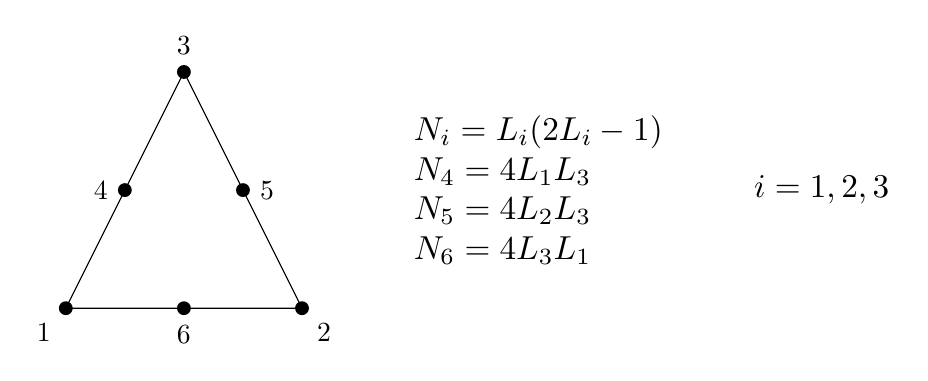
\begin{tikzpicture}[scale=3] 
 \draw (0,0) -- (1,0) -- (0.5,1) -- cycle;
 \node[circle, fill=black, inner sep=0pt, minimum size=5pt,label=below left:{1}] at (0,0) {};
 \node[circle, fill=black, inner sep=0pt, minimum size=5pt,label=below right:{2}] at (1,0) {};
 \node[circle, fill=black, inner sep=0pt, minimum size=5pt,label=above:{3}] at (0.5,1) {};
 \node[circle, fill=black, inner sep=0pt, minimum size=5pt,label=left:{4}] at (0.25,0.5) {};
 \node[circle, fill=black, inner sep=0pt, minimum size=5pt,label=right:{5}] at (0.75,0.5) {};
 \node[circle, fill=black, inner sep=0pt, minimum size=5pt,label=below:{6}] at (0.5,0.0) {};

 \node[draw=none, align=left, scale=1.2] at (2,0.5) {$N_i = L_i(2L_i - 1)$\\
                                                    $N_4 = 4L_1L_3$\\
                                                    $N_5 = 4L_2L_3$\\
                                                    $N_6 = 4L_3L_1$};

 \node[draw=none, scale=1.2] at (3.2,0.5) {$i = 1,2,3$};
\end{tikzpicture}
\end{center}
\caption{Quad Triangular Element}
\label{elemento triangular quadrático}
\end{figure}

\medskip
\noindent
\textbf{Mini Triangular Element:} 
This element is used when we have restrictions that 
prevent the use of the linear element or when we are interested in 
a better accuracy of the result as well as quad element. 
Their elementary matrices are also calculated using 
the Gaussian Quadrature. Although it is an incomplete cubic element, 
the interpolation polynomial is still of third order. 
In this way, its interpolation functions have a bubble in the center 
of the element. This element is represented by
\ref{elemento triangular mini}:

\begin{figure}[H]
\begin{center}
\begin{tikzpicture}[scale=3] 
 \draw (0,0) -- (1,0) -- (0.5,1) -- cycle;
 \node[circle, fill=black, inner sep=0pt, minimum size=5pt,label=below left:{1}] at (0,0) {};
 \node[circle, fill=black, inner sep=0pt, minimum size=5pt,label=below right:{2}] at (1,0) {};
 \node[circle, fill=black, inner sep=0pt, minimum size=5pt,label=above:{3}] at (0.5,1) {};
 \node[circle, fill=black, inner sep=0pt, minimum size=5pt,label=above:{4}] at (1/2,1/3) {};
 
 \node[draw=none, align=left, scale=1.2] at (2,0.5) {$N_i = L_1 - 9L_1L_2L_3$\\
                                                    $N_4 = 27L_1L_2L_3$};

 \node[draw=none, scale=1.2] at (3.2,0.5) {$i = 1,2,3$};
\end{tikzpicture}
\end{center}
\caption{Mini Triangular Element}
\label{elemento triangular mini}
\end{figure}





%\begin{figure}[H]
%  \centering
%  \includegraphics[scale=0.25]{./02_chaps/cap_mef/figure/mini.png}
% \caption{Funções de Interpolação para o elemento MINI.}
% \label{mini}
%\end{figure}

\medskip
Triangular elements are the most common in 2D-FE Method because 
it allows a good discretization of irregular surfaces 
due to its geometric simplicity. In this work, we use a triangular 
element with the interpolator polynomial of order one, that is, linear.
Therefore, 
the Eqs (\ref{vorticity pre matrix} to \ref{concentration pre matrix})
can be represented in matrix form by:

\begin{equation}
\begin{aligned}
 M \overset{.}{w} + u \cdot G_x w  + v \cdot G_y w & + \frac{1}{\textit{Re}} \Big[ K_{xx} + K_{yy} \Big] w
 \\[5pt]
 & + \frac{\Delta t}{2} u \Big[ u K_{xx} + v K_{yx} \Big] w 
 + \frac{\Delta t}{2} v \Big[ u K_{xy} + v K_{yy} \Big] w 
 = 0 \label{vorticity matrix}
\end{aligned}
\end{equation}

\begin{equation}
 - \Big[ K_{xx} + K_{yy} \Big] \psi + Mw = 0
\end{equation}

\begin{equation}
 Mu - G_y \psi = 0
\end{equation}

\begin{equation}
 Mv + G_x \psi = 0
\end{equation}

\begin{equation}
\begin{aligned}
 M \overset{.}{c} + u \cdot G_x c + v \cdot G_y c & + \frac{1}{\textit{ReSc}} \Big[ K_{xx} + K_{yy} \Big] c
 \\[5pt]
 & + \frac{\Delta t}{2} u \Big[ u K_{xx} + v K_{xy} \Big] c
 + \frac{\Delta t}{2} v \Big[ u K_{yx} + v K_{yy} \Big] c 
 = 0 \label{concentration matrix}
\end{aligned} 
\end{equation}

\medskip
\noindent
where the \textbf{M}, \textbf{G\textsubscript{x}}, 
\textbf{G\textsubscript{y}}, \textbf{K\textsubscript{xx}},
\textbf{K\textsubscript{xy}},
\textbf{K\textsubscript{yx}}, 
\textbf{K\textsubscript{yy}} matrices
have \textbf{np} x \textbf{np} size
(where \textit{np} is node number) and
they are defined as:

\begin{align}
  \textbf{M} & = \textbf{A} m^{e}\\
  \textbf{G\textsubscript{x}} & = \textbf{A} g_{x}^{e}\\
  \textbf{G\textsubscript{y}} & = \textbf{A} g_{y}^{e} \\
  \textbf{K\textsubscript{xx}} & = \textbf{A} k_{xx}^{e} \\
  \textbf{K\textsubscript{xy}} & = \textbf{A} k_{xy}^{e} \\
  \textbf{K\textsubscript{yx}} & = \textbf{A} k_{yx}^{e} \\
  \textbf{K\textsubscript{yy}} & = \textbf{A} k_{yy}^{e}
\end{align}

\noindent
where \textbf{A} is an assembly operator
that it assembles the elementary matrix in
global matrix, satisfying the local and global matrix index
correspondence and the
$m^{e}$, 
$g^{e}_{x}$,
$g^{e}_{y}$,
$k^{e}_{xx}$,
$k^{e}_{xy}$,
$k^{e}_{yx}$,
$k^{e}_{yy}$
are elementary matrices whose
size for the  
\textit{linear triangular element} is \textit{3}x\textit{3} and
they are defined by:


\begin{equation}
 \begin{aligned}
  m^{e} & = \int_{\Omega^{e}} N_{i}^{e} N_{j}^{e} d\Omega \\
  g_{x}^{e} & = \int_{\Omega^{e}} \frac{\partial N_{i}^{e}}{\partial x} N_{j}^{e} d\Omega \\
  g_{y}^{e} & = \int_{\Omega^{e}} \frac{\partial N_{i}^{e}}{\partial y} N_{j}^{e} d\Omega \\
  k_{xx}^{e} & = \int_{\Omega^{e}} \frac{\partial N_{i}^{e}}{\partial x} \frac{\partial N_{j}^{e}}{\partial x} \\
  k_{xy}^{e} & = \int_{\Omega^{e}} \frac{\partial N_{i}^{e}}{\partial x} \frac{\partial N_{j}^{e}}{\partial y} \\
  k_{yx}^{e} & = \int_{\Omega^{e}} \frac{\partial N_{i}^{e}}{\partial y} \frac{\partial N_{j}^{e}}{\partial x} \\
  k_{yy}^{e} & = \int_{\Omega^{e}} \frac{\partial N_{i}^{e}}{\partial y} \frac{\partial N_{j}^{e}}{\partial y}
 \end{aligned}
\end{equation}

\medskip
Thus, the governing equations in matrix form according to 
the Finite Element Method that we used in this work were:

\begin{equation} \label{final equation}
\begin{aligned}
 \frac{M}{\Delta t} w^{n+1} = \frac{M}{\Delta t} w^{n} - u \cdot G_x w^{n} & - v \cdot G_y w^{n} 
 - \frac{1}{\textit{Re}} \Big[ K_{xx} + K_{yy} \Big] w^{n}  
 \\[5pt]
 & - \frac{\Delta t}{2} u \Big[ u K_{xx} + v K_{yx} \Big] w^{n} 
 - \frac{\Delta t}{2} v \Big[ u K_{xy} + v K_{yy} \Big] w^{n} 
\end{aligned}
\end{equation}


\begin{equation}
 \Big[ K_{xx} + K_{yy} \Big] \psi = Mw
\end{equation}

\begin{equation}
 Mu = G_y \psi
\end{equation}

\begin{equation}
 Mv = - G_x \psi
\end{equation}

\begin{equation}
\begin{aligned}
 \frac{M}{\Delta t} c^{n+1} = \frac{M}{\Delta t} c^{n}  - u \cdot G_x c^{n} - v & \cdot G_y c^{n} 
 - \frac{1}{\textit{ReSc}} \Big[ K_{xx} + K_{yy} \Big] c^{n}  
 \\[5pt]
 & - \frac{\Delta t}{2} u \Big[ u K_{xx} + v K_{yx} \Big] c^{n} 
 - \frac{\Delta t}{2} v \Big[ u K_{xy} + v K_{yy} \Big] c^{n} 
\end{aligned}
\end{equation}





\chapter{\textbf{CÓDIGO NUMÉRICO}}
\label{codigo numerico}

\section{\textbf{Introdução}} 
In this chapter, we will present the main characteristics 
of the computational code developed in Python 2.7 \cite{python} 
using the object-oriented paradigm (OOP) in order to reuse the code 
in other simulations in the future. All developed classes are imported 
into the simulator (\textit{TriSim}), where the result of the 
numerical simulation is exported as presented in the 
simplified \textit{Class Diagram} (UML) of \ref{uml}. 
Initially, the \textit{script} that performs the import 
of the computational mesh for the simulation is presented. 
Then, the assembly of the global matrices is done 
respecting the correspondence between the global and local index. 
Later on, we present the application of boundary conditions for 
both \textit{Dirichlet} and \textit{Neumann}. 
Finally, the solve algorithm for the vorticity-streamfunction 
formulation with the species transport equation is presented.

\vspace{0.5cm}
\begin{figure}[H]
\begin{center}
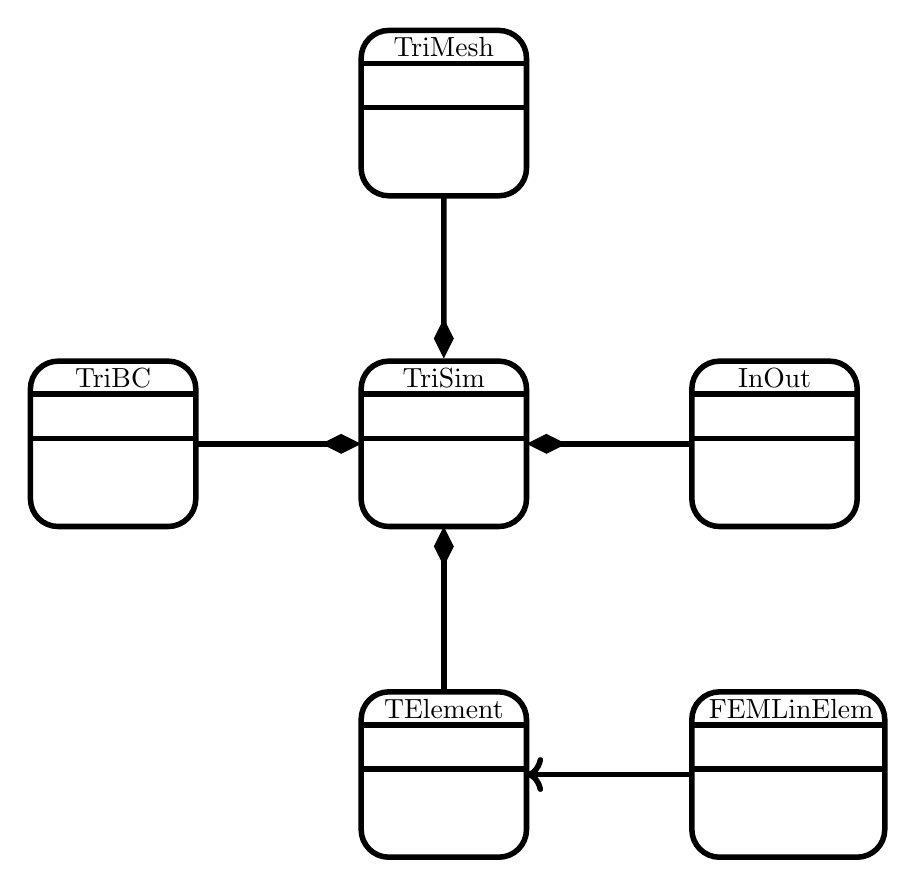
\begin{tikzpicture}[scale=0.7pt]
 \draw [rounded corners=10,line width=2pt] (0,0) rectangle ++(3,3);
 \draw [line width=2pt] (0,2.4) -- (3,2.4);
 \draw [line width=2pt] (0,1.6) -- (3,1.6);
 \node (TriSim) at (1.5,2.7) {TriSim};

 \draw [rounded corners=10,line width=2pt] (0,6) rectangle ++(3,3);
 \draw [line width=2pt] (0,8.4) -- (3,8.4);
 \draw [line width=2pt] (0,7.6) -- (3,7.6);
 \node (TriMesh) at (1.5,8.7) {TriMesh};

 \draw [rounded corners=10,line width=2pt] (6,0) rectangle ++(3,3);
 \draw [line width=2pt] (6,2.4) -- (9,2.4);
 \draw [line width=2pt] (6,1.6) -- (9,1.6);
 \node (InOut) at (7.5,2.7) {InOut};

 \draw [rounded corners=10,line width=2pt] (-6,0) rectangle ++(3,3);
 \draw [line width=2pt] (-6,2.4) -- (-3,2.4);
 \draw [line width=2pt] (-6,1.6) -- (-3,1.6);
 \node (triBC) at (-4.5,2.7) {TriBC};

 \draw [rounded corners=10,line width=2pt] (0,-6) rectangle ++(3,3);
 \draw [line width=2pt] (0,-3.6) -- (3,-3.6);
 \draw [line width=2pt] (0,-4.4) -- (3,-4.4);
 \node (TElement) at (1.5,-3.3) {TElement};

 \draw [rounded corners=10,line width=2pt] (6,-6) rectangle ++(3.5,3);
 \draw [line width=2pt] (6,-3.6) -- (9.5,-3.6);
 \draw [line width=2pt] (6,-4.4) -- (9.5,-4.4);
 \node (FEMLinElement) at (7.8,-3.3) {FEMLinElem};

 \draw [{Diamond}-,line width=2pt] (TriSim) -- (1.5,6);
 \draw [{Diamond}-,line width=2pt] (0,1.5) -- (-3,1.5);
 \draw [{Diamond}-,line width=2pt] (1.5,0) -- (1.5,-3);
 \draw [{Diamond}-,line width=2pt] (3,1.5) -- (6,1.5);
 \draw [<-,line width=2pt] (3,-4.5) -- (6,-4.5);

\end{tikzpicture}
\end{center}
\caption{Simplified Class Diagram}
\label{uml}
\end{figure}


\section{\textbf{Importação da Malha}} 
\label{trimesh}

The domain consists of an unstructured mesh generated by 
the \textit{GMSH} open-source software proposed by 
Geuzaine and Remacle (2009) \cite{gmsh} and 
it was imported into the numerical simulation by 
the \textit{TriMesh} class. 
Initially, we used a well-known computational community script to 
convert the \textit{.msh} file to a 
\textit{Python} list:

\begin{verbatim}
__________________________________________________________________________
mesh = []                             | Python list inicialization
with open("file.msh") as mesh:        | Open file 
 for line in mesh:                    | Loop file each line
  row = line.split()                  | Split file line
  mesh.append(row[:])                 | Add file line from python list 
__________________________________________________________________________
\end{verbatim}

\noindent
Then, this class returns important information for the simulation 
such as:
\textit{Nodes number} (\textbf{np}), 
\textit{Elements number} (\textbf{ne}), 
\textit{The coordinate vectors} (\textbf{x} and \textbf{y}), 
\textit{The connectivity matrix} (\textbf{IEN}) and 
\textit{The Boundary nodes}. 
The \ref{tempo malha} shows the average processing time for 
several unstructured linear triangular meshes import.

\vspace{0.5cm}
\begin{table}[H]
\centering
\begin{tabular}{ccc}
\toprule
\textbf{Nodes} & \textbf{Elements} & \textbf{AVG Processing Time} (s) \\
\midrule
10482 & 20142 & 0,6 \\
40819 & 80005 & 2,6 \\
249677 & 495289 & 16,6 \\
993091 & 2010501 & 70,4 \\
\bottomrule
\end{tabular}
\caption{Average processing time for several unstructured linear triangular mesh import}
\label{tempo malha}
\end{table}

\newpage


\section{\textbf{Montagem das Matrizes Globais}} 
\label{trielem}

Após a importação do arquivo \textit{.msh}
foi realizado a montagem das matrizes globais.
As mesmas foram inicializadas como matrizes
esparsas pela biblioteca \textit{Scipy} \cite{scipy}
e o seguinte \textit{script} foi usado para a montagem:


%\begin{algorithm}[H]
%\caption{Assembly Global Matrix}
%\begin{algorithmic}
% \For {e in range(0,ne)}
%   \State Linear\_Element\\
%   \For {i in range(0,3)}
%    \State ii = IEN[e][i]\\
%    \For {j in range(0,3)}
%     \State jj = IEN[e][j]\\
%     \State Kxx[ii][jj] += kxx\_element[i][j]
%     \State Kxy[ii][jj] += kxy\_element[i][j]
%    \State Kyx[ii][jj] += kyx\_element[i][j]
%    \State Kyy[ii][jj] += kyy\_element[i][j]
%    \State Gx[ii][jj] += gx\_element[i][j]
%    \State Gy[ii][jj] += gy\_element[i][j]
%    \State M[ii][jj] += mass\_element[i][j]\\
%   \EndFor 
%  \EndFor 
% \EndFor 
%\end{algorithmic}
%\end{algorithm}


\begin{verbatim}
__________________________________________________________________________
for e in range(0, ne):                 | loop sobre os elementos 
 linear_element(e)                     | montagem das matrizes elementares
                                         utilizando a quadratura gaussiana
 for i in range(0,3):                  
  ii = IEN[e][i]                       
  
  for j in range(0,3):                  
   jj = IEN[e][j]
                                       
   Kxx[ii,jj] += kxx_element[i][j]     |
   Kxy[ii,jj] += kxy_element[i][j]     |
   Kyx[ii,jj] += kyx_element[i][j]     |
   Kyy[ii,jj] += kyy_element[i][j]     | montagem das matrizes globais
                                       | correspondendo os índices globais
   Gx[ii,jj] += gx_element[i][j]       | e locais
   Gy[ii,jj] += gy_element[i][j]       | 
                                       |
   M[ii,jj] += mass_element[i][j]      |
__________________________________________________________________________
\end{verbatim}


\medskip
A montagem das matrizes elementares é feita pelo módulo 
\textit{linear\_element} cujo paramêtro requerido é o 
número do elemento. Esse módulo faz parte da classe \textit{TElement}
onde utiliza a quadratura gaussiana para o cálculo dos
valores das matrizes elementares. Para o elemento triangular
linear, é possível a utilização das matrizes elementares
analíticas. Para mais detalhe consultar o trabalho de Lewis,
Nithiarasu e Seetharamu (2004) \cite{lewis2004}.

\newpage
Em seguida, a matriz do lado esquerdo conhecida como 
\textit{left hand side (LHS)} é criada para as
equações da função de corrente,
velocidade e concentração respectivamente:

\begin{verbatim}
__________________________________________________________________________
LHS_psi = sps.lil_matrix.copy(K)
LHS_vx = sps.lil_matrix.copy(M)
LHS_vy = sps.lil_matrix.copy(M)
LHS_c = sps.lil_matrix.copy(M)/dt
__________________________________________________________________________
\end{verbatim}

A matriz \textit{LHS} para a equação da vorticidade
é criada durante o loop do algoritmo de solução
a fim de garantir que a mesma será sempre inicializada
utilizando as matrizes globais originais.
É necessário usarmos a função \textit{copy}
porque queremos copiar os valores das matrizes globais
e não referencia-los,
para mais detalhe consultar o \textit{Scipy Community} \cite{numpycopy}.
A \ref{tempo matrizes globais} apresenta o tempo de processamento para 
para a montagem das matrizes globais em diversas
malhas triangulares lineares não estruturadas.

\vspace{0.5cm}
\begin{table}[H]
\centering
\begin{tabular}{ccc}
\toprule
\textbf{N. Nós} & \textbf{N. Elementos} & \textbf{Tempo de Processamento} (s) \\
\midrule
10482 & 20142 & 72,9 \\
40819 & 80005 & 254,3 \\
249677 & 495289 & 1664,9 \\
993091 & 2010501 & 69059,9 \\

\bottomrule
\end{tabular}
\caption{Tempo de montagem das matrizes globais para diversas malhas triangulares não estruturadas}
\label{tempo matrizes globais}
\end{table}
                


\section{\textbf{Aplicação das Condições de Contorno}} 
\label{tricond}

Após a montagem das matrizes globais, as condições de contorno
são aplicadas. Conforme foi dito na seção \ref{trimesh}, durante a importação
da malha é possível identificarmos os nós que se encontram no
contorno do domínio. A condição onde os nós possuem seus valores 
pré definidos pelo problema em análise é conhecida como \textit{Condição 
de Dirichlet}. Sendo assim, esses nós não devem ser alterados conforme
a simulação acontece. Dessa maneira, o produto entre a coluna da matriz global cujo índice
é um nó com condição de contorno Dirichlet e o seu valor pré definido
como condição de contorno é subtraído ao vetor do
lado direito da equação de governo. Em seguida, zeramos as linhas e colunas
da matriz global que corresponde ao índice de condição de Dirichlet
e colocamos o valor de 1 na diagonal principal.

\medskip
Para exemplificar, consideraremos uma matriz 
com dimensões (\textit{np x np})
e o nó 2 como um nó localizado no
contorno do domínio onde a condição proposta
é de Dirichlet.
Desta forma, o seguinte algoritmo é feito conforme apresentado por Anjos (2007) \cite{anjos2007}:

\begin{enumerate}
 
 \vspace{0.5cm}
 \item \textbf{Localiza-se o nó de condição de contorno na matriz:}
\medskip
\begin{center}
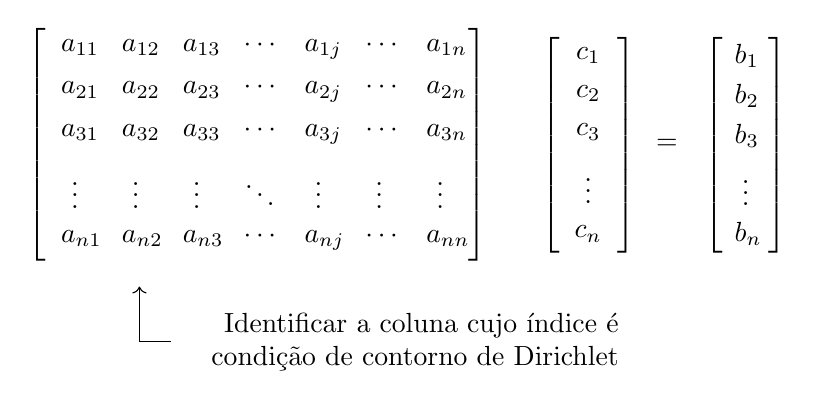
\begin{tikzpicture}
\matrix (m) [matrix of math nodes,
inner sep=0pt, column sep=0.4em,
nodes={inner sep=0.4em,text width=1.0em,align=center},
left delimiter={[},
right delimiter={]},
]
{
a_{11} & a_{12} & a_{13} & \cdots & a_{1j} & \cdots & a_{1n} \\
a_{21} & a_{22} & a_{23} & \cdots & a_{2j} & \cdots & a_{2n} \\
a_{31} & a_{32} & a_{33} & \cdots & a_{3j} & \cdots & a_{3n} \\
\vdots & \vdots & \vdots & \ddots & \vdots & \vdots & \vdots \\
a_{n1} & a_{n2} & a_{n3} & \cdots & a_{nj} & \cdots & a_{nn} \\
};
\begin{scope}[xshift=4.2cm]
\matrix (m) [matrix of math nodes,
inner sep=0pt, column sep=0.4em,
nodes={inner sep=0.4em,text width=1em,align=center},
left delimiter={[},
right delimiter={]},
]
{
c_1 \\
c_2 \\
c_3 \\
\vdots \\
c_n \\
};
\end{scope}
\begin{scope}[xshift=5.2cm]
\node {=};
\end{scope}
\begin{scope}[xshift=6.2cm]
\matrix (m) [matrix of math nodes,
inner sep=0pt, column sep=0.4em,
nodes={inner sep=0.3em,text width=0.8em,align=center},
left delimiter={[},
right delimiter={]},
]
{
b_1 \\
b_2 \\
b_3 \\
\vdots \\
b_n \\
};
\end{scope}
 \draw[<-] (-1.5,-1.8) -- (-1.5,-2.5) -- (-1.1,-2.5);
 \node [draw=none, align=right] at (2.0,-2.5) {Identificar a coluna cujo índice é \\ condição de contorno de Dirichlet};
\end{tikzpicture}
\end{center}

 \vspace{0.5cm}
 \item \textbf{Subtrai-se o produto entre a coluna onde está situado o nó da matriz e o seu valor pré definido 
com o vetor do lado direito da equação:}
\medskip
\begin{center}
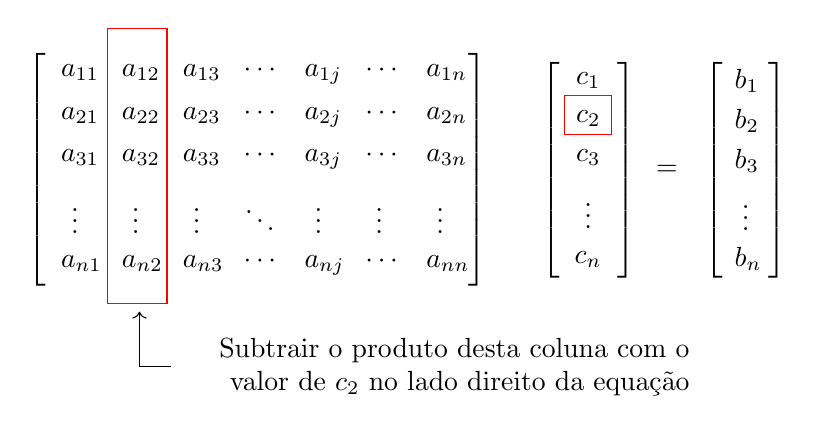
\begin{tikzpicture}
\matrix (m) [matrix of math nodes,
inner sep=0pt, column sep=0.4em,
nodes={inner sep=0.4em,text width=1.0em,align=center},
left delimiter={[},
right delimiter={]},
]
{
a_{11} & a_{12} & a_{13} & \cdots & a_{1j} & \cdots & a_{1n} \\
a_{21} & a_{22} & a_{23} & \cdots & a_{2j} & \cdots & a_{2n} \\
a_{31} & a_{32} & a_{33} & \cdots & a_{3j} & \cdots & a_{3n} \\
\vdots & \vdots & \vdots & \ddots & \vdots & \vdots & \vdots \\
a_{n1} & a_{n2} & a_{n3} & \cdots & a_{nj} & \cdots & a_{nn} \\
};
\begin{scope}[xshift=4.2cm]
\matrix (m) [matrix of math nodes,
inner sep=0pt, column sep=0.4em,
nodes={inner sep=0.4em,text width=1em,align=center},
left delimiter={[},
right delimiter={]},
]
{
c_1 \\
c_2 \\
c_3 \\
\vdots \\
c_n \\
};
\end{scope}
\begin{scope}[xshift=5.2cm]
\node {=};
\end{scope}
\begin{scope}[xshift=6.2cm]
\matrix (m) [matrix of math nodes,
inner sep=0pt, column sep=0.4em,
nodes={inner sep=0.3em,text width=0.8em,align=center},
left delimiter={[},
right delimiter={]},
]
{
b_1 \\
b_2 \\
b_3 \\
\vdots \\
b_n \\
};
\end{scope}
 %text
 \draw[<-] (-1.5,-1.8) -- (-1.5,-2.5) -- (-1.1,-2.5);
 \node [draw=none, align=right] at (2.5,-2.5) {Subtrair o produto desta coluna com o \\ valor de $c_2$ no lado direito da equação};
 %block
 \draw[red] (-1.9,1.8) -- (-1.15,1.8) -- (-1.15,-1.7) -- (-1.9,-1.7) -- cycle;
 \draw[red] (3.9,0.95) -- (4.5,0.95) -- (4.5,0.45) -- (3.9,0.45) -- cycle;
\end{tikzpicture}
\end{center}

\newpage
isto é,

\medskip
\begin{center}
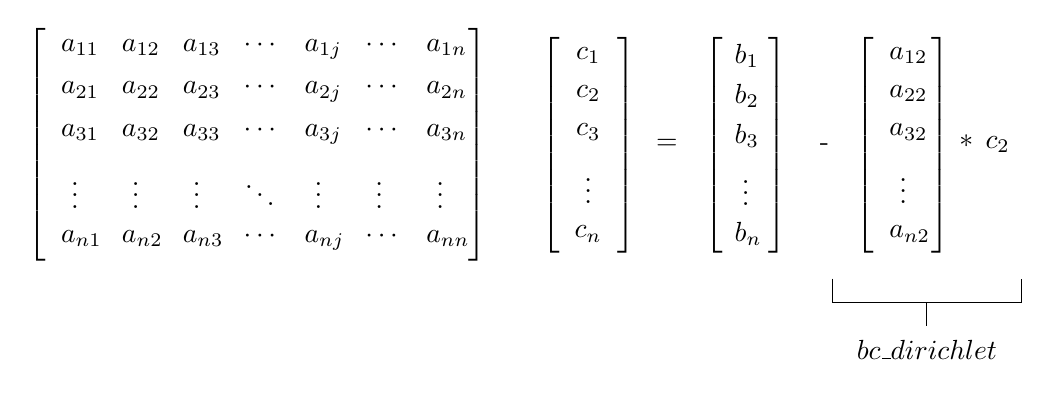
\begin{tikzpicture}
\matrix (m) [matrix of math nodes,
inner sep=0pt, column sep=0.4em,
nodes={inner sep=0.4em,text width=1.0em,align=center},
left delimiter={[},
right delimiter={]},
]
{
a_{11} & a_{12} & a_{13} & \cdots & a_{1j} & \cdots & a_{1n} \\
a_{21} & a_{22} & a_{23} & \cdots & a_{2j} & \cdots & a_{2n} \\
a_{31} & a_{32} & a_{33} & \cdots & a_{3j} & \cdots & a_{3n} \\
\vdots & \vdots & \vdots & \ddots & \vdots & \vdots & \vdots \\
a_{n1} & a_{n2} & a_{n3} & \cdots & a_{nj} & \cdots & a_{nn} \\
};
\begin{scope}[xshift=4.2cm]
\matrix (m) [matrix of math nodes,
inner sep=0pt, column sep=0.4em,
nodes={inner sep=0.4em,text width=1em,align=center},
left delimiter={[},
right delimiter={]},
]
{
c_1 \\
c_2 \\
c_3 \\
\vdots \\
c_n \\
};
\end{scope}
\begin{scope}[xshift=5.2cm]
\node {=};
\end{scope}
\begin{scope}[xshift=6.2cm]
\matrix (m) [matrix of math nodes,
inner sep=0pt, column sep=0.4em,
nodes={inner sep=0.3em,text width=0.8em,align=center},
left delimiter={[},
right delimiter={]},
]
{
b_1 \\
b_2 \\
b_3 \\
\vdots \\
b_n \\
};
\end{scope}
\begin{scope}[xshift=7.2cm]
\node {-};
\end{scope}
\begin{scope}[xshift=8.2cm]
\matrix (m) [matrix of math nodes,
inner sep=0pt, column sep=0.4em,
nodes={inner sep=0.4em,text width=1em,align=center},
left delimiter={[},
right delimiter={]},
]
{
a_{12} \\
a_{22} \\
a_{32} \\
\vdots \\
a_{n2} \\
};
\end{scope}
\begin{scope}[xshift=9.0cm]
\node {*};
\end{scope}
\begin{scope}[xshift=9.4cm]
 \node {$c_2$};
\end{scope}
 %text
 \node [draw=none, align=right] at (8.5,-2.6) {$bc\_dirichlet$};
 %block
 \draw (7.3,-1.7) -- (7.3,-2.0) -- (9.7,-2.0) -- (9.7,-1.7);
 \draw (8.5,-2.0) -- (8.5,-2.3);
\end{tikzpicture}
\end{center}

 \vspace{0.5cm}
 \item \textbf{Preenche-se com zeros a coluna e a linha da matriz correspondente ao nó de condição de contorno:}
\medskip
\begin{center}
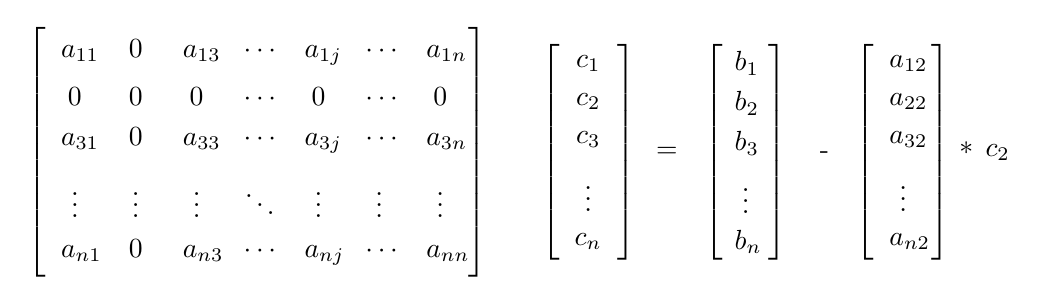
\begin{tikzpicture}
\matrix (m) [matrix of math nodes,
inner sep=0pt, column sep=0.4em,
nodes={inner sep=0.4em,text width=1.0em,align=center},
left delimiter={[},
right delimiter={]},
]
{
a_{11} & 0 & a_{13} & \cdots & a_{1j} & \cdots & a_{1n} \\
0 & 0 & 0 & \cdots & 0 & \cdots & 0 \\
a_{31} & 0 & a_{33} & \cdots & a_{3j} & \cdots & a_{3n} \\
\vdots & \vdots & \vdots & \ddots & \vdots & \vdots & \vdots \\
a_{n1} & 0 & a_{n3} & \cdots & a_{nj} & \cdots & a_{nn} \\
};
\begin{scope}[xshift=4.2cm]
\matrix (m) [matrix of math nodes,
inner sep=0pt, column sep=0.4em,
nodes={inner sep=0.4em,text width=1em,align=center},
left delimiter={[},
right delimiter={]},
]
{
c_1 \\
c_2 \\
c_3 \\
\vdots \\
c_n \\
};
\end{scope}
\begin{scope}[xshift=5.2cm]
\node {=};
\end{scope}
\begin{scope}[xshift=6.2cm]
\matrix (m) [matrix of math nodes,
inner sep=0pt, column sep=0.4em,
nodes={inner sep=0.3em,text width=0.8em,align=center},
left delimiter={[},
right delimiter={]},
]
{
b_1 \\
b_2 \\
b_3 \\
\vdots \\
b_n \\
};
\end{scope}
\begin{scope}[xshift=7.2cm]
\node {-};
\end{scope}
\begin{scope}[xshift=8.2cm]
\matrix (m) [matrix of math nodes,
inner sep=0pt, column sep=0.4em,
nodes={inner sep=0.4em,text width=1em,align=center},
left delimiter={[},
right delimiter={]},
]
{
a_{12} \\
a_{22} \\
a_{32} \\
\vdots \\
a_{n2} \\
};
\end{scope}
\begin{scope}[xshift=9.0cm]
\node {*};
\end{scope}
\begin{scope}[xshift=9.4cm]
 \node {$c_2$};
\end{scope}
\end{tikzpicture}
\end{center}


 \vspace{0.5cm}
 \item \textbf{Coloca-se 1 na diagonal principal da matriz cujo índice é o nó de condição de contorno:}
\medskip
\begin{center}
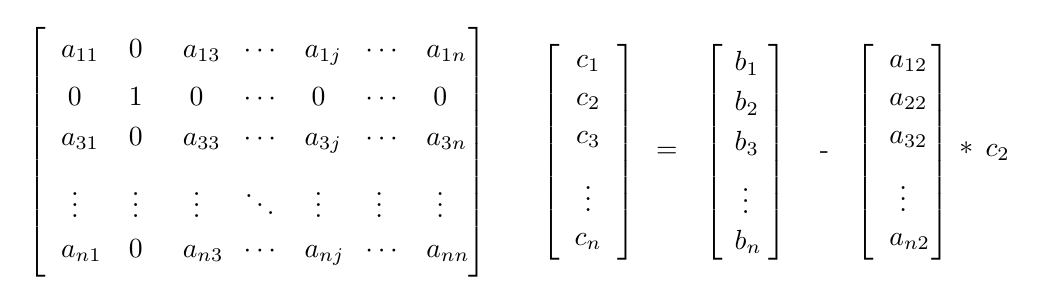
\begin{tikzpicture}
\matrix (m) [matrix of math nodes,
inner sep=0pt, column sep=0.4em,
nodes={inner sep=0.4em,text width=1.0em,align=center},
left delimiter={[},
right delimiter={]},
]
{
a_{11} & 0 & a_{13} & \cdots & a_{1j} & \cdots & a_{1n} \\
0 & 1 & 0 & \cdots & 0 & \cdots & 0 \\
a_{31} & 0 & a_{33} & \cdots & a_{3j} & \cdots & a_{3n} \\
\vdots & \vdots & \vdots & \ddots & \vdots & \vdots & \vdots \\
a_{n1} & 0 & a_{n3} & \cdots & a_{nj} & \cdots & a_{nn} \\
};
\begin{scope}[xshift=4.2cm]
\matrix (m) [matrix of math nodes,
inner sep=0pt, column sep=0.4em,
nodes={inner sep=0.4em,text width=1em,align=center},
left delimiter={[},
right delimiter={]},
]
{
c_1 \\
c_2 \\
c_3 \\
\vdots \\
c_n \\
};
\end{scope}
\begin{scope}[xshift=5.2cm]
\node {=};
\end{scope}
\begin{scope}[xshift=6.2cm]
\matrix (m) [matrix of math nodes,
inner sep=0pt, column sep=0.4em,
nodes={inner sep=0.3em,text width=0.8em,align=center},
left delimiter={[},
right delimiter={]},
]
{
b_1 \\
b_2 \\
b_3 \\
\vdots \\
b_n \\
};
\end{scope}
\begin{scope}[xshift=7.2cm]
\node {-};
\end{scope}
\begin{scope}[xshift=8.2cm]
\matrix (m) [matrix of math nodes,
inner sep=0pt, column sep=0.4em,
nodes={inner sep=0.4em,text width=1em,align=center},
left delimiter={[},
right delimiter={]},
]
{
a_{12} \\
a_{22} \\
a_{32} \\
\vdots \\
a_{n2} \\
};
\end{scope}
\begin{scope}[xshift=9.0cm]
\node {*};
\end{scope}
\begin{scope}[xshift=9.4cm]
 \node {$c_2$};
\end{scope}
\end{tikzpicture}
\end{center}

 \vspace{0.5cm}
 \item \textbf{Localiza-se o próximo nó e executa-se o passo novamente.}
\end{enumerate}

\newpage
\noindent
A implementação deste algoritmo foi realizado pelo seguinte \textit{script}:
\begin{verbatim}
__________________________________________________________________________
 for mm in ibc:                        | loop sobre os nós do contorno
  bc_dirichlet -= LHS[:,mm]*bc_1[mm]   | passo 2
  LHS[:,mm] = 0.0                      | passo 3 - zerar colunas
  LHS[mm,:] = 0.0                      | passo 3 - zerar linhas
  LHS[mm,mm] = 1.0                     | passo 4 - 1 na diagonal principal
  bc_dirichlet[mm] = bc_1[mm]          | imputando o valor da condição
                                       | de Dirichlet no índice
                                       | correspondente
__________________________________________________________________________
\end{verbatim}

\noindent
onde \textit{ibc} é uma lista que contém todos os nós do contorno
cuja condição é de Dirichlet e
\textit{$bc\_1$} é um vetor auxiliar com dimensão \textit{np}
onde o valor da condição de Dirichlet é imputada em cada índice correspondente.
O símbolo -= garante que a contribuição de cada nó cuja
condição seja de Dirichlet seja computada.
Este procedimento deverá ser realizado para cada um das \textit{LHS}.
A \ref{tempo contorno} apresenta o tempo de processamento para 
a aplicação das condições de contorno de \textit{Dirichlet} em diversas
malhas triangulares lineares não estruturadas.

\vspace{0.5cm}
\begin{table}[H]
\centering
\begin{tabular}{ccc}
\toprule
\textbf{N. Nós} & \textbf{N. Elementos} & \textbf{Tempo de Processamento} (s) \\
\midrule
10482 & 20142 & 6,8 \\
40819 & 80005 & 37,5 \\
249677 & 495289 & 467,7 \\
993091 & 2010501 & 3720,6 \\
\bottomrule
\end{tabular}
\caption{Tempo processamento para as condições de contorno para diversas malhas triangulares não estruturadas}
\label{tempo contorno}
\end{table}
 

\medskip
Outro tipo de condição de contorno muito comum é aquela onde existe um
fluxo nos contornos do domínio. Essa condição de contorno é conhecida
como \textit{Condição de Neumann} e na formulação variacional é chamada
de \textit{Condição Natural}. Diferente da condição de Dirichlet,
esse tipo de condição de contorno não afeta a matriz global do lado esquerdo quando
o fluxo é constante. Devemos apenas somar a sua contribuição
no vetor do lado direito da equação, isto é:

\begin{center}
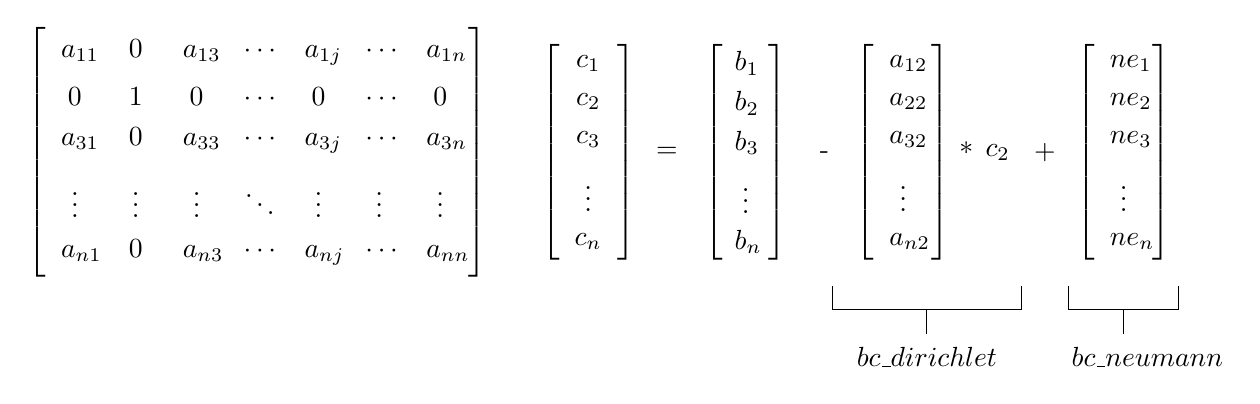
\begin{tikzpicture}
\matrix (m) [matrix of math nodes,
inner sep=0pt, column sep=0.4em,
nodes={inner sep=0.4em,text width=1.0em,align=center},
left delimiter={[},
right delimiter={]},
]
{
a_{11} & 0 & a_{13} & \cdots & a_{1j} & \cdots & a_{1n} \\
0 & 1 & 0 & \cdots & 0 & \cdots & 0 \\
a_{31} & 0 & a_{33} & \cdots & a_{3j} & \cdots & a_{3n} \\
\vdots & \vdots & \vdots & \ddots & \vdots & \vdots & \vdots \\
a_{n1} & 0 & a_{n3} & \cdots & a_{nj} & \cdots & a_{nn} \\
};
\begin{scope}[xshift=4.2cm]
\matrix (m) [matrix of math nodes,
inner sep=0pt, column sep=0.4em,
nodes={inner sep=0.4em,text width=1em,align=center},
left delimiter={[},
right delimiter={]},
]
{
c_1 \\
c_2 \\
c_3 \\
\vdots \\
c_n \\
};
\end{scope}
\begin{scope}[xshift=5.2cm]
\node {=};
\end{scope}
\begin{scope}[xshift=6.2cm]
\matrix (m) [matrix of math nodes,
inner sep=0pt, column sep=0.4em,
nodes={inner sep=0.3em,text width=0.8em,align=center},
left delimiter={[},
right delimiter={]},
]
{
b_1 \\
b_2 \\
b_3 \\
\vdots \\
b_n \\
};
\end{scope}
\begin{scope}[xshift=7.2cm]
\node {-};
\end{scope}
\begin{scope}[xshift=8.2cm]
\matrix (m) [matrix of math nodes,
inner sep=0pt, column sep=0.4em,
nodes={inner sep=0.4em,text width=1em,align=center},
left delimiter={[},
right delimiter={]},
]
{
a_{12} \\
a_{22} \\
a_{32} \\
\vdots \\
a_{n2} \\
};
\end{scope}
\begin{scope}[xshift=9.0cm]
\node {*};
\end{scope}
\begin{scope}[xshift=9.4cm]
 \node {$c_2$};
\end{scope}
\begin{scope}[xshift=10.0cm]
\node {+};
\end{scope}
\begin{scope}[xshift=11.0cm]
\matrix (m) [matrix of math nodes,
inner sep=0pt, column sep=0.4em,
nodes={inner sep=0.4em,text width=1em,align=center},
left delimiter={[},
right delimiter={]},
]
{
ne_{1} \\
ne_{2} \\
ne_{3} \\
\vdots \\
ne_{n} \\
};
\end{scope}
 %text
 \node [draw=none, align=right] at (8.5,-2.6) {$bc\_dirichlet$};
 \node [draw=none, align=right] at (11.3,-2.6) {$bc\_neumann$};
 %block
 \draw (7.3,-1.7) -- (7.3,-2.0) -- (9.7,-2.0) -- (9.7,-1.7);
 \draw (8.5,-2.0) -- (8.5,-2.3);
 \draw (10.3,-1.7) -- (10.3,-2.0) -- (11.7,-2.0) -- (11.7,-1.7);
 \draw (11.0,-2.0) -- (11.0,-2.3);
\end{tikzpicture}
\end{center}

\medskip
Como foi mencionado no capítulo \ref{metodo dos elementos finitos}, possuímos apenas condição de Dirichlet neste trabalho.
A seguir, porém, apresentaremos a implementação desse tipo de condição.
A fim de exemplificar, consideraremos o termo de contorno da equação
\ref{diffusion2_concentration}, isto é:

\begin{equation} 
 \frac{1}{\textit{ReSc}} \int_{\Gamma} \eta \nabla c \cdot \textbf{n} d\Gamma
\end{equation}

\medskip
\noindent
onde $\nabla c$ é o fluxo que será considerado constante. 
Após a discretização pela formulação de Galerkin, 
possuímos a seguinte expressão:

\begin{equation} 
 \frac{1}{\textit{ReSc}} \int_{\Gamma} N_j \nabla c \cdot \textbf{n} d\Gamma
\end{equation}

\medskip
\noindent
isto é:

\begin{equation} 
 \frac{1}{\textit{ReSc}} \Bigg[ \frac{length  \nabla c}{2} \Bigg]
\end{equation}

\medskip
\noindent
onde a variável \textit{$length$} é o comprimento da aresta do elemento. 
Considerando um domínio bidimensional onde 
\textit{$i$} é um nó no contorno deste domínio e
\textit{$i-1$} e \textit{$i+1$} são seus vizinhos neste contorno,
as arestas do nó \textit{$i$} podem ser
representadas por:

\begin{figure}[h!]
\begin{center}
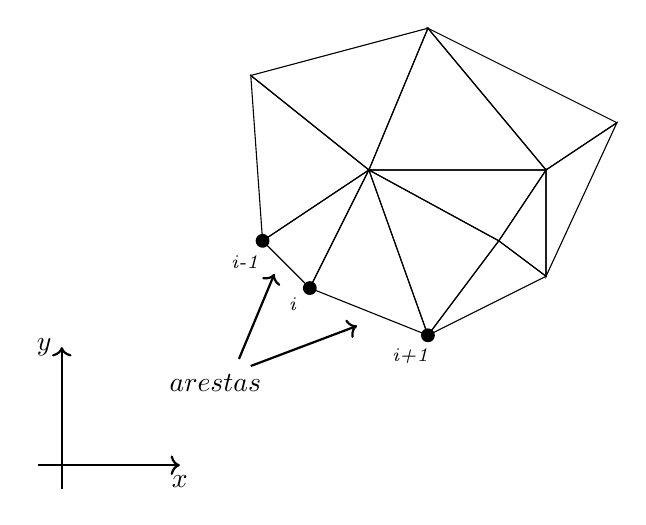
\begin{tikzpicture}[scale=3]
 \draw (0.75,0.75) -- (1.25,0.55) -- (1.00,1.25) -- cycle;
 \draw (0.75,0.75) -- (0.55,0.95) -- (1.00,1.25) -- cycle;
 \draw (1.25,0.55) -- (1.55,0.95) -- (1.00,1.25) -- cycle;
 \draw (1.55,0.95) -- (1.75,1.25) -- (1.00,1.25) -- cycle;
 \draw (1.75,1.25) -- (2.05,1.45) -- (1.25,1.85) -- cycle;
 \draw (1.25,1.85) -- (1.00,1.25) -- (1.75,1.25) -- cycle;
 \draw (1.25,0.55) -- (1.55,0.95) -- (1.75,0.80) -- cycle;
 \draw (1.55,0.95) -- (1.75,0.80) -- (1.75,1.25) -- cycle;
 \draw (1.75,0.80) -- (1.75,1.25) -- (2.05,1.45) -- cycle;
 \draw (0.55,0.95) -- (1.00,1.25) -- (0.50,1.65) -- cycle;
 \draw (1.00,1.25) -- (0.50,1.65) -- (1.25,1.85) -- cycle;
 \node[circle,fill=black, inner sep=0pt, minimum size=5pt] at (0.75,0.75) {};
 \node[circle,fill=black, inner sep=0pt, minimum size=5pt] at (0.55,0.95) {};
 \node[circle,fill=black, inner sep=0pt, minimum size=5pt] at (1.25,0.55) {};
 \node at (0.68,0.68) {\scriptsize \textit{i}};
 \node at (0.48,0.86) {\scriptsize \textit{i-1}};
 \node at (1.18,0.46) {\scriptsize \textit{i+1}};
 \draw [->,thick] (0.45,0.45)--(0.60,0.81);
 \draw [->,thick] (0.50,0.42)--(0.95,0.59);
 \draw [->,thick] (-0.3,-0.1)--(-0.3,0.5) node[left] {$y$};
 \draw [->,thick] (-0.4,0)--(0.2,0) node[below] {$x$};
 \node [draw=none] at (0.35,0.35) {$arestas$};
\end{tikzpicture}
\end{center}
\caption{Arestas vizinhas de um nó}
\end{figure}

\newpage
\noindent
onde a aresta à esquerda do nó \textit{$i$} é constituída
pelos nós \textit{$i-1$} e \textit{$i$}, enquanto a 
aresta à direita é constituída pelos nós \textit{$i$} e \textit{$i+1$}. 
Desta maneira podemos observar que o nó \textit{$i$} recebe
contribuição das aresta a sua esquerda e a sua direita. 
O \textit{script} a seguir é usado para a implementação
da condição de contorno de Neumann quando requerida:


\begin{verbatim}
__________________________________________________________________________
 for i in range(0, len(neumann_edges)):   | loop sobre as arestas neumann
 
  p1 = neumann_edges[i][1]                | os nós que constituem
  p2 = neumann_edges[i][2]                | uma aresta

  x = x[p1] - x[p2]                       | calculo do comprimento
  y = y[p1] - y[p2]                       | de uma aresta
  length = numpy.sqrt(x**2 + y**2)        | 

  bc_neumann[p1] += (length*nabla_c) / 2. | imputando o valor da condição
  bc_neumann[p2] += (length*nabla_c) / 2. | de Neumann no índice
                                          | correspondente.
__________________________________________________________________________

\end{verbatim}

\noindent
onde \textit{neumann\_edges} é uma lista que contém os nós presentes em
uma aresta cuja condição é de Neumann, \textit{p1} e \textit{p2} são os nós 
presentes na aresta, \textit{x} e \textit{y} são as coordenadas de cada nó,
\textit{length} é o comprimento da aresta, \textit{nabla\_c} é o fluxo
adimensional modelado no problema físico e \textit{numpy} é uma biblioteca
numérica do \textit{Python} no qual estamos usando a função da raiz
quadrada (\textit{numpy.sqrt}).
O símbolo += garante que a contribuição das aresta à esquerda e
à direita seja computada.
               


\section{\textbf{Algoritmo de Solução}} 
\label{simulador}

The main difficulty in implementation of 
vorticity-streamfunction formulation 
is the boundary conditions of the vorticity. 
Briefly, the solve algorithm used was:

\vspace{0.5cm}
% Define block styles
\tikzstyle{block} = [rectangle, draw, fill=gray!10!,
    text width=25em, text centered, draw,scale=0.7,text=black!90!]
\tikzstyle{line} = [draw, -latex',scale=0.75]



\begin{figure}[h!]
\begin{center}
\begin{tikzpicture}[node distance = 1.0cm,auto]
    % Place nodes
    \node [block] (step1) {Import mesh};
    \node [block, below of=step1] (step2) {Calculate Gaussian Quadradure and Assemble Matrix};
    \node [block, below of=step2] (step3) {Inicialize Vorticity and Streamfunction};
    \node [block, below of=step3] (step4) {Calculate Laplacian smoothing and ALE velocity};
    \node [block, below of=step4] (step5) {Move Nodes};
    \node [block, below of=step5] (step6) {Calculate Gaussian Quadradure and Assemble Matrix};
    \node [block, below of=step6] (step7) {Calculate vorticity boundary condition};
    \node [block, below of=step7] (step8) {Calculate semi-Lagrangian and Vorticity field};
    \node [block, below of=step8] (step9) {Calculate streamfunction field};
    \node [block, below of=step9] (step10) {Calculate velocity field};
    \node [block, below of=step10] (step11) {Calculate concentration field};
    \node [right of=step4, node distance=4cm] (initialLoop) {};
    \node [right of=step11, node distance=4cm] (finalLoop) {};
    \node [right of=step7, node distance=5.5cm] (textLoop) {};

    \node [draw=none, align=center,scale=0.7,text=black!80!] at (textLoop) {Repeat the procedure \\ for the next time step \\ until the steady state};
    % Draw edges
    \path [line] (step1) -- (step2);
    \path [line] (step2) -- (step3);
    \path [line] (step3) -- (step4);
    \path [line] (step4) -- (step5);
    \path [line] (step5) -- (step6);
    \path [line] (step6) -- (step7);
    \path [line] (step7) -- (step8);
    \path [line] (step8) -- (step9);
    \path [line] (step9) -- (step10);
    \path [line] (step10) -- (step11);
    \path [line,dashed] (step11) -- (finalLoop) -- (initialLoop) |- (step4);
\end{tikzpicture}
\end{center}
\caption{Solve algorithm for Vorticity-Streamfunction Formulation with Species Transport Equation}
\label{solution algorithm} 
\end{figure}  


\medskip
In order to facilitate its implementation in other research, 
we will describe each step of the algorithm in detail. 
The equations are in their matrix form:

\begin{enumerate}
 \item \textbf{Inicialize Vorticity field:}
 \begin{equation}
  Mw = G_{x}v - G_{y}u \notag
 \end{equation}

 \item \textbf{Inicialize Streamfuntion field:}
  \begin{equation}
  \Big[ K_{xx} + K_{yy} \Big] \psi = Mw \notag
  \end{equation}
  \textit{
It is necessary to apply the boundary conditions of $\psi $ in 
the LHS matrix, its lines and columns must be zeros and 
the contribution of the cboundary indices in the vector to the right of the equation, as explained in the section \ ref {tricond}.}


 \item \textbf{Calcular as condições de contorno da vorticidade utilizando a equação:}
 \begin{equation}
  Mw = G_{x}v - G_{y}u \notag
 \end{equation}
 \textit{Após resolvermos esta equação, possuímos os valores de $w$ para todos
 os nós do domínio, mas usaremos apenas os nós do contorno
 para zerar as linhas e as colunas da matriz da equação da vorticidade 
 e sua contribuição no lado direito. Deve-se garantir que a matriz LHS 
 seja inicializada em sua forma original em cada passo de tempo. 
 Para isso, é feito a cada passo de tempo:}

\begin{verbatim}
_____________________________________________________________________
LHS_w = sps.lil_matrix.copy(M)/dt
_____________________________________________________________________
\end{verbatim}

 \textit{O script para zerar as linhas e as colunas é
 semelhante à aplicação da condição de Dirichlet
 que foi explicado na seção \ref{tricond},
 exceto à utilização do vetor auxiliar bc\_1 que
 foi substituído pelo $w$ calculado na
 equação $Mw = G_{x}v - G_{y}u$}

\begin{verbatim}
_____________________________________________________________________
for mm in ibc:                   | loop sobre os nós do contorno de w
 bc_dirichlet = LHS[:,mm]*w[mm]  | o vetor bc_1 é substituído por w
 LHS[:,mm] = 0.0                     
 LHS[mm,:] = 0.0                     
 LHS[mm,mm] = 1.0                    
 bc_dirichlet[mm] = w[mm]        | o vetor bc_1 é substituído por w
_____________________________________________________________________
\end{verbatim}

 \item \textbf{Calcular a vorticidade pela equação:}
  \begin{equation}
  \begin{aligned}
   \frac{M}{\Delta t} w^{n+1}
   =  \frac{M}{\Delta t} w^{n}
   - u \cdot G_x w^{n}
   &- v \cdot G_y w^{n} 
   - \frac{1}{\textit{Re}} \Big[ K_{xx} + K_{yy} \Big] w^{n}
   \\
   & - u
   \frac{\Delta t}{2}
   \big[
   u K_{xx}
   + v K_{yx}
   \big]
   w^{n} 
   - v
   \frac{\Delta t}{2}
   \Big[
   u K_{xy}
   + v K_{yy}
   \Big]
   w^{n} \notag
  \end{aligned}
  \end{equation}
  \textit{onde $w^{n}$ é a vorticidade calculada no passo de tempo anterior 
  e $w^{n+1}$ é a vorticidade que será calculada no passo de tempo em análise. 
  É necessário aplicar as condições de contorno de $w$ na matriz a esquerda da equação
  zerando suas linhas e colunas e a contribuição das colunas dos índices de contorno 
  no vetor a direita da equação,
  como foi explicado no passo 3.}

 \item \textbf{Calcular a função de corrente pela equação:}
  \begin{equation}
  \Big[ K_{xx} + K_{yy} \Big] \psi = Mw \notag
  \end{equation}
  \textit{É necessário aplicar as condições de contorno de $\psi$ na matriz a esquerda da equação
  zerando suas linhas e colunas e a contribuição das colunas dos índices de contorno 
  no vetor a direita da equação,
  conforme explicado na seção \ref{tricond}.}


 \item \textbf{Calcular a velocidade pela equação:}
  \begin{align}
   & Mu = G_{y}\psi  \notag \\
   & Mv = -G_{x}\psi \notag
  \end{align}
  \textit{É necessário aplicar as condições de contorno de u e v em suas 
  respectivas matrizes a esquerda de cada equação
  zerando suas linhas e colunas e a contribuição das colunas dos índices de contorno 
  no vetor a direita de cada equação,
  conforme explicado na seção anterior.}


 \item \textbf{Calcular a concentração pela equação:}
  \begin{equation}
  \begin{aligned}
   \frac{M}{\Delta t} c^{n+1}
   =  \frac{M}{\Delta t} c^{n}
   - u \cdot G_x c^{n}
   & - v \cdot G_y c^{n} 
   - \frac{1}{\textit{ReSc}} \Big[ K_{xx} + K_{yy} \Big] c^{n}
   \\
   & - u
   \frac{\Delta t}{2}
   \big[
   u K_{xx}
   + v K_{yx}
   \big]
   c^{n} 
   - v
   \frac{\Delta t}{2}
   \Big[
   u K_{xy}
   + v K_{yy}
   \Big]
   c^{n} \notag
  \end{aligned}
  \end{equation}
  \textit{Onde $c^{n}$ é a concentração calculada no passo de tempo anterior 
  e $c^{n+1}$ é a concentração que será calculada no passo de tempo em análise. 
  É necessário aplicar as condições de contorno de c na matriz a esquerda da equação
  zerando suas linhas e colunas e a contribuição das colunas dos índices de contorno 
  no vetor a direita da equação,
  conforme explicado na seção anterior.}


 \item \textbf{Retornar ao passo 3 e repetir o procedimento para outro
 passo de tempo.}
\end{enumerate}

\newpage
\noindent
Os passos 1 e 2 ficam fora do \textit{loop} do tempo, enquanto
os passos de 3 a 7 encontram-se dentro do \textit{loop}.
O procedimento para zerar as linhas e as colunas das matrizes globais
pode ser feito antes do \textit{loop}, exceto para o caso
da vorticidade em que a cada passo de tempo devemos zerar as linhas
e as colunas das matrizes globais e atribuir a contribuição dessas colunas
no vetor a direita da equação.

\medskip
\noindent
A seguir será apresentado o \textit{script} usado na solução da equação da 
vorticidade. A mesma ideia foi realizada para cada equação de governo,
alterando apenas o vetor do lado direito e as contribuições das condições
de contorno. Foi utilizado um método iterativo de solução para sistemas
lineares conhecido como \textit{Gradientes Conjugados}.

\begin{verbatim}
_________________________________________________________________________
 RHS = sps.lil_matrix.dot(np.copy(M)/dt,w)\ 
     - np.multiply(vx,sps.lil_matrix.dot(Gx,w))\
     - np.multiply(vy,sps.lil_matrix.dot(Gy,w))\
     - (1.0/Re)*sps.lil_matrix((Kxx+Kyy),w)\
     - (dt/2.0)*np.multiply(u,(np.multiply(u,sps.lil_matrix.dot(Kxx,w))\ 
                             + np.multiply(v,sps.lil_matrix.dot(Kyx,w))))\
     - (dt/2.0)*np.multiply(v,(np.multiply(u,sps.lil_matrix.dot(Kxy,w))\ 
                             + np.multiply(v,sps.lil_matrix.dot(Kyy,w))))
 
 RHS = RHS + (1/Re)*bc_neumann
 RHS = np.multiply(RHS,bc_2)
 RHS = RHS + bc_dirichlet
 
 w = scipy.sparse.linalg.cg(LHS,RHS,w, maxiter=1.0e+05, tol=1.0e-05)
 w = w[0].reshape((len(w[0]),1))
__________________________________________________________________________
\end{verbatim}

\noindent
Onde \textit{RHS} é o vetor do lado direito da equação e significa
\textit{right hand side} e \textit{bc\_2} é um vetor auxiliar
no qual garante que somente os nós sem condição de Dirichlet sejam
resolvidos. Ele consiste em um vetor com dimensões \textit{np}
onde possui o valor de 1 nos índices cujos nós não possuem
condição de Dirichlet e o valor 0 nos índices restantes, isto é,
os nós que possuem condição de Dirichlet. Vale ressaltar que o
vetor \textit{bc\_2} é diferente para cada equação já que os
contornos cuja condição é de Dirichlet variam de equação para equação,
ou seja, o vetor \textit{bc\_2} da equação da vorticidade é
diferente da equação de concentração. O primeiro bloco do \textit{script}
acima consiste no lado direito da equação (\ref{final equation}).
O segundo bloco refere-se a contribuição das condições de Neumann
(para esta simulação é nula) e de Dirichlet, além da aplicação do vetor
auxiliar \textit{bc\_2}. O terceiro bloco consiste na solução da
equação pelo método iterativo dos \textit{Gradientes Conjugados}.





\chapter{\textbf{VALIDAÇÃO DO CÓDIGO NUMÉRICO}}
\label{validacao}

\section{\textbf{Introdução}} 

In this chapter, we will present the results obtained from 
four cases with the numerical simulation of the Navier Stokes 
equation using the vorticity-streamfunction formulation with 
the species transport equation, where we have incompressible 
and monophase two-dimensional flow for all cases
in an Arbitrary Lagrangian-Eulerian context
using the semi-Lagrangian Method. 
In all simulations, were considered the $\beta_{1}=0$ 
and $\beta_{2}=1$. 
Therefore, the computational mesh velocity is
calculated using only the Laplacian smoothing velocity.

\medskip
The first section is about \textit{Couette flow} and 
the numerical solution is compared with the analytical solution. 
The second section is about the \textit{Poiseuille flow},
where the no-slip condition is applied 
and the numerical solution is also compared with 
the analytical solution. The third section refers to the flow 
of \textit {Poiseuille} in the half domain, where the 
free slip condition is applied on the axis of symmetry. 
The fourth section refers to the (\textit{lid-driven cavity flow}) 
and the solution is compared with the results presented 
by Ghia et al. (1982) \cite{ghia1982} and 
Marchi et al. (2009) \cite{marchi2009} for several Reynold numbers. 
Lastly, the comparison of the semi-Lagrangian Method in a unstructured
linear and quadratic triangular mesh is done
for the transport of a scalar 
submitted to a pure advection flow is presented.

\medskip
All numerical simulations were performed on the computers 
of \textit {Numerical Simulations Laboratory (LEN)} 
of \textit {Environmental Simulations in Reservoirs and 
Study Group (GESAR)} with the following configuration:

\begin{itemize}
 \item AMD FX-8350 4GHz with 8 core, 32Gb RAM Memory, 1000Gb of HD.
       LINUX Ubuntu 16.04 LTS. The numerical code implementarion was
       performed using Python 2.7 language
\end{itemize}

\newpage


\section{\textbf{Escoamento de Couette}} 
\label{couette}

A monophase, steady and fully developed flow of a 
Newtonian and incompressible fluid between parallel horizontal 
plates, where the lower plate moves with \textit{$U_{bottom}$} 
velocity and the upper plate moves with \textit{$ U_{top}$}, 
is known as \textit{Couette flow}. The \ref{couette}
 presents schematically this flow and the profile of the expected velocity field.

\begin{figure}[H]
\begin{center}
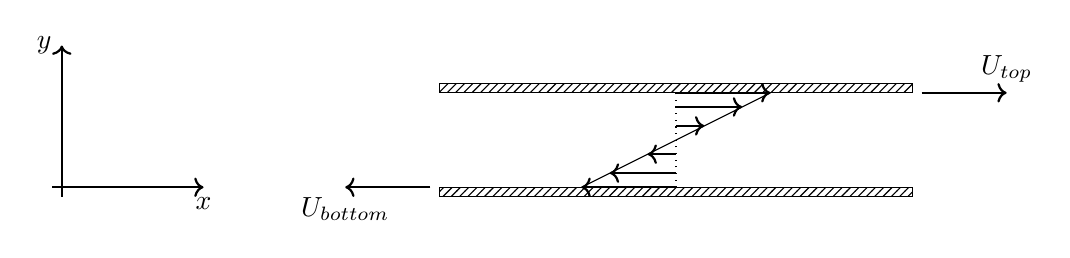
\begin{tikzpicture}[scale=1.2]
 \draw [pattern=north east lines] (0,0) -- (0,-0.1) -- (5,-0.1) -- (5,0) -- cycle;
 \draw [pattern=north east lines] (0,1) -- (0,1.1) -- (5,1.1) -- (5,1) -- cycle;

 \draw [->,thick] (5.1,1)--(6,1) node[above] {$U_{top}$};
 \draw [->,thick] (-0.1,0)--(-1,0) node[below] {$U_{bottom}$};
 
 \draw [->,thick] (-4,-0.1)--(-4,1.5) node[left] {$y$};
 \draw [->,thick] (-4.1,0)--(-2.5,0) node[below] {$x$};
 
 \draw [dotted] (2.5,0.0) to (2.5,1.0);
 \draw  (1.5,0.0) to (3.5,1.0);
 
 \draw [->,thick] (2.5,0.0) to (1.5,0.0);
 \draw [->,thick] (2.5,0.15) to (1.8,0.15);
 \draw [->,thick] (2.5,0.35) to (2.2,0.35);

 \draw [->,thick] (2.5,1) to (3.5,1);
 \draw [->,thick] (2.5,0.85) to (3.2,0.85);
 \draw [->,thick] (2.5,0.65) to (2.8,0.65);
\end{tikzpicture}
\end{center}
\caption{Couette Flow}
\label{couette}
\end{figure}


\noindent
The velocity profile equation is shown below:

\begin{equation}
 u = \big[ U_{top} - U_{bottom} \big] \frac{y}{L} + U_{bottom}
\end{equation}

\medskip
\noindent
where $U_{top}$ is the top plate velocity and its value is
$U_{top} = 1$, 
$U_{bottom}$ is the bottom plate velocity and its value is
$U_{bottom} = -1$, 
$L$ is non-dimensional length
between the plates and its value is $L = 1$
and $y$ is the vertical coordinates and it varies between 
$y = \big[ 0,1 \big]$.
The domaian was discretizes using a linear triangula mesh with 
3835 nodes and 7299 elements. 

\bigskip
The \ref{velocidade couette} shows the unsteady velocity profile
when $Re=100$, in addition to the comparison between 
the numerical solution and the analytical solution 
in the steady state of the proposed problem. 
It is possible to observe that the numerical solution 
converges to the analytical solution when the flow becomes steady.

\begin{figure}[H]
     \centering
     \includegraphics[scale=1]{./02_chaps/cap_validation/figure/couette_velocity.pdf}\\
     \medskip
     \caption{Unsteady velocity profile when $Re=100$ and
     the comparison between the numerical and analytical solution 
     for Couette flow.}
     \label{velocidade couette}
\end{figure}



\section{\textbf{Escoamento de Poiseuille}} 
\label{poiseuille}

A monophase, steady and fully developed flow of a Newtonian 
and incompressible fluid between parallel and fixed horizontal 
plates is maintained due to a pressure gradient 
$\partial p/ \partial x$ imposed as mentioned by Pontes 
and Mangiavacchi (2016) \cite{pontes2016}. 
This flow is known as \textit{Poiseuille flow}. 
The \ref{poiseuille} presents schematically this flow and 
the expected velocity field.

\begin{figure}[H]
\caption{Poiseuille Flow}
\begin{center}
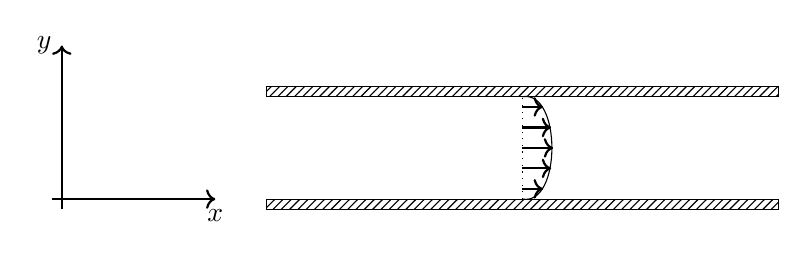
\begin{tikzpicture}[scale=1.3]
 \draw [pattern=north east lines] (0,0) -- (0,-0.1) -- (5,-0.1) -- (5,0) -- cycle;
 \draw [pattern=north east lines] (0,1) -- (0,1.1) -- (5,1.1) -- (5,1) -- cycle;

 \draw [->,thick] (-2,-0.1)--(-2,1.5) node[left] {$y$};
 \draw [->,thick] (-2.1,0)--(-0.5,0) node[below] {$x$};
 
 \draw [dotted] (2.5,0.0) to (2.5,1.0);
 \draw  (2.5,0.0) to [bend right=100] (2.5,1.0);
 
 \draw [->,thick] (2.5,0.9) to (2.7,0.9);
 \draw [->,thick] (2.5,0.7) to (2.78,0.7);
 \draw [->,thick] (2.5,0.5) to (2.8,0.5);
 \draw [->,thick] (2.5,0.3) to (2.78,0.3);
 \draw [->,thick] (2.5,0.1) to (2.7,0.1);
\end{tikzpicture}
\end{center}
\label{poiseuille}
\end{figure}

\noindent
The velocity profile equation is shown below:

\begin{equation}
 u = \frac{4 u_{max}}{L^2} y \big[ L - y \big]
\end{equation}

\medskip
\noindent
where $u_{max}$ is maximum velocity and its value is 
$u_{max} = 1.5$, $L$ is non-dimensional length 
between the plates and its value is 
$L = 1$
and $y$ is the vertical coordinates and it varies 
between $y = \big[ 0,1 \big]$.
The domain was discretized using a linear triangular mesh
with 3835 nodes and 7299 elements.
The \ref{velocidade poiseuille} shows the steady state velocity profile
when $Re=100$.
It is possible to observe that the numerical
solution converges to the analytical solution.

\vspace{1cm}
\begin{figure}[H]
     \caption{
Steady state velocity profile when $Re=100$ and the comparison between
the numerical and analytical solution for Poiseuille flow.} 
     \centering
     \includegraphics[scale=1]{./02_chaps/cap_validation/figure/poiseuille_velocity.pdf}\\
     \medskip
     \label{velocidade poiseuille}
\end{figure}

\newpage
The \ref{erro relativo poiseuille tabela} shows the relative error 
between the numerical solution and the analytical solution 
for several unstructured linear triangular meshes, ranging 
from 100 to 25600 linear triangular elements. For the mesh 
with 7299 elements as in the case of this benchmark problem, 
the estimated relative error for the velocity field is 0.4\%.

\vspace{0.5cm}
\begin{table}[H]
\centering
\begin{tabular}{ccc}
\toprule
\textbf{Elements} & \textbf{Error} (\%) \\
\midrule
100 & 25.00 \\
400 & 7.47 \\
1600 & 2.11 \\
6400 & 0.61 \\
25600 & 0.17 \\
\bottomrule
\end{tabular}
\caption{The relative error of numerical solution for several elements numbers in an unstructured linear triangular mesh.}
\label{erro relativo poiseuille tabela}
\end{table}

\noindent
\medskip
The relative error was estimated as:

\begin{equation}
 \mathit{Error} = \sqrt{\frac{\sum{(v_{n} - v_{a})^{2} }}{\sum |v_{a}|^{2} }}
\end{equation}

\noindent
where $v_{n}$ is the numerical velocity fielf and
$v_{a}$ is the analytical velocity field.

\bigskip
The \ref{ordem de convergencia poiseuille} presents the relative error 
of the numerical solution with the first and second order convergence 
curves on a log-log scale. As can be seen, the relative error of 
the numerical solution for Poiseuille flow has the form of 
first order convergence. Thus, when increasing the number of elements, 
the relative error of the numerical solution regresses linearly.
A possible cause is due to the vorticity boundary condition used 
in this work. Therefore, the use of the 2a-order boundary condition
would possibly improve the order convergence of the numerical
solution. However, it is necessary to be investigated. 


\begin{figure}[H]
     \caption{Convergence order in log-log scale:
It is estimated the the relative error of numerical solution has
first order convergence.}
     \centering
     \includegraphics[scale=1]{./02_chaps/cap_validation/figure/poiseuille_error.pdf}\\
     \medskip
     \label{ordem de convergencia poiseuille}
\end{figure}




\section{\textbf{Escoamento de Poiseuille em Meio Domínio}} 
\label{half poiseuille}

Nesta seção é apresentado a simulação do escoamento
de \textit{Poiseuille} na metade do domínio. Dessa forma,
a condição de contorno de superfície livre de escorregamento
é necessária no eixo de simetria.
A \ref{half poiseuille} apresenta esquematicamente este escoamento com o
eixo de simetria especificado e
o perfil do campo de velocidade esperado.

\begin{figure}[H]
\begin{center}
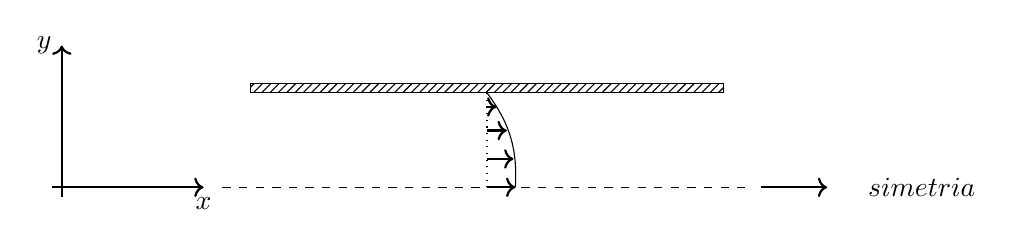
\begin{tikzpicture}[scale=1.2]
 \draw [pattern=north east lines] (0,1) -- (0,1.1) -- (5,1.1) -- (5,1) -- cycle;
 \draw [dashed] (-0.3,0.0) to (5.3,0.0);

 \draw [->,thick] (-2,-0.1)--(-2,1.5) node[left] {$y$};
 \draw [->,thick] (-2.1,0)--(-0.5,0) node[below] {$x$};

 \draw [->,thick] (5.4,0.0)--(6.1,0.0);
 \node [draw=none] at (7.1,0.0) {$simetria$};
 
 \draw [dotted] (2.5,0.0) to (2.5,1.0);
 \draw  (2.8,0.0) to [bend right=20] (2.5,1.0);
 
 \draw [->,thick] (2.5,0.0) to (2.8,0.0);
 \draw [->,thick] (2.5,0.3) to (2.78,0.3);
 \draw [->,thick] (2.5,0.6) to (2.71,0.6);
 \draw [->,thick] (2.5,0.85) to (2.6,0.85);
\end{tikzpicture}
\end{center}
\caption{Escoamento de Poiseuille em Meio Domínio}
\label{half poiseuille}
\end{figure}

\noindent
O perfil de velocidade que este escoamento adquire 
é dado pela equação abaixo:

\begin{equation}
 u = u_{max} \big[ 1 - \frac{y^{2}}{L^{2}} \big]
\end{equation}


\medskip
\noindent
onde $u_{max}$ é a velocidade máxima e seu valor é
$u_{max} = 1.5$, $L$ é a largura não dimensional
entre a placa e o eixo de simetria, seu valor é $L = 1$
e $y$ é a distância entre a placas e o eixo de simetria,
a mesma varia entre $y = \big[ 0,1 \big]$.
O domínio foi discretizado utilizando uma malha 
triangular linear com 3835 nós e 7299 elementos. 

\medskip
\noindent
As condições de contorno utilizadas foram:

\begin{itemize}
     \item \textit{condição de entrada}:
      a componente normal da velocidade $v=0$ enquanto a componente tangencial da velocidade é $u = 1$.                 
      A função de corrente também é especificada e seu valor é definido segundo a equação da continuidade  
      para um fluido incompressível. Dessa forma, seu valor será $\psi = y$.

     \item \textit{condição de não escorregamento}: esta condição é utilizada na placa superior, 
      onde todas as componentes da velocidade são especificadas    
      com os valores $u=0$ e $v=0$.                       
      A função de corrente também é espeficado com o valor $\psi=1$.               
      
     \item \textit{condição de saída}: O valor da função de corrente é especificado $\psi=y$. As derivadas das 
     componentes tangencial e normal da velocidade possuem o 
     valor nulo, isto é,
      $\partial u/\partial n = 0$ e
      $\partial v/\partial n = 0$ respectivamente.   

     \item \textit{condição de livre escorregamento}: esta condição é utilizada no eixo de simetria.
      A componente normal da velocidade e a função de corrente possuem seus valores especificados,
      tais como $v=0$ e $\psi=0$ respectivamente. A derivada da componente tangencial da velocidade
      possuei o valor nulo $\partial u/\partial n = 0$.
\end{itemize}

\medskip
A \ref{velocidade half poiseuille} apresenta a evolução 
do perfil de velocidade no tempo quando o $Re=100$, além do comparativo
entre a solução numérica e a solução analítica no estado permanente do
problema proposto. É possível observar um pequeno desvio entre a solução numérica
e a solução analítica próximo ao eixo de simetria. 

\begin{figure}[H]
     \centering
     \includegraphics[scale=1]{./02_chaps/cap_validation/figure/half_poiseuille_velocity.pdf}\\
     \medskip
     \caption{Evolução do perfil de velocidade no tempo para $Re=100$ e
     a comparação da solução numérica com a solução analítica para o Escoamento de Poiseuille em Meio Domínio.}
     \label{velocidade half poiseuille}
\end{figure}

\newpage


\section{\textbf{Escoamento em uma Cavidade com Tampa Móvel}} 
\label{cavity}

A flow in a cavity where the side and bottom walls are fixes and 
the cover moves at a constant velocity such as \textit{$U_{top}=1$} 
is known as \textit {Lid-driven Cavity flow}.
In addition to 
yhe streamfunction is set null value in all boundary, 
because there is no volumetric flux crossing the boundaries 
in lid-driven cavity flow.
The \ref{cavity} presents schematically this flow and 
the expected velocity field.

\vspace{1cm}
\begin{figure}[H]
\begin{center}
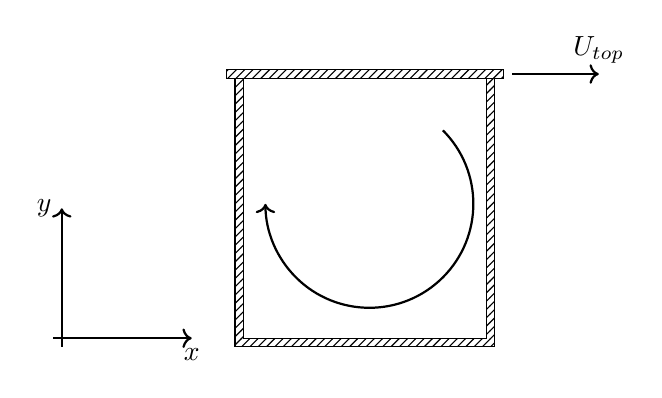
\begin{tikzpicture}[scale=1.1]
 \draw [pattern=north east lines] (0,-0.1) -- (3,-0.1) -- (3,3) -- (2.9,3) -- (2.9,0) -- (0.1,0) -- (0.1,3) -- (0,3) -- cycle;
 \draw [pattern=north east lines] (-0.1,3) -- (-0.1,3.1) -- (3.1,3.1) -- (3.1,3) -- cycle;

 \draw [->,thick] (3.2,3.05)--(4.2,3.05) node[above] {$U_{top}$};

 \draw [->,thick] (2.4,2.4) arc (45:-180:1.2);
 
 \draw [->,thick] (-2,-0.1)--(-2,1.5) node[left] {$y$};
 \draw [->,thick] (-2.1,0)--(-0.5,0) node[below] {$x$};

\end{tikzpicture}
\end{center}
\caption{Lid-driven Cavity Flow}
\label{cavity}
\end{figure}

\bigskip
The benchmark problem were simulated with the following 
Reynolds numbers (\textit{Re}): 10, 100, 400 and 1000.
The \ref{velocity vx cavity} and \ref{velocity vy cavity} 
prsent the profile of $u$ and $v$, respectively,
for steady state in several Reynolds number. 
They were compared with 
Ghia et al. (1982) \cite{ghia1982} and 
Marchi et al. (2009) \cite{marchi2009}. 
The domain was discretized using a linear triangular mesh 
with 1563 nodes and 2988 elements.

\begin{center}
\begin{figure}[H]
     \centering
     \begin{minipage}{.5\linewidth}
      \centering
      \includegraphics[scale=0.53]{./02_chaps/cap_validation/figure/Re_10_u_profile.pdf}\\
      (a)
     \end{minipage}%
     \begin{minipage}{.5\linewidth}
      \centering
      \includegraphics[scale=0.53]{./02_chaps/cap_validation/figure/Re_100_u_profile.pdf}\\
      (b)
     \end{minipage}
     \begin{minipage}{.5\linewidth}
      \centering
      \includegraphics[scale=0.53]{./02_chaps/cap_validation/figure/Re_400_u_profile.pdf}\\
      (c)
     \end{minipage}%
     \begin{minipage}{.5\linewidth}
      \centering
      \includegraphics[scale=0.53]{./02_chaps/cap_validation/figure/Re_1000_u_profile.pdf}\\
      (d)
     \end{minipage}
     \medskip
     \caption{The tangential velocity $u$ profile in central line of cavity ($x=0.5$) for several Reynolds number:
     (a) 10
     (b) 100
     (c) 400
     (d) 1000.}
     \label{velocity vx cavity}
\end{figure}
\end{center}

\begin{figure}[H]
     \centering
     \begin{minipage}{.5\linewidth}
      \centering
      \includegraphics[scale=0.53]{./02_chaps/cap_validation/figure/Re_10_v_profile.pdf}\\
      (a)
     \end{minipage}%
     \begin{minipage}{.5\linewidth}
      \centering
      \includegraphics[scale=0.53]{./02_chaps/cap_validation/figure/Re_100_v_profile.pdf}\\
      (b)
     \end{minipage}
     \begin{minipage}{.5\linewidth}
      \centering
      \includegraphics[scale=0.53]{./02_chaps/cap_validation/figure/Re_400_v_profile.pdf}\\
      (c)
     \end{minipage}%
     \begin{minipage}{.5\linewidth}
      \centering
      \includegraphics[scale=0.53]{./02_chaps/cap_validation/figure/Re_1000_v_profile.pdf}\\
      (d)
     \end{minipage}
     \medskip
     \caption{The normal velocity $v$ profile in central line of cavity ($y=0.5$) for several Reynolds number:
     (a) 10
     (b) 100
     (c) 400
     (d) 1000.}
     \label{velocity vy cavity}
\end{figure}



\section{\textbf{Escoamento Puramente Convectivo}} 
\label{convection}

The transport of a scalar according to a parabolic function and 
submitted to a monophase flow of a Newtonian and incompressible fluid 
with a high number of \textit{Reynolds} 
($\textit{Re} \rightarrow \infty$) is known as a 
\textit{Pure Advection flow}. In this type of flow, 
it is expected that the scalar will not diffuse. 
For approximation methods like \textit{FEM} and \textit{FDM}, 
it is possible to observe the presence of spurious oscillations. 
As mentioned earlier, several schemes can be used to reduce these 
numerical oscillations. In this section, we will present the use 
of the \textit{semi-Lagrangian} scheme to reduce spurious oscillations 
compared to the \textit{Taylor-Galerkin} Method. 
The \ref{conveccao} presents schematically the problem and 
the dynamics of scalar transport.

\vspace{0.5cm}
\begin{figure}[H]
\begin{center}
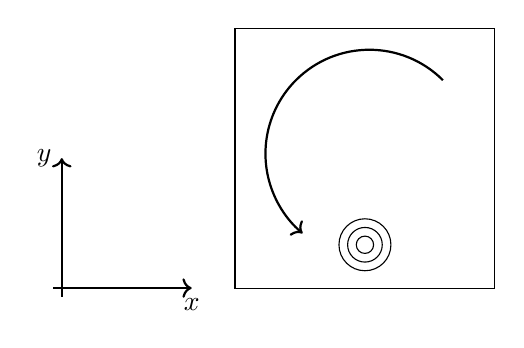
\begin{tikzpicture}[scale=1.1]
 \draw (0,0) -- (3,0) -- (3,3) -- (0,3) -- cycle;

 \draw [->,thick] (2.4,2.4) arc (45:230:1.2);
 
 \draw [->,thick] (-2,-0.1)--(-2,1.5) node[left] {$y$};
 \draw [->,thick] (-2.1,0)--(-0.5,0) node[below] {$x$};

 \draw (1.5,0.5) circle (0.3);
 \draw (1.5,0.5) circle (0.2);
 \draw (1.5,0.5) circle (0.1);

\end{tikzpicture}
\end{center}
\caption{Transport of a scalar in Pure Advection Flow.}
\label{conveccao}
\end{figure}

\medskip
\noindent
The scalar transport $\alpha$ for a pure advection flow is shown below:


\begin{equation}
 \frac{\partial \alpha}{\partial t} 
 + 
 \textbf{c} \cdot \nabla \alpha
 = 0
\end{equation}

\noindent
where is relative velocity and it is calculated by 
$\textbf{c} = \textbf{v} - \hat{\textbf{v}}$,
$\textbf{v}$ is material velocity field and its components are
defined as: $u = -y$ e $v = x$,
$\hat{\textbf{v}}$ is the mesh velocity and it is calculated
by the Eq. \ref{mesh velocity eq}. 
Therefore, it is expected that given an initial scalar field, 
it will be displaced by the velocity field without diffusion, 
that is, its profile should not be changed while the flow occurs. 
Any change in the scalar field profile is considered a numerical error.
The initial scalar field was defined by a parabolic
profile $c = 1 - x^2 - y^2$, where $x$ and $y$ are the spatial components.



\medskip
The \ref{perfil c} presents the comparison between the scalar field
profile $c$ for the semi-Lagrangian and Taylor-Galerkin methods in 
several positions on the axis of rotation as the flow occurs. 
It is possible to observe that in both methods the spurious oscillations 
are presented. In the Taylor-Galerkin method, however, 
such oscillations are dampened in contrast to the Galerkin method 
where we can observe that spurious oscillations increase and 
the scalar field profile becomes completely distorted.

\begin{center}
\begin{figure}[H]
     \centering
     \begin{minipage}{.5\linewidth}
      \centering
      \includegraphics[scale=0.53]{./02_chaps/cap_validation/figure/convection_0.pdf}\\
      (a)
     \end{minipage}%
     \begin{minipage}{.5\linewidth}
      \centering
      \includegraphics[scale=0.53]{./02_chaps/cap_validation/figure/convection_300.pdf}\\
      (b)
     \end{minipage}
     \begin{minipage}{.5\linewidth}
      \centering
      \includegraphics[scale=0.53]{./02_chaps/cap_validation/figure/convection_600.pdf}\\
      (c)
     \end{minipage}%
     \begin{minipage}{.5\linewidth}
      \centering
      \includegraphics[scale=0.53]{./02_chaps/cap_validation/figure/convection_950.pdf}\\
      (d)
     \end{minipage}
     \medskip
     \caption{Comparison of $c$ profile for the Galerkin e Taylor-Galerkinmethod in several positions on the axis of rotation: 
     (a) initial, 
     (b) 1/4 rotation,
     (c) 1/2 rotation and
     (d) 3/4 rotation.}
     \label{perfil c}
\end{figure}
\end{center}

\vspace{-1cm}
The \ref{galerkin} and \ref{taylor} show the spatial arrangement 
of spurious oscillations for the Galerkin and Taylor-Galerkin methods 
respectively. As mentioned earlier, the oscillations presented 
in the Galerkin method completely distort the scalar field $c$ 
while in the Taylor-Galerkin method, they are dampened as expected. 
Therefore, for problems where spurious oscillations are present, 
the Taylor-Galerkin method is superior to the Galerkin method.

\vspace{0.5cm}
\begin{figure}[H]
     \centering
     \begin{minipage}{.5\linewidth}
      \centering
      \includegraphics[scale=0.2]{./02_chaps/cap_validation/figure/galerkin_0.png}\\
      (a)
     \end{minipage}%
     \begin{minipage}{.5\linewidth}
      \centering
      \includegraphics[scale=0.2]{./02_chaps/cap_validation/figure/galerkin_300.png}\\
      (b)
     \end{minipage}
     \begin{minipage}{.5\linewidth}
      \centering
      \includegraphics[scale=0.2]{./02_chaps/cap_validation/figure/galerkin_600.png}\\
      (c)
     \end{minipage}%
     \begin{minipage}{.5\linewidth}
      \centering
      \includegraphics[scale=0.21]{./02_chaps/cap_validation/figure/galerkin_950.png}\\
      (d)
     \end{minipage}
     \medskip
     \caption{
Spurious oscillations for the Galerkin method in several positions of the axis of rotation:	
     (a) initial, 
     (b) 1/4 rotation,
     (c) 1/2 rotation and
     (d) 3/4 rotation.}
     \label{galerkin}
\end{figure}

\begin{figure}[H]
     \centering
     \begin{minipage}{.5\linewidth}
      \centering
      \includegraphics[scale=0.2]{./02_chaps/cap_validation/figure/taylor_0.png}\\
      (a)
     \end{minipage}%
     \begin{minipage}{.5\linewidth}
      \centering
      \includegraphics[scale=0.2]{./02_chaps/cap_validation/figure/taylor_300.png}\\
      (b)
     \end{minipage}
     \begin{minipage}{.5\linewidth}
      \centering
      \includegraphics[scale=0.2]{./02_chaps/cap_validation/figure/taylor_600.png}\\
      (c)
     \end{minipage}%
     \begin{minipage}{.5\linewidth}
      \centering
      \includegraphics[scale=0.2]{./02_chaps/cap_validation/figure/taylor_950.png}\\
      (d)
     \end{minipage}
     \medskip
     \caption{
Spurious oscillations for the Taylor-Galerkin method in several positions of the axis of rotation:	
     (a) initial, 
     (b) 1/4 rotation,
     (c) 1/2 rotation and
     (d) 3/4 rotation.}
     \label{taylor}
\end{figure}




\chapter{\textbf{RESULTS}}
\label{resultados}

\section{\textbf{Introduction}} 
In this chapter, the results of numerical simulations for 
blood flow in a coronary artery are presented. 
The lumen radius of the coronary artery used was $R=0.0015m$, 
the viscosity used was $\mu=0.0035Pa.s$ and the density used was
$\rho=1060kg/m^3$ as suggested by Bozsak, Chomaz and Barakat (2014)
 \cite{bozsak2014}. According to Kessler et al. (1998) 
\cite{kessler1998}, the blood velocity in the coronary artery 
is $u=12cm/s$. Thus, the Reynolds number used will be 
$Re=54.5$. 

\medskip
The Navier-Stokes equation is used according to the 
vorticity-streamfunction formulation with 
the species transport equation for two geometries proposed 
by Wang et al. (2017) \cite{wang2017}, however modified to 
cartesian coordinates as shown in \ref{coronary artery geo}. 
In the section \ref{canal curvado com stent}, the numerical 
simulation for the coronary artery with atherosclerosis 
and a drug-eluting stent in a curved channel model 
is presented for several 
\textit{Schmidt} number, such as $1$, $10$, $100$ and $1000$. 
In the \ref{canal real com stent}, the real coronary 
artery with atherosclerosis and a drug-eluting stent is also 
simulated with several numbers of \textit{Schmidt} number 
as in the previous section.
Due to symmetry, only half of the domain is shown. 
The simulation was visualized using the \textit{Paraview} open-source 
software proposed by Henderson (2007) \cite{paraview}.


\begin{figure}[H]
     \caption{Non-dimensional domain for the blood flow in coronary artery
     The radius used was $R=1$ and and the lumen length was $L=10R$.}
     \begin{center}
     \begin{minipage}{.45\linewidth}
     \begin{center}
      \includegraphics[scale=0.22]{./02_chaps/cap_solution/figure/CurvedStrut.png}\\
     (a) Curved Channel
     \end{center}
     \end{minipage}%
     \begin{minipage}{.45\linewidth}
     \begin{center}
      \includegraphics[scale=0.22]{./02_chaps/cap_solution/figure/RealStrut.png}\\
     (b) Real Channel
     \end{center}
     \end{minipage}\\[3mm]
     \end{center}
     \source Source: Wang et al. (2017) \cite{wang2017}
     \label{coronary artery geo}
\end{figure}


%\section{\textbf{Curved Channel}} 
%\label{canal curvado}
%For the case where the coronary artery has atherosclerosis, 
the problem is modeled as a flow between curved plates. 
The geometry used promotes a smooth reduction of the 
distance between the upper wall and symmetry axis of the channel. 
Due to atherosclerosis, 40\% channel obstruction was considered 
and the domain was discretized using 10261 nodes and 23049 
linear triangular elements. 

\par 
The \ref{velocity evolution curved} shows the unsteady velocity 
profile in the middle of the channel ($x=5R$). 
As we can see, the maximum non-dimensional value of the velocity field 
reaches $ u=2.3$ when the artery has atherosclerosis, that is, 
there is an increase of $53$\% of the maximum velocity when 
compared to the artery without atherosclerosis as shown in 
\ref{velocidade half poiseuille}.



\begin{figure}[H]
     \centering
     \includegraphics[scale=1]{./02_chaps/cap_solution/figure/vel_Curved_evol.pdf}\\
     \caption{The unsteady velocity profile for the curved channel.}
     \label{velocity evolution curved}
\end{figure}

\newpage
The \ref{velocity field curved} shows the evolution in time and space 
of the velocity field for half of the domain
The velocity field is represented with non-dimensional values 
where the red color refers to the value $u=2.3$ and 
the blue color $u=0$ approximately. Converting to dimensional values 
we have $u=27.6cm/s$ and $u=0cm/s$ respectively.

\vspace{2cm} 
\begin{figure}[H]
     \begin{minipage}{.50\linewidth}
      \centering
      \includegraphics[scale=0.175]{./02_chaps/cap_solution/figure/vel_Curved200.png}\\
      t = 0.1
     \end{minipage}%
     \begin{minipage}{.50\linewidth}
      \centering
      \includegraphics[scale=0.172]{./02_chaps/cap_solution/figure/vel_Curved1000.png}\\
      t = 0.5
     \end{minipage}
     \begin{minipage}{.50\linewidth}
     \medskip
      \centering
      \includegraphics[scale=0.175]{./02_chaps/cap_solution/figure/vel_Curved2000.png}\\
      t = 1.0
     \end{minipage}%
     \begin{minipage}{.50\linewidth}
     \medskip
      \centering
      \includegraphics[scale=0.175]{./02_chaps/cap_solution/figure/vel_Curved6000.png}\\
      t = 3.0
     \end{minipage}
     \begin{minipage}{.50\linewidth}
      \centering
      \includegraphics[scale=0.175]{./02_chaps/cap_solution/figure/vel_Curved8000.png}\\
      t = 4.0
     \end{minipage}%
     \begin{minipage}{.50\linewidth}
      \centering
      \includegraphics[scale=0.175]{./02_chaps/cap_solution/figure/vel_Curved10000.png}\\
      t = 5.0
     \end{minipage}
     \begin{minipage}{.50\linewidth}
     \medskip
      \centering
      \includegraphics[scale=0.175]{./02_chaps/cap_solution/figure/vel_Curved14000.png}\\
      t = 7.0
     \end{minipage}%
     \begin{minipage}{.50\linewidth}
     \medskip
      \centering
      \includegraphics[scale=0.175]{./02_chaps/cap_solution/figure/vel_Curved20000.png}\\
      t = 10.0
     \end{minipage}
     \medskip
     \caption{Time and space evolution of the velocity field for curved channel.}
     \label{velocity field curved}
\end{figure}

\newpage


\section{\textbf{Curved Channel with Drug-Eluting Stent}} 
\label{canal curvado com stent}
Para este caso, o stent farmacológico é colocado na parte superior 
do canal curvado. O mesmo é modelado por 10 semi círculos uniformemente
espaçados. Assim como no caso anterior, foi considerado uma obstrução
de 40\% do canal devido a aterosclerose e o domínio foi
discretizado com 15875 nós e 35408 elementos triangulares lineares. \par
A \ref{velocity evolution curved stent} apresenta o perfil
de velocidade transiente ao longo da coordenada $y$ no
meio do canal ($x=5R$). 
Como podemos observar, 
o valor adimensional máximo do campo de velocidade
chega a $u=3.6$ quando o stent é implantado, isto é,
possuímos um aumento de $56$\% quando comparado com
a artéria apenas com aterosclerose como no caso anterior (ver seção \ref{canal curvado}).

\begin{figure}[H]
     \centering
     \includegraphics[scale=1]{./02_chaps/cap_solution/figure/vel_CurvedStrut_evol.pdf}\\
     \caption{Evolução no tempo do perfil da velocidade para o Canal Curvado com Stent Farmacológico.}
     \label{velocity evolution curved stent}
\end{figure}

\newpage
A \ref{velocity field curved stent} apresenta a evolução no tempo e no espaço
do campo de velocidade para a metade do domínio já que os resultados são simétricos
na direção $y$. O campo de velocidade é representado com os valores adimensionais
onde a cor vermelha se refere ao valor $u=3.6$ e a cor azul $u=0$. 
Transformando em valores dimensionais temos $u=43.2 cm/s$ e $u=0 cm/s$ respectivamente. 

\vspace{2cm} 
\begin{figure}[H]
     \begin{minipage}{.50\linewidth}
      \centering
      \includegraphics[scale=0.12]{./02_chaps/cap_solution/figure/vel_CurvedStrut200.png}\\
      t = 0.1
     \end{minipage}%
     \begin{minipage}{.50\linewidth}
      \centering
      \includegraphics[scale=0.12]{./02_chaps/cap_solution/figure/vel_CurvedStrut1000.png}\\
      t = 0.5
     \end{minipage}
     \begin{minipage}{.50\linewidth}
     \medskip
      \centering
      \includegraphics[scale=0.12]{./02_chaps/cap_solution/figure/vel_CurvedStrut2000.png}\\
      t = 1.0
     \end{minipage}%
     \begin{minipage}{.50\linewidth}
     \medskip
      \centering
      \includegraphics[scale=0.12]{./02_chaps/cap_solution/figure/vel_CurvedStrut6000.png}\\
      t = 3.0
     \end{minipage}
     \begin{minipage}{.50\linewidth}
      \centering
      \includegraphics[scale=0.12]{./02_chaps/cap_solution/figure/vel_CurvedStrut8000.png}\\
      t = 4.0
     \end{minipage}%
     \begin{minipage}{.50\linewidth}
      \centering
      \includegraphics[scale=0.12]{./02_chaps/cap_solution/figure/vel_CurvedStrut10000.png}\\
      t = 5.0
     \end{minipage}
     \begin{minipage}{.50\linewidth}
     \medskip
      \centering
      \includegraphics[scale=0.12]{./02_chaps/cap_solution/figure/vel_CurvedStrut14000.png}\\
      t = 7.0
     \end{minipage}%
     \begin{minipage}{.50\linewidth}
     \medskip
      \centering
      \includegraphics[scale=0.12]{./02_chaps/cap_solution/figure/vel_CurvedStrut20000.png}\\
      t = 10.0
     \end{minipage}
     \medskip
     \caption{Evolução no tempo e no espaço do campo de velocidade para o Canal Curvado com Stent Farmacológico.}
     \label{velocity field curved stent}
\end{figure}


\vspace{1cm}
Conforme mencionado por Lucena et al. (2017) \cite{lucena2017}, é estimado que $47$\% do fármaco é difundido na corrente sanguínea.
A \ref{conc field curved stent sc 1} e a \ref{conc field curved stent sc 10} 
apresentam a evolução no tempo e no espaço
do campo da concentração para a metade do domínio devido a simetria para diversos números de \textit{Schmidt}
tais como: $1$ e $10$ respectivamente.
A concentração é representado com os valores adimensionais
onde a cor vermelha representa $100$\% e a cor azul representa $0$\% 
dessa concentração que é difundida na corrente sanguínea. 
É possível observar que o número de Schmidt influencia
diretamente no transporte do fármaco na corrente sanguínea. Para elevados valores do
número de \textit{Schmidt}, o transporte de espécie química torna-se puramente convectivo.

\begin{figure}[H]
     \begin{minipage}{.50\linewidth}
      \centering
      \includegraphics[scale=0.12]{./02_chaps/cap_solution/figure/conc1_CurvedStrut200.png}\\
      t = 0.1
     \end{minipage}%
     \begin{minipage}{.50\linewidth}
      \centering
      \includegraphics[scale=0.12]{./02_chaps/cap_solution/figure/conc1_CurvedStrut1000.png}\\
      t = 0.5
     \end{minipage}
     \begin{minipage}{.50\linewidth}
     \medskip
      \centering
      \includegraphics[scale=0.12]{./02_chaps/cap_solution/figure/conc1_CurvedStrut2000.png}\\
      t = 1.0
     \end{minipage}%
     \begin{minipage}{.50\linewidth}
     \medskip
      \centering
      \includegraphics[scale=0.12]{./02_chaps/cap_solution/figure/conc1_CurvedStrut6000.png}\\
      t = 3.0
     \end{minipage}
     \begin{minipage}{.50\linewidth}
      \centering
      \includegraphics[scale=0.12]{./02_chaps/cap_solution/figure/conc1_CurvedStrut8000.png}\\
      t = 4.0
     \end{minipage}%
     \begin{minipage}{.50\linewidth}
      \centering
      \includegraphics[scale=0.12]{./02_chaps/cap_solution/figure/conc1_CurvedStrut10000.png}\\
      t = 5.0
     \end{minipage}
     \begin{minipage}{.50\linewidth}
     \medskip
      \centering
      \includegraphics[scale=0.12]{./02_chaps/cap_solution/figure/conc1_CurvedStrut14000.png}\\
      t = 7.0
     \end{minipage}%
     \begin{minipage}{.50\linewidth}
     \medskip
      \centering
      \includegraphics[scale=0.12]{./02_chaps/cap_solution/figure/conc1_CurvedStrut20000.png}\\
      t = 10.0
     \end{minipage}
     \medskip
     \caption{Evolução no tempo e no espaço do campo de espécie química para o Canal Curvado com Stent Farmacológico com $Sc=1$.}
     \label{conc field curved stent sc 1}
\end{figure}

\bigskip
\begin{figure}[H]
     \begin{minipage}{.50\linewidth}
      \centering
      \includegraphics[scale=0.12]{./02_chaps/cap_solution/figure/conc10_CurvedStrut500.png}\\
      t = 0.1
     \end{minipage}%
     \begin{minipage}{.50\linewidth}
      \centering
      \includegraphics[scale=0.12]{./02_chaps/cap_solution/figure/conc10_CurvedStrut2500.png}\\
      t = 0.5
     \end{minipage}
     \begin{minipage}{.50\linewidth}
     \medskip
      \centering
      \includegraphics[scale=0.12]{./02_chaps/cap_solution/figure/conc10_CurvedStrut5000.png}\\
      t = 1.0
     \end{minipage}%
     \begin{minipage}{.50\linewidth}
     \medskip
      \centering
      \includegraphics[scale=0.12]{./02_chaps/cap_solution/figure/conc10_CurvedStrut15000.png}\\
      t = 3.0
     \end{minipage}
     \begin{minipage}{.50\linewidth}
      \centering
      \includegraphics[scale=0.12]{./02_chaps/cap_solution/figure/conc10_CurvedStrut20000.png}\\
      t = 4.0
     \end{minipage}%
     \begin{minipage}{.50\linewidth}
      \centering
      \includegraphics[scale=0.12]{./02_chaps/cap_solution/figure/conc10_CurvedStrut25000.png}\\
      t = 5.0
     \end{minipage}
     \begin{minipage}{.50\linewidth}
     \medskip
      \centering
      \includegraphics[scale=0.12]{./02_chaps/cap_solution/figure/conc10_CurvedStrut35000.png}\\
      t = 7.0
     \end{minipage}%
     \begin{minipage}{.50\linewidth}
     \medskip
      \centering
      \includegraphics[scale=0.12]{./02_chaps/cap_solution/figure/conc10_CurvedStrut50000.png}\\
      t = 10.0
     \end{minipage}
     \medskip
     \caption{Evolução no tempo e no espaço do campo de espécie química para o Canal Curvado com Stent Farmacológico com $Sc=10$.}
     \label{conc field curved stent sc 10}
\end{figure}

\medskip


%\section{\textbf{Real Channel}} 
%\label{canal real}
%For this case, the numerical simulation is performed for a real 
coronary artery with atherosclerosis whose geometry was obtained 
through an image processing as suggested by Wang et al. (2017) 
\cite{wang2017}. This geometry is particular to each patient 
due to the patient health conditions. As in the previous cases, 
an channel obstruction of 40\% was considered due to atherosclerosis 
and the domain was discretized using 7632 nodes and 14665 linear 
triangular elements. 

\par 
The \ref{velocity evolution real} shows the velocity profile 
in the middle of the channel ($x=5R$). The maximum non-dimensional
 value of the velocity field reaches $u=2.25$. Thus, the 
curved geometry represents a good approximation as seen in 
\ref{velocity evolution curved}, 
such that the difference of maximum non-dimensional velocity value 
is about 2\%.
.

\begin{figure}[H]
     \centering
     \includegraphics[scale=1]{./02_chaps/cap_solution/figure/vel_Real_evol.pdf}\\
     \caption{The unsteady velocity profile for the real channel.}
     \label{velocity evolution real}
\end{figure}

\newpage
The 
\ref{velocity field real} 
shows the evolution in time and space of the velocity field for half of the
domain The velocity field is represented with non-dimensional values where the red color
refers to the value 
$u=2.25$
and the blue color 
$u=0$
approximately. 
Converting to dimensional
values we have 
$u = 27.0cm/s$
 and 
$u = 0cm/s$ 
respectively.

\vspace{2cm} 
\begin{figure}[H]
     \begin{minipage}{.50\linewidth}
      \centering
      \includegraphics[scale=0.12]{./02_chaps/cap_solution/figure/vel_Real200.png}\\
      t = 0.1
     \end{minipage}%
     \begin{minipage}{.50\linewidth}
      \centering
      \includegraphics[scale=0.12]{./02_chaps/cap_solution/figure/vel_Real1000.png}\\
      t = 0.5
     \end{minipage}
     \begin{minipage}{.50\linewidth}
     \medskip
      \centering
      \includegraphics[scale=0.12]{./02_chaps/cap_solution/figure/vel_Real2000.png}\\
      t = 1.0
     \end{minipage}%
     \begin{minipage}{.50\linewidth}
     \medskip
      \centering
      \includegraphics[scale=0.12]{./02_chaps/cap_solution/figure/vel_Real6000.png}\\
      t = 3.0
     \end{minipage}
     \begin{minipage}{.50\linewidth}
      \centering
      \includegraphics[scale=0.12]{./02_chaps/cap_solution/figure/vel_Real8000.png}\\
      t = 4.0
     \end{minipage}%
     \begin{minipage}{.50\linewidth}
      \centering
      \includegraphics[scale=0.12]{./02_chaps/cap_solution/figure/vel_Real10000.png}\\
      t = 5.0
     \end{minipage}
     \begin{minipage}{.50\linewidth}
     \medskip
      \centering
      \includegraphics[scale=0.12]{./02_chaps/cap_solution/figure/vel_Real14000.png}\\
      t = 7.0
     \end{minipage}%
     \begin{minipage}{.50\linewidth}
     \medskip
      \centering
      \includegraphics[scale=0.12]{./02_chaps/cap_solution/figure/vel_Real20000.png}\\
      t = 10.0
     \end{minipage}
     \medskip
     \caption{Time and space evolution of the velocity field for real channel.} 
     \label{velocity field real}
\end{figure}

\newpage


\section{\textbf{Real Channel with Drug-Eluting Stent}} 
\label{canal real com stent}
For this case, the numerical simulation is performed for a real 
coronary artery with atherosclerosis whose geometry was obtained 
through an image processing as suggested by Wang et al. (2017) 
\cite{wang2017}. This geometry is particular to each patient 
due to the patient health conditions. As in the previous cases, 
an channel obstruction of 40\% was considered due to atherosclerosis 
and the stent strut was modeled by
10 uniformly spaced semi-circles.
The domain was discretized using 11807 nodes and 26426 linear 
triangular elements. 

\medskip
The \ref{velocity evolution real stent} shows the unsteady velocity 
profile in the middle of the channel ($x=5R$). 
As we can see, the maximum non-dimensional value of the velocity field 
reaches $u=2.65$ when the stent is placed. 
However, this velocity may vary according to the 
coronary artery geometry for each patient.

\begin{figure}[H]
     \centering
     \includegraphics[scale=1]{./02_chaps/cap_solution/figure/vel_RealStrut_evol.pdf}\\
     \caption{
The unsteady velocity profile for real channel with drug-eluting stent.}
     \label{velocity evolution real stent}
\end{figure}

\newpage
The \ref{velocity field real stent} presents the evolution in 
time and space of the velocity field for half of the domain. 
The velocity field is represented with non-dimensional values 
where the red color refers to the $u=2.65$ value and the blue color 
$u=0$ value. Conveting to dimensional values, 
we have $u=31.8cm/s$ and $u=0cm/s$ respectively.

\vspace{2cm}
\begin{figure}[H]
     \begin{minipage}{.50\linewidth}
      \centering
      \includegraphics[scale=0.12]{./02_chaps/cap_solution/figure/vel_RealStrut200.png}\\
      t = 0.1
     \end{minipage}%
     \begin{minipage}{.50\linewidth}
      \centering
      \includegraphics[scale=0.12]{./02_chaps/cap_solution/figure/vel_RealStrut1000.png}\\
      t = 0.5
     \end{minipage}
     \begin{minipage}{.50\linewidth}
     \medskip
      \centering
      \includegraphics[scale=0.12]{./02_chaps/cap_solution/figure/vel_RealStrut2000.png}\\
      t = 1.0
     \end{minipage}%
     \begin{minipage}{.50\linewidth}
     \medskip
      \centering
      \includegraphics[scale=0.12]{./02_chaps/cap_solution/figure/vel_RealStrut6000.png}\\
      t = 3.0
     \end{minipage}
     \begin{minipage}{.50\linewidth}
      \centering
      \includegraphics[scale=0.12]{./02_chaps/cap_solution/figure/vel_RealStrut8000.png}\\
      t = 4.0
     \end{minipage}%
     \begin{minipage}{.50\linewidth}
      \centering
      \includegraphics[scale=0.12]{./02_chaps/cap_solution/figure/vel_RealStrut10000.png}\\
      t = 5.0
     \end{minipage}
     \begin{minipage}{.50\linewidth}
     \medskip
      \centering
      \includegraphics[scale=0.12]{./02_chaps/cap_solution/figure/vel_RealStrut14000.png}\\
      t = 7.0
     \end{minipage}%
     \begin{minipage}{.50\linewidth}
     \medskip
      \centering
      \includegraphics[scale=0.12]{./02_chaps/cap_solution/figure/vel_RealStrut20000.png}\\
      t = 10.0
     \end{minipage}
     \medskip
     \caption{
Time and space evolution of the velocity field for real channel with
drug-eluting stent.}
     \label{velocity field real stent}
\end{figure}

\vspace{1cm}
The \ref{conc field real stent sc 1} and 
\ref{conc field real stent sc 10} show the time and space evolution 
of the concentration field for several \textit{Schmidt} number, 
such as: $1$ and $10$ respectively. The concentration field is 
represented with the non-dimensional values where the red color 
represents $100$\% and the blue color represents $0$\% 
of the diffused concentration in the bloodstream. 
It is possible to observe that the \textit{Schmidt} number directly 
influences the drug transport in the blood flow. 
For high values of the \textit{Schmidt} number, 
the transport of chemical species becomes purely convective.

\begin{figure}[H]
     \begin{minipage}{.50\linewidth}
      \centering
      \includegraphics[scale=0.12]{./02_chaps/cap_solution/figure/conc1_RealStrut200.png}\\
      t = 0.1
     \end{minipage}%
     \begin{minipage}{.50\linewidth}
      \centering
      \includegraphics[scale=0.12]{./02_chaps/cap_solution/figure/conc1_RealStrut1000.png}\\
      t = 0.5
     \end{minipage}
     \begin{minipage}{.50\linewidth}
     \medskip
      \centering
      \includegraphics[scale=0.12]{./02_chaps/cap_solution/figure/conc1_RealStrut2000.png}\\
      t = 1.0
     \end{minipage}%
     \begin{minipage}{.50\linewidth}
     \medskip
      \centering
      \includegraphics[scale=0.12]{./02_chaps/cap_solution/figure/conc1_RealStrut6000.png}\\
      t = 3.0
     \end{minipage}
     \begin{minipage}{.50\linewidth}
      \centering
      \includegraphics[scale=0.12]{./02_chaps/cap_solution/figure/conc1_RealStrut8000.png}\\
      t = 4.0
     \end{minipage}%
     \begin{minipage}{.50\linewidth}
      \centering
      \includegraphics[scale=0.12]{./02_chaps/cap_solution/figure/conc1_RealStrut10000.png}\\
      t = 5.0
     \end{minipage}
     \begin{minipage}{.50\linewidth}
     \medskip
      \centering
      \includegraphics[scale=0.12]{./02_chaps/cap_solution/figure/conc1_RealStrut14000.png}\\
      t = 7.0
     \end{minipage}%
     \begin{minipage}{.50\linewidth}
     \medskip
      \centering
      \includegraphics[scale=0.12]{./02_chaps/cap_solution/figure/conc1_RealStrut20000.png}\\
      t = 10.0
     \end{minipage}
     \medskip
     \caption{
Time and space evolution of the concentration field for real channel 
with drug-eluting stent when the $Sc=1$.}
     \label{conc field real stent sc 1}
\end{figure}

\bigskip
\begin{figure}[H]
     \begin{minipage}{.50\linewidth}
      \centering
      \includegraphics[scale=0.115]{./02_chaps/cap_solution/figure/conc10_RealStrut500.png}\\
      t = 0.1
     \end{minipage}%
     \begin{minipage}{.50\linewidth}
      \centering
      \includegraphics[scale=0.115]{./02_chaps/cap_solution/figure/conc10_RealStrut2500.png}\\
      t = 0.5
     \end{minipage}
     \begin{minipage}{.50\linewidth}
     \medskip
      \centering
      \includegraphics[scale=0.115]{./02_chaps/cap_solution/figure/conc10_RealStrut5000.png}\\
      t = 1.0
     \end{minipage}%
     \begin{minipage}{.50\linewidth}
     \medskip
      \centering
      \includegraphics[scale=0.115]{./02_chaps/cap_solution/figure/conc10_RealStrut15000.png}\\
      t = 3.0
     \end{minipage}
     \begin{minipage}{.50\linewidth}
      \centering
      \includegraphics[scale=0.115]{./02_chaps/cap_solution/figure/conc10_RealStrut20000.png}\\
      t = 4.0
     \end{minipage}%
     \begin{minipage}{.50\linewidth}
      \centering
      \includegraphics[scale=0.115]{./02_chaps/cap_solution/figure/conc10_RealStrut25000.png}\\
      t = 5.0
     \end{minipage}
     \begin{minipage}{.50\linewidth}
     \medskip
      \centering
      \includegraphics[scale=0.115]{./02_chaps/cap_solution/figure/conc10_RealStrut35000.png}\\
      t = 7.0
     \end{minipage}%
     \begin{minipage}{.50\linewidth}
     \medskip
      \centering
      \includegraphics[scale=0.115]{./02_chaps/cap_solution/figure/conc10_RealStrut50000.png}\\
      t = 10.0
     \end{minipage}
     \medskip
     \caption{
ime and space evolution of the concentration field for real channel 
with drug-eluting stent when the $Sc=10$.}
     \label{conc field real stent sc 10}
\end{figure}


\newpage






%% ----- CONCLUSION  (03)
\pagebreak
\addcontentsline{toc}{chapter}{\hspace{1.7cm}\bfseries CONCLUSION}
\clearpage
\noindent\textbf{CONCLUSÃO}
$\!$\\

Neste trabalho foi apresentado a equação de Navier-Stokes
utilizando a formulação corrente-vorticidade
com a equação de transporte de espécie química em uma abordagem
do Método dos Elementos Finitos em que o esquema Taylor-Galerkin
foi aplicado às equações de governo. Como a formulação corrente-vorticidade
não apresenta o acoplamento entre a velocidade e pressão,
podemos utilizar o elemento triangular linear sem restrição
possibilitando assim uma facilidade na implementação do código
númerico além das variáveis envolvidas serem escalares e não vetoriais
como no caso das variáveis primitivas.

\medskip
Foi construído um código completo em linguagem de programação de alto nível 
usando o paradigma de orientação de objetos e a partir do presente momento,
possuímos uma plataforma de estudos de problemas de escoamento de fármacos
em artérias. O simulador é capaz também de descrever em detalhes problemas
envolvendo escoamento de fluidos newtonianos com transporte de natureza
escalar (como na concentração e na temperatura) devido a construção 
generalizada do código.

\medskip
O código numérico apresentou
resultados satisfatórios comparados às soluções analíticas dos
\textit{Escoamento de Couette}, \textit{Escoamento de Poiseuille}
e \textit{Escoamento de Poiseuille em Meio Domínio} onde a condição
de superfície livre escorregamento no eixo de simetria foi aplicada.
Foi simulado, também, o escoamento em uma cavidade com tampa móvel (\textit{lid-driven cavity flow})
onde os resultados foram comparados com aqueles apresentados por Ghia et al. (1982) \cite{ghia1982} e Marchi et al. (2009) \cite{marchi2009}
para vários números de Reynolds.
Por fim, foi apresentado a comparação
entre os esquemas \textit{Galerkin} e \textit{Taylor-Galerkin} para um
escoamento puramente convectivo de uma função parabólica onde foi
possível observar a eficácia do esquema \textit{Taylor-Galerkin}
em comparação ao esquema \textit{Galerkin} para a redução das
oscilações espúrias. 
Dessa forma, a validação do código numérico foi realizada
para problemas convectivos-difusivos bidimensionais em coordenadas cartesianas e submetido à condição de contorno de
\textit{Dirichlet}.

\medskip
O objetivo desse trabalho era conhecer a dinâmica do escoamento
sanguíneo em uma artéria coronária com aterosclerose e com 
stent farmacológico implantado. Dessa forma, foi apresentado a simulação
para quatro geometrias modeladas como bidimensionais e
em coordenadas cartesianas. 
Foi apresentado o perfil do campo de velocidade para as quatro geometrias propostas onde foi
possível observar o aumento da velocidade máxima quando o stent
farmacológico estava implantado.  
A simulação foi feita utilizando diversos números de \textit{Schmidt},
tais como $Sc = 1$ e $10$. Foi possível verificar na simulação que o número de
\textit{Schmidt} influencia diretamente no transporte do fármaco
na corrente sanguínea. Para elevados valores do número de \textit{Schmidt},
o transporte de espécie química torna-se puramente convectivo
e sua influência na parede da artéria deve ser verificada.

\vspace{0.7cm}
\noindent
Para trabalhos futuros, destacamos quatro desenvolvimentos:

\begin{itemize}
 \vspace{-0.3cm}
 \item Utilização do esquema \textit{Semi-Lagrangeano} para as derivadas materiais
       em substituição do esquema \textit{Taylor-Galerkin}
       para a redução das oscilações espúrias  

 \item Utilização das variáveis primitivas na equação de Navier-Stokes em uma abordagem 3D
 
 \item Modelar o escoamento sanguíneo como um problema multifásico

 \item Simular a transferência de espécie química na parede da artéria acoplado ao escoamento no lúmen.
\end{itemize}










%% ----- APPENDICES  (04) - optional
%\pagebreak
%\addcontentsline{toc}{chapter}{\hspace{1.7cm}\bfseries APPENDIX A - VITA}
%\noindent{\textbf{APÊNDICE A - PUBLICAÇÃO}
\bigskip

\lipsum[1]



%% ----- REFERENCES  
\pagebreak
\addcontentsline{toc}{chapter}{\hspace{1.7cm}\bfseries BIBLIOGRAPHY}
\def\bibname{BIBLIOGRAPHY} 

%% ----- BIBTEX DATABASE
\bibliographystyle{abnt-num}
\bibliography{references}	 % bibtex entries or 
%\bibliography{../../bib}	 % full path to bib database

%% ----- APPENDICES  (04) - optional
\pagebreak
\addcontentsline{toc}{chapter}{\hspace{1.7cm}\bfseries APÊNDICE - PUBLICAÇÕES}
\noindent{\textbf{APÊNDICE - PUBLICAÇÕES}
\bigskip

Durante a execução deste estudo, alguns trabalhos foram publicados
ou aceitos na forma de artigos em congressos. Este apêndice traz três desses trabalhos. 
Inicialmente é apresentado o trabalho aceito para publicação pelo 
\textit{17th Brazilian Congress of Thermal Sciences and Engineering (ENCIT)} que acontecerá
em Novembro de 2018.
Em seguida, apresentamos o trabalho publicado pelo 
\textit{X Congresso Nacional de Engenharia Mecânica (CONEM)} com identificação
doi://10.26678/ABCM.CONEM2018.CON18-1227 que ocorreu em Maio de 2018. 
Por fim, é apresentado
o trabalho publicado pelo 
\textit{II Congresso Brasileiro de Fluidodinâmica Computacional (CBCFD)} que
ocorreu em Junho de 2018.
Abaixo segue um pequeno resumo desses trabalhos:

\vspace{1cm}
\noindent
\textbf{BLOOD FLOW DYMANICS SIMULATION IN CORONARY ARTERY WITH DRUG-ELUTING STENT USING FINITE ELEMENT METHOD}\\
\textit{17th Brazilian Congress of Thermal Sciences and Engineering (ENCIT 2018)}\\
\textit{Novembro/2018} - Aceito para a publicação

\medskip
\noindent
The present work aims at developing a computational framework to simulate coronary artery flows in cartesian
coordinates. The Finite Element Method (FEM) is used to solve the governing equations of the blood flow in coronary
artery with drug-eluting stent placed. The blood was modeled as single-phase, incompressible and newtonian fluid. The
Navier-Stokes equation is shown according to the stream-vorticity formulation with coupled species transport equation.
The Taylor-Galerkin scheme were used to decrease spurious oscillations as seen for moderate to high Reynolds number.
The code proved to be effective by results
presented in validation cases. The dynamics of blood flow was shown to a coronary artery with atherosclerosis and
drug-eluting stent placed. Therefore, the streamfunction and vorticity formulation showed an useful approximation for to
calculate the velocity and concentration fields since the variables are scalars allowing then a smooth implemention.

\newpage
\noindent
\textbf{A NUMERICAL SIMULATION OF BLOOD FLOW DYNAMICS IN CORONARY ARTERY USING STREAMFUNCTION-VORTICITY FORMULATION}\\
\textit{X Congresso Nacional de Engenharia Mecânica (CONEM 2018)}\\
\textit{Maio/2018 - Publicado}\\
\textit{doi://10.26678/ABCM.CONEM2018.CON18-1227}

\medskip
\noindent
The present work aims at developing a computational framework to simulate coronary artery flows in cartesian
coordinates. An accurate method capable of capturing the flow dynamics is strictly required. In this paper a Finite
Element Method (FEM) is used to solve the governing equations of the motion of the blood flow found in coronary artery
as incompressible fluid using the stream-vorticity formulation with coupled mass transport.
The validation of the numerical solution was done by well-known benchmark lid-driven cavity problem and the results were
compared with others authors as well as the Hagen-Poiseuille flow for the case straight channel that was compared with
analytical solution. The streamfunction and vorticity formulation showed an useful approximation for to calculate the
velocity and concentration fields since the variables are scalars allowing then a smooth implemention.

\bigskip
\noindent
\textbf{BLOOD FLOW SIMULATION USING STREAM FUNCTION-VORTICITY FEM FORMULATION}\\
\textit{II Congresso Brasileiro de Fluidodinâmica Computacional (CBCFD 2018)}\\
\textit{Junho/2018 - Publicado}

\medskip
\noindent
The present work aims at developing a computational framework to simulate coronary artery
flows in cartesian coordinates. An accurate method capable of capturing the flow dynamics is
strictly required. In this paper a Finite Element Method (FEM) is used to solve the governing
equations of the motion of the blood flow found in coronary artery as incompressible fluid using
the stream-vorticity formulation with coupled species transport equation.
The results were shown for two-dimensional domain in complex geometries
of modeled coronary artery channel. The numerical simulation was performed using the stre-
amfunction and vorticity formulation with coupled species transport equation by finite element
method approach. The streamfunction and vorticity formulation showed a smotth implemen-
tion for to calulate the variables since they are scalars. However, there is a significant difference
between the results shown in cartesian coordinates and those shown by Wang et al. (2017) in
axisymmetric coordinates.



\includepdf[scale=0.95,pages=-]{./04_app/ENCIT2018_final.pdf}
\includepdf[scale=0.95,pages=-]{./04_app/CONEM2018.pdf}
\includepdf[scale=0.95,pages=-]{./04_app/CBCFD.pdf}

\null\newpage


\end{document}
%% -----END OF DOCUMENT

